

% Modelo da Dissertação de Mestrado da Escola Naval
% TMDEI Thesis EN Style
% 
% Baseado em MastersDoctoralThesis Version 1.2 by Vel (vel@latextemplates.com) and
% Johannes Böttcher, downloaded from (21/11/15):
% http://www.LaTeXTemplates.com
%
% Autores:
%  Vel (vel@ latextemplates. com)
%  Johannes Böttcher%
%
%  Adaptado para Thesis EN Style (JUL/2019) por 
%  Hilário Araújo (rocha.araujo@marinha.pt) 
%  Ricardo Moura (ricardo.pinto.moura@marinha.pt)
%
%%%%%%%%%%%%%%%%%%%%%%%%%%%%%%%%%%%%%%%%%

%-----------------------------------------%
%    CONFIGURAÇÃO INICIAl
%-----------------------------------------%

\documentclass[12pt, % O tamanho da fonte do documento padrão, opções: 10pt, 11pt (ter-se-ia que mudar tipo de letra para Arial) , 12pt (relembra-se que 12pt é o que está estipulado nas normas)
%oneside, % Dois lados (margens alternadas) para ligação por padrão, descomentar  para mudar para um lado (para desenho / leitura)
portuguese, %portuguese,% para Português; english para Inglês; Se mudar a língua convém apagar ficheiros temporários (e.g. 'make clean; make')
onehalfspacing, % espaçamento e meio, alternativas: singlespacing - Espaçamento de linha única; doublespacing (para fins de redação / leitura)
%draft, % Descomentar para ativar o modo de rascunho (sem imagens, sem links, caixas de texto overfull indicadas)
%nolistspacing, % Se o documento for de meio-espaço ou de espaçamento duplo, descomentar para definir o espaçamento nas listas como único
%liststotoc, % Descomentar para adicionar a lista de figuras / tabelas / etc ao índice (não recomendado)
%toctotoc, % Descomentear para adicionar o índice principal ao índice (não recomendado)
parskip, % Adicione espaço entre parágrafos (recomendado)
%nohyperref, % Descomentar para não carregar o pacote hyperref (não recomendado)
nohyperreflinkcolor, % links de hyperref (ligação à referência) não são coloridos (comentar para links de cores, por exemplo, para produzir uma versão somente eletrónica)
headsepline, % Descomentar para obter uma linha sob o cabeçalho
]{enStyle} % O arquivo de classe que especifica a estrutura do documento

\usepackage{tikz} % Em caso de necessidade para criar gráficos automaticamente na página (pode remover se tiver apenas gráficos por imagem)
%\usetikzlibrary{arrows} % Necessário se quiser inserir setas do pacote TiKZ (pode remover se não usar)

\usepackage{pgfplots} % Necessário se quiser desenhar plots de alta qualidade (pode remover se não usar)
\pgfplotsset{compat=newest}

\usepackage[framed,numbered,autolinebreaks,useliterate]{mcode}

%
% Next you have examples of admissable citation styles; we recomend using the authoryear-comp citation style (which resembles Harvard); don't forget to only uncomment one

% authoryear-comp: recommended citation style (e.g. (Buendía, 1860), (Buendía 1910, Arcadio 1940))
\usepackage[style=authoryear-comp,backend=biber,doi=true, %display DOI with link
     eprint=false, %display arxiv id etc
     maxnames=25, %number of names in List of references
     maxcitenames=3, % number of names for textcite command
     ]{biblatex} % Bibtex backend with the authoryear-comp citation style (authoryear citations, bibliography ordered alphabetically)

%\usepackage[backend=biber,
%     style=authoryear-comp, %style to use, other styles are nature, science or apa
%     sorting=none,
%     natbib=true,
%     url=false, 
%     doi=true, %display DOI with link
%     eprint=false, %display arxiv id etc
%     maxnames=25, %number of names in List of references
%     maxcitenames=2, % number of names for textcite command
%     autocite=superscript
%]{biblatex}

% numeric citation style (e.g. [1], [1-3])
%\usepackage[style=numeric-comp,sorting=none,backend=biber]{biblatex} % Bibtex backend with the numeric-comp citation style (numeric citations, bibliography ordered by appearance)

% alphabetic citation style (e.g. [Buendía10], [Buendía10, Arcadio40])
%\usepackage[style=alphabetic,sorting=none,backend=biber]{biblatex} % Bibtex backend with the alphabetic citation style (alphabetic citations, bibliography ordered by appearance)
\usepackage{esint}

\usepackage{mcode}




\addbibresource{mainbibliography.bib} % O nome da base de dados da sua bibliografia

\makeglossaries % cria o glossário


%----------------------------------------------------------------------------------------
%	INFORMAÇÃO SOBRE A TESE
%----------------------------------------------------------------------------------------

\thesistitle{Deteção de Alvos em Sistemas de Radares Passivos} % Escreva o título da tese, pode referenciar o titulo ao longa da dissertação utilizando o comando (\ttitle)

%\thesissubtitle{} % %Escreva o subtítulo da tese, pode referenciar o titulo ao longa da dissertação utilizando o comando (\subttitle)

\author{Afonso Lobo Sénica} % % Escreva o seu nome completo, pode referenciar o autor ao longa da dissertação utilizando o comando (\authorname)

\authorshort{Afonso Sénica} % % Escreva o seu 1º e último nome, pode referenciar o autor ao longa da dissertação utilizando o comando (\authorname)

\subjectarea{Engenharia Naval Ramo de Armas e Eletrónica} % Identifica a tua especialidade: Engenharia Naval Ramo de Armas e Eletrónica, Engenharia Naval Ramo de Mecânica, Marinha, Fuzileiros, Marinha e Administração Naval
%poderá referenciar-lo ao longo do seu trabalho com o comando (\areaname)

\supervisor{Paulo Alexandre Carapinha Marques} % O nome do seu supervisor, isto é usado na página da contra capa,  poderá referenciar-lo ao longo do seu trabalho com o comando (\supname)
\supervisorshort{Paulo Marques}

\cosupervisor{João Luís Reis Fidalgo Neves} % O nome do seu co-orientador, isto é usado na página da contra capa,  poderá referenciar-lo ao longo do seu trabalho com o comando (\cosupname) (comenta, se não tiveres co-orientador)
\cosupervisorshort{João Neves}

\keywords{Radar Passivo, Deteção, Processamento de Sinal, DVB-T (Digital Video Broadcasting - Terrestrial)} % Defina até 6 palavras-chave que descrevam melhor o seu trabalho, e poderá referenciar-las ao longo do seu trabalho com o comando (\keywordnames)

\conkeywords{Passive Radar, Detection, Signal Processing, DVB-T (Digital Video Broadcasting - Terrestrial)} %  Traduza as palavras do resumo e coloque-as aqui(\conkeywordnames)

\university{\href{https://escolanaval.marinha.pt}{Escola Naval}} % Nome da universidade e endereço web, , e poderá referenciar-la ao longo do seu trabalho com o comando \univname

\department{\href{http://department.university.com}{Departamento Ciência e Tecnologias}} % Nome do departamento e endereço web, e poderá referenciar-la ao longo do seu trabalho com o comando \deptname
% Classes e respetivos departamentos:
% EN-AEL E EN-MEC - Departamento Ciência e Tecnologias
% AN - Departamento de Humanidades e Gestão
% M - Departamento de Ciências do Mar
% FZ - Departamento de Ciências do Mar

\thesisdate{Alfeite, \\ \the\year{}} % data da impressão da tese, pode referenciar a data ao longa da dissertação utilizando o comando (\tdate)

\hypersetup{pdftitle=\ttitle} % Set the PDF's title to your title
\hypersetup{pdfauthor=\authorname} % Set the PDF's author to your name
\hypersetup{pdfkeywords=\keywordnames} % Set the PDF's keywords to your keywords

\begin{document}

%----------------------------------------------------------------------------------------
%	PÁGINAS INICIAIS
%----------------------------------------------------------------------------------------

% Inclui as páginas iniciais da sua tese
%O frontmmatter são as chamadas páginas iniciais, terá de atualizar as respetivas secções.

%-----------------------------------------%
%    CONFIGURAÇÃO INICIAL                 %
%-----------------------------------------%
%All acronyms must be written in this file.
\newacronym{ATC}{ATC}{\textit{Air Traffic Control}}
\newacronym{2D-CCF}{2D-CCF}{\textit{2-Dimensional Cross-Correlation Function}}
\newacronym{CCF}{CCF}{\textit{Cross-Correlation Function}}
\newacronym{CNIT}{CNIT}{\textit{Italian National Consortium for Telecommunications}}
\newacronym{CPI}{CPI}{\textit{Coherent Processing Interval}}
\newacronym{CZT}{CZT}{\textit{Chirp-Z Transform}}
\newacronym{DAB}{DAB}{\textit{Digital Audio Broadcasting}}
\newacronym{DFT}{DFT}{\textit{Direct Fourier Transform}}
\newacronym{DVB}{DVB}{\textit{Digital Video Broadcasting}}
\newacronym{DVB-S}{DVB-S}{\textit{Digital Video Broadcasting - Satellite}}
\newacronym{DVB-T}{DVB-T}{\textit{Digital Video Broadcasting - Terrestrial}}
\newacronym{ECA}{ECA}{\textit{Extensive Cancellation Algorithm}}
\newacronym{ECA-B}{ECA-B}\textit{{Extensive Cancellation Algorithm - Batched}}
\newacronym{ECA-S}{ECA-S}{\textit{Extensive Cancellation Algorithm - Sliding Window}}
\newacronym{ERP}{ERP}\textit{{Equivalent Radiated Power}}
\newacronym{FFT}{FFT}{\textit{Fast Fourier Transform}}
\newacronym{FLOPS}{FLOPS}{\textit{Floating Point Operations per Second}}
\newacronym{FM}{FM}{\textit{Frequency Modulation}}
\newacronym{FNBW}{FNBW}{\textit{First Null Beamwidth}}
\newacronym{GNSS}{GNSS}{\textit{Global Navigation Satellite System}}
\newacronym{GPS}{GPS}{\textit{Global Positioning System}}
\newacronym{GSM}{GSM}{\textit{Global System for Mobile Communication}}
\newacronym{HPBW}{HPBW}{\textit{Half Power Beamwidth}}
\newacronym{IDFT}{IDFT}{\textit{Inverse Direct Fourier Transform}}
\newacronym{IFFT}{IFFT}{\textit{Inverse Fast Fourier Transform}}
\newacronym{IO}{IO}{Iluminador de Oportunidade}
\newacronym{ISAR}{ISAR}{\textit{Inverse Synthetic Aperture Radar}}
\newacronym{LMS}{LMS}{\textit{Least Mean Square}}
\newacronym{MFN}{MFN}{\textit{Multiple Frequency Network}}
\newacronym{NLMS}{NLMS}{\textit{Normalized Least Mean Square}}
\newacronym{OFDM}{OFDM}{\textit{Orthogonal Frequency Division Multiplexing}}
\newacronym{PB-ISAR}{PB-ISAR}{\textit{Passive Bistatic - Inverse Synthetic Aperture Radar}}
\newacronym{PCL}{PCL}{\textit{Passive Coherent Location}}
\newacronym{PLF}{PLF}{\textit{Polarization Loss Factor}}
\newacronym{PSD}{PSD}{\textit{Power Spectrum Density}}
\newacronym{RCS}{RCS}\textit{{Radar Cross Section}}
\newacronym{RLS}{RLS}{\textit{Recursive Least Squares}}
\newacronym{ROE}{ROE}{\textit{Relação de Onda Estacionária}}
\newacronym{SAR}{SAR}{\textit{Synthetic Aperture Radar}}
\newacronym{SCA}{SCA}{\textit{Sequential Cancellation Algorithm}}
\newacronym{SDR}{SDR}{\textit{Software Defined Radio}}
\newacronym{SFN}{SFN}{\textit{Single Frequency Network}}
\newacronym{SINR}{SINR}{\textit{Signal to Interference Plus Noise Ratio}}
\newacronym{SNR}{SNR}{\textit{Signal to Noise Ratio}}
\newacronym{SMARP}{SMARP}{\textit{Software-defined Multiband Array Passive Radar for maritime surveillance}}
\newacronym{UCL}{UCL}{\textit{University College London}}
\newacronym{UHF}{UHF}{\textit{Ultra High Frequency}}
\newacronym{VHF}{VHF}{\textit{Very High Frequency}}
\newacronym{WiFi}{WiFi}{\textit{Wireless Fidelity}}

\frontmatter % Use roman page numbering style (i, ii, iii, iv...) for the pre-content pages

\pagestyle{plain} % Default to the plain heading style until the thesis style is called for the body content

%----------------------------------------------------------------------------------------
%	CAPA
%----------------------------------------------------------------------------------------
\maketitlepage


%----------------------------------------------------------------------------------------
%	CONTRA CAPA
%----------------------------------------------------------------------------------------
\makeconttitlepage


%-----------------------------------------%
%      EPÍGRAFE     (opcional)                     
%-----------------------------------------%
%\begin{epigraph}
%\null \vfill
%\begin{flushright}

%A epígrafe traduz-se pela inscrição de sentença conceituosa que, de algum modo inspirou o autor na elaboração do trabalho ou nas suas ações correntes, e que o mesmo considere importante revelar no trabalho. Tem uma natureza facultativa.

%\end{flushright}
%\vfill \null%
%\end{epigraph}%



%----------------------------------------------------------------------------------------
%	DEDICATÓRIA  (opcional)
%----------------------------------------------------------------------------------------
%\dedicatory{For/Dedicated to/To my\ldots}
\begin{dedicatory}
\null \vfill
\begin{flushright}

\textit{“All we have to decide is what to do with the time that is given us.”} — J.R.R. Tolkien

\end{flushright}
\vfill \null%
\end{dedicatory}


%----------------------------------------------------------------------------------------
%	AGRADECIMENTOS (opcional)
%----------------------------------------------------------------------------------------

\begin{acknowledgements}

Em primeiro lugar, um agradecimento muito especial para a minha família e aos meus amigos que me apoiaram incondicionalmente e acreditaram sempre em mim.\par
Ao meu orientador, Professor Doutor Paulo Marques por me ter aceitado neste desafio, pela sua paciência, disponibilidade fora de horas e motivação para que esta fase fosse concluída.\par
Ao meu co-orientador, CFR EN-AEL Fidalgo Neves pela disponibilidade em qualquer altura, pela preocupação, pela paciência na discussão de resultados e apoio. \par
À Sara, pela ajuda na atividade prática e pela paciência de ter que conviver com antenas durante uns bons meses dentro de casa.\par
Ao Araújo pela ajuda com os mais diversos problemas informáticos que me encontrei durante a dissertação.\par
À Marinha e à Escola Naval, pela disponibilidade e ajuda na aquisição de material.\par
A todas as pessoas que me ajudaram direta ou indiretamente na conclusão deste trabalho. A todos, o meu sincero obrigado pela ajuda e paciência infindável na conclusão desta etapa.

\end{acknowledgements}




%----------------------------------------------------------------------------------------
%	RESUMO
%----------------------------------------------------------------------------------------

\begin{abstract}

%\noindent \textbf{\ Subtítulo caso queira!}

Desde o inicio da utilização de radares pelos militares que é conhecido o facto da vulnerabilidade da localização do transmissor quando se encontra a transmitir. Não só por este caso, mas também pela poluição do espetro eletromagnético ou pelo custo elevado de um transmissor, o radar passivo é uma solução ideal a todos estes problemas. No entanto, como tudo, tem as suas desvantagens, realçando não se controlar o sinal que é transmitido pelo iluminador de oportunidade e este não estar otimizado para sistemas de radar, o que no final, implica um processamento mais complexo.\par
Este conceito de radares passivos não é uma ideia recente. A primeira experiência realizada remonta ao ano de 1935, quando Robert Watson-Watt usou um iluminador de oportunidade de onda curta radiada do BBC Empire transmitter em Daventry para detetar um bombardeiro Heyford a uma distância de 8 km. No entanto, o primeiro radar passivo foi desenvolvido uns anos depois pelos alemães, denominado Klein Heidelberg.\par 
Esta dissertação tem como principal objetivo o desenvolvimento e estudo de um sistema de radar passivo para a deteção de alvos, usando como iluminador de oportunidade, a televisão digital terrestre, \gls{DVB-T} e, simultaneamente, desenvolver um trabalho de pesquisa sobre radares passivos, processamento de sinal nos mesmos, teoria de antenas e formação de imagem utilizando radares passivos. Em jeito de conclusão e em função dos resultados obtidos pretende-se discutir possíveis cenários de implementação na Marinha Portuguesa.


% As palavras chave terão de ser definidas no ficheiro main.tex depois da linha de código keywords
\end{abstract}


%----------------------------------------------------------------------------------------
%	ABSTRACT 
%----------------------------------------------------------------------------------------
\begin{abstractotherlanguage}
% here you put the abstract in the "other language": English, if the work is written in Portuguese; Portuguese, if the work is written in English.


%\noindent \textbf{\ Subtitle if you want}
%\noindent 

Since the beginning of the use of radars by the military it is known the fact of vulnerability in the location of the transmitter when it is operating. It is not only by this specific reason, but also because of the pollution of the electromagnetic spectrum or the high cost of a transmitter, the passive radar is an ideal solution to all these problems. However, like everything, it has its disadvantages, such as the signal that is transmitted by the illuminator of opportunity is not controlled and it is not optimized for radar systems, which in the end, implies a more complex processing.
The concept of passive radars is not a recent idea. In fact, the first experiment carried out dates back to the year of 1935 when Robert Watson-Watt used a BBC Empire transmitter shortwave illuminator of opportunity in Daventry to detect a Heyford bomber at a range of 8 km. However, the first passive radar was developed a few years later by the Germans, called Klein Heidelberg.\par 
This dissertation has as main objective the development of a passive radar system, using \gls{DVB-T} as an illuminator of opportunity and, simultaneously, to develop a research work on passive radars, its signal processing, basic theory of antennas and passive radars for image formation. As a conclusion and based on the results obtained, it is intended to discuss possible implementation scenarios in the Portuguese Navy.

% As palavras chave terão de ser definidas no ficheiro main.tex depois da linha de código conkeywords

\end{abstractotherlanguage}



%----------------------------------------------------------------------------------------
%	ÍNDICE DE CONTEÚDO / FIGURAS / TABELAS
%----------------------------------------------------------------------------------------

\tableofcontents % Imprime o índice principal
\pdfbookmark[0]{\contentsname}{toc}% Adiciona o índice aos bookmarks do pdf

\listoffigures % Imprime a lista de figuras

\listoftables % Imprime a lista de tabelas

\iflanguage{portuguese}{
\renewcommand{\listalgorithmname}{Lista de Algor\'itmos}
}
\listofalgorithms % Prints the list of algorithms
%\addchaptertocentry{\listalgorithmname} %Uncomment para mostrar no índice a lista de algoritmos


\renewcommand{\lstlistlistingname}{List of Source Code}
\iflanguage{portuguese}{
\renewcommand{\lstlistlistingname}{Lista de C\'odigo}
}
\lstlistoflistings % Imprime a lista de listagens (código-fonte da linguagem de programação)

%\addchaptertocentry{\lstlistlistingname} %Uncomment para mostrar a lista de de código no índice


%----------------------------------------------------------------------------------------
%	ABREVIATURAS
%----------------------------------------------------------------------------------------

%\begin{abbreviations}{ll} % IncluI uma lista de abreviações (uma tabela de duas colunas)
%
%%List of Abreviations
%
%\textbf{ATC} & \textbf{A}ir \textbf{T}raffic \textbf{C}ontrol\\
%\textbf{2D-CCF} & 2-\textbf{D}imensional \textbf{C}ross-\textbf{C}orrelation \textbf{F}unction\\
%\textbf{CCF} & \textbf{C}ross-\textbf{C}orrelation \textbf{F}unction\\
%\textbf{CNIT} & \textbf{I}talian \textbf{N}ational \textbf{C}onsortium for \textbf{T}elecommunications \\
%\textbf{CPI} & \textbf{C}oherent \textbf{P}rocessing \textbf{I}nterval\\
%\textbf{CZT} & \textbf{C}hirp-\textbf{Z} \textbf{T}ransform\\
%\textbf{DAB} & \textbf{D}igital \textbf{A}udio \textbf{B}roadcasting\\
%\textbf{DFT} & \textbf{D}irect \textbf{F}ourier \textbf{T}ransform\\
%\textbf{DVB} & \textbf{D}igital \textbf{V}ideo \textbf{B}roadcasting\\
%\textbf{DVB-S} & \textbf{D}igital \textbf{V}idep \textbf{B}roadcasting - \textbf{S}atellite\\
%\textbf{DVB-T} & \textbf{D}igital \textbf{V}idep \textbf{B}roadcasting - \textbf{T}errestrial\\
%\textbf{ECA} & \textbf{E}xtensive \textbf{C}ancellation \textbf{A}lgorithm\\
%\textbf{ECA-B} & \textbf{E}xtensive \textbf{C}ancellation \textbf{A}lgorithm - \textbf{B}atched\\
%\textbf{ECA-S} & \textbf{E}xtensive \textbf{C}ancellation \textbf{A}lgorithm - \textbf{S}liding window\\
%\textbf{ERP} & \textbf{E}quivalent \textbf{R}adiated \textbf{P}ower\\
%\textbf{FFT} & \textbf{F}ast \textbf{F}ourier \textbf{T}ransform\\
%\textbf{FLOPS} & \textbf{F}loating \textbf{P}oint \textbf{O}perations per \textbf{S}econd\\
%\textbf{FM} & \textbf{F}requency \textbf{M}odulation\\
%\textbf{FNBW} & \textbf{F}irst \textbf{N}ull \textbf{B}eam\textbf{W}idth\\
%\textbf{GNSS} & \textbf{G}lobal \textbf{N}avigation \textbf{S}atellite \textbf{S}ystem\\
%\textbf{GPS} & \textbf{G}lobal \textbf{P}ositioning \textbf{S}ystem\\
%\textbf{GSM} & \textbf{G}lobal \textbf{S}ystem for \textbf{M}obile \textbf{C}ommunication\\
%\textbf{HPBW} & \textbf{H}alf \textbf{P}ower \textbf{B}eam\textbf{W}idth\\
%\textbf{IDFT} & \textbf{I}nverse \textbf{D}irect \textbf{F}ourier \textbf{T}ransform\\
%\textbf{IFFT} & \textbf{I}nverse \textbf{F}ast \textbf{F}ourier \textbf{T}ransform\\
%\textbf{IO} & \textbf{I}luminador de \textbf{O}portunidade \\
%\textbf{ISAR} & \textbf{I}nverse \textbf{S}ynthetic \textbf{A}perture \textbf{R}adar\\
%\textbf{LMS} & \textbf{L}east \textbf{M}ean \textbf{S}quare\\
%\textbf{MFN} & \textbf{M}ultiple \textbf{F}requency \textbf{N}etwork\\
%\textbf{NLMS} & \textbf{N}ormalized \textbf{L}east \textbf{M}ean \textbf{S}quare\\
%\textbf{OFDM} & \textbf{O}rthogonal \textbf{F}requency \textbf{D}ivision \textbf{M}ultiplexing\\
%\textbf{PB-ISAR} & \textbf{P}assive \textbf{B}bistatic - \textbf{I}nverse \textbf{S}ynthetic \textbf{A}perture \textbf{R}adar\\
%\textbf{PCL} & \textbf{P}assive \textbf{C}oherent \textbf{L}ocation\\
%\textbf{PLF} & \textbf{P}olarization de \textbf{L}oss \textbf{F}actor\\
%\textbf{PSD} & \textbf{P}ower \textbf{S}pectrum \textbf{D}ensity\\
%\textbf{RCS} & \textbf{R}adar \textbf{C}ross \textbf{S}ection\\
%\textbf{RLS} & \textbf{R}ecursive \textbf{L}east \textbf{S}quares\\
%\textbf{ROE} & \textbf{R}elação de \textbf{O}nda \textbf{E}stacionária\\
%\textbf{SAR} & \textbf{S}ynthetic \textbf{A}perture \textbf{R}adar\\
%\textbf{SCA} & \textbf{S}equential \textbf{C}ancellation \textbf{A}lgorithm\\
%\textbf{SDR} & \textbf{S}oftware \textbf{D}efined \textbf{R}adio\\
%\textbf{SFN} & \textbf{S}ingle \textbf{F}requency \textbf{N}etwork\\
%\textbf{SINR} & \textbf{S}ignal to \textbf{I}nterference plus \textbf{N}oise \textbf{R}atio\\
%\textbf{SNR} & \textbf{S}ignal to \textbf{N}oise \textbf{R}atio\\
%\textbf{UHF} & \textbf{U}ltra \textbf{H}igh \textbf{F}requency\\
%\textbf{UCL} & \textbf{U}niversity \textbf{C}ollege \textbf{L}ondon\\
%\textbf{VHF} & \textbf{V}ery \textbf{H}igh \textbf{F}requency\\
%\textbf{WiFi} & \textbf{Wi}reless \textbf{Fi}delity \\

%
%\end{abbreviations}

%----------------------------------------------------------------------------------------
%	SÍMBOLOS
%----------------------------------------------------------------------------------------

\begin{symbols}{lll} % Inclui uma lista de símbolos (uma tabela de três colunas)

%List of Symbols
%
$a$ & distância & \si{\meter} \\
$B$ & largura de banda & \si{\hertz} \\
$c$ & velocidade de propagação da luz & \si{\meter\per\second} \\
$CPI$ & coherent processing interval & \si{\second} \\
$D$ & diretividade & \si{} \\
$D_{0}$ & diretividade máxima & \si{} \\
$F_{s}$ & Frequência de amostragem & \si{\hertz} \\
$G$ & ganho & \si{} \\
$G_{0}$ & ganho máximo & \si{} \\
$L$ & dimensão da antena & \si{\meter} \\
$N$ & número de amostras & \si{} \\
$N_{f}$ & número de doppler bins & \si{} \\
$N_{\tau}$ & número de range bins & \si{} \\
$P$ & potência & \si{\watt} \\
$r$ & raio & \si{\meter} \\
$S_{r}$ & \textit{surveillance signal} \\
$S_{ref}$ & \textit{reference signal} \\
$T_{s}$ & intervalo de amostragem & \si{\second} \\
$U$ & intensidade de radiação & \si{\watt\per\steradian} \\
$U_{0}$ & intensidade de radiação isotrópica & \si{\watt\per\steradian} \\
$W$ & densidade de potência & \si{\watt\per\meter\squared} \\

%%Símbolo, nome e unidade

\addlinespace % espaçamento para separar os símbolos romanos dos grego

$\delta_{cr}$ & \textit{cross-range resolution} & \si{\meter} \\
$\delta_{R}$ & \textit{monostatic range resolution} & \si{\meter} \\
$\delta_{r}$ & \textit{bistatic range resolution} & \si{\meter} \\
$\Delta$ & variação de ângulo de incidência& \si{} \\
$\varphi$ & ângulo polar & \si{\radian} \\
$\sigma$ & radar cross section & \si{\meter\squared} \\
$\theta$ & azimute & \si{\radian} \\
$\lambda$ & comprimento de onda & \si{\meter} \\
$\nu$ & desvio de \textit{Doppler} & \si{\hertz} \\
$\tau$ & \textit{delay-Time} & \si{\second} \\
$\omega$ & ângulo sólido & \si{\meter} \\



\end{symbols}



%----------------------------------------------------------------------------------------
%	ACRÓNIMOS
%----------------------------------------------------------------------------------------


%Use GLS
\glsresetall
\printglossary[title=\listacronymname,type=\acronymtype,style=long]


%----------------------------------------------------------------------------------------
%	ACABOU - BOM TRABALHO
%----------------------------------------------------------------------------------------

\mainmatter % Começar numeração da página com numéros árabes (1,2,3 ...)



%----------------------------------------------------------------------------------------
%	CORPO DA TESE
%----------------------------------------------------------------------------------------
\pagestyle{thesis} % Colocar os cabeçalhos nas páginas com o estilo definido para o corpo da tese


%Introdução - Obrigatória
%\begin{introduction}

%Escreva aqui a introdução

A introdução prepara o leitor para uma leitura organizada e uma melhor compreensão do trabalho científico que se está a apresentar. Deve por isso começar por apresentar, de forma breve, a problemática em que se insere o trabalho científico.

Sempre que for necessário fazer este enquadramento de forma detalhada e mais longa, deve apenas referir-se o assunto na introdução indicando que a apresentação mais detalhada será feita num dos primeiros capítulos (normalmente o primeiro).

Feita, contudo, esta apresentação do assunto, expondo a problemática subjacente ao mesmo, deve apresentar-se o problema, ou problemas, objeto do estudo efetuado, a que se segue uma explicação das vias seguidas na investigação e da forma como elas transparecem na estrutura adotada para a apresentação. 

Seguem-se, se forem relevantes e necessárias, algumas explicações sobre a metodologia do trabalho, terminando com os objetivos que se pretende alcançar. 

Sempre que for necessário, para uma melhor compreensão por parte do leitor, pode dividir-se a introdução em pequenos subcapítulos, indicando objetivos, vias seguidas na investigação, metodologias e resultados pretendidos.

\end{introduction}

% Inclui os capítulos da tese como das respetivas pastas separadas por cada capítulo
% Uncomment os capítulos à medida que vais criando novos.

%Introdução - Obrigatória
% Capítulo 1
% 
\chapter{Introdução} % Título do capítulo
\label{chap:Chapter1} % Para fazer referência a esta secção ao longo da dissertação, use o comando Chapter~\ref{Chapter1}


%-------------------------------------------------------------------------------
%---------
%




\section{Sistemas Passivos para Deteção e Localização de Alvos}
A deteção e localização de alvos é feita de um modo convencional por um sistema de deteção ativo, ou seja, o radar convencional. De forma geral, existe um transmissor e um recetor, ambos controlados pelo operador que emite um sinal e é determinada uma distância através do tempo que este leva do recetor ao alvo e de volta ao transmissor.\par 
O radar passivo oferece a capacidade de detetar alvos usando iluminadores de oportunidade, falados em \ref{IOS}. Isto permite detetar e localizar alvos como o radar ativo, com a vantagem operacional de não emitir nenhum sinal, o que se torna vantajoso não só pela razão mais óbvia que é no ambiente militar: a capacidade de não ser detetado; mas também outras, como a não poluição do espetro eletromagnético, utilizando assim sinais presentes neste.\par 
Por apresentar uma geometria bistática, como falado no Capítulo \ref{chap:Chapter2}, o radar \gls{PCL}, ou radar passivo, oferece uma capacidade de detetar alvos \textit{stealth}, ou seja, alvos que apresentam um \textit{design} que tem como objetivo dispersar o sinal emitido do radar, por forma a não voltar ao mesmo local, o que é eficaz contra um radar convencional, mas no caso do radar bistático, apenas ajuda a detetar com mais facilidade, aumentando a sua \gls{RCS}. Ainda é possível mencionar mais capacidades, como a melhor deteção de alvos a baixas altitudes e ainda a resistência a contra-medidas eletrónicas, ou seja, \textit{jamming}.\par
Dito isto, este tipo de sistemas, não devem ser vistos como uma substituição do radar convencional, mas sim como um complemento do mesmo.

\section{Sistemas de Radar Definidos por Software}
O sistema de radar passivo requer uma grande capacidade de computação e \textit{software} que disponibiliza técnicas complexas. O Capítulo \ref{chap:Chapter4} refere-se ao processamento de sinal e deste é possível compreender porque o radar \gls{PCL} necessita de uma grande capacidade de computação, tanto como várias técnicas que são utilizadas.\par 
O conceito de sistema de radar definido por software vem do termo \gls{SDR}, que consiste num rádio o mais simples possível em \textit{hardware} e onde as restantes funções que eram definidas fisicamente, são agora definidas por \textit{software}. Isto permite uma grande flexibilidade e adaptabilidade da tecnologia.\par 
Quando um sistema de radar é desenhado, vários dos fatores mais relevantes são a \textit{performance} e flexibilidade. Com uma radar definido por \textit{software} tem-se isto e muito mais. Um pequeno exemplo é a aplicação de forma relativamente rápida o radar ao tipo de situação, seja para detetar veículos ou objetos de diferentes dimensões, estáticos ou com velocidades elevadas, ajustando frequências e técnicas no software.\par 
Proporcionalmente ao avanço da tecnologia e ao rápido desenvolvimento da capacidade de processamento dos computadores, este tipo de radares vem a ser cada vez mais utilizado e com \textit{software} cada vez mais pesado e com mais capacidades.  

\section{Iluminadores de Oportunidade} \label{IOS}
Nos dias de hoje, o espetro eletromagnético encontra-se preenchido por os mais diversos sinais e cada vez mais com tendência para aumentar a ocupação deste, portanto o sinal a utilizar, ou seja, o \gls{IO} pode ter as mais variadas caraterísticas. A sua escolha é crucial para a \textit{performance} do sistema e de modo geral podem-se dividir em dois grandes grupos:
\begin{itemize}
\item Família dos iluminadores de oportunidade terrestre;
\item Família dos iluminadores de oportunidade espaciais.
\end{itemize}\par
Na família dos \gls{IO}s terrestre encontram-se outros tipos de radares, como \gls{ATC}, sistemas de comunicações móveis como \gls{GSM} ou até \gls{WiFi}, e sistemas de \textit{broadcast}, como \gls{DAB}, transmissões \gls{FM} e \gls{DVB-T}.\par 
Na família dos \gls{IO}s epaciais, encontram-se radares de monotorização da terra, sistemas de \textit{broadcast} como \gls{DVB-S}, ou seja, televisão de satélite, sistemas de localização terrestre como \gls{GPS}, GLONASS e ainda sistemas de comunicações móveis por satélite como Iridium, Orbcomm e Globalstar.\par
Dentro dos parâmetros que mais influenciam a escolha do iluminador para o radar \gls{PCL} encontram-se a densidade de potência no alvo, a natureza da onda e a cobertura, por isso, devido à pouca cobertura, normalmente exclui-se logo outros radares como opção. No entanto, rádio \gls{FM} tem sido muito utilizado para este fim, especialmente nos primeiros anos deste século devido à sua boa cobertura e densidade de potência, tanto como uma largura de banda aceitável e que depende do tipo de música a ser transmitido que é um tópico abordado no Capítulo \ref{chap:Chapter5}. Este \gls{IO} tem vindo a ser substituído por outros serviços de \textit{broadcast} como \gls{DAB} e \gls{DVB-T} devido ao tópico falado anteriormente e consequentemente à necessidade de escolha de uma estação que transmita música mais adequada, o que também é uma variável que não se consegue controlar.


\begin{table}[h]
\centering
\begin{tabular}{@{}ccccc@{}}
\toprule
                    	 & FM                & DAB     & DVB-T     \\ \midrule
Banda de frequência      & 88 - 108$MHz$   & 174 - 240$MHz$  & 470 - 862$MHz$           \\
\textit{Network}    			 & MFN   & SFN   & SFN \\
Largura de banda de cada canal    & 150$kHz$ max.      & 1.536$MHz$  & 7.612$MHz$   \\ 
ERP típica($kW$)      & 2-250         & 0.5-10    & 1-100            \\ \bottomrule
\label{tab:cara}
\end{tabular}
\caption[Caraterísticas dos sinais FM, DAB e DVB-T]{Caraterísticas dos sinais FM, DAB e DVB-T \parencite{HeinerKuschel2019}}
\end{table} 
\par
A tabela 1.1, retirda do artigo \cite{HeinerKuschel2019},apresenta as principais caraterísticas dos sinais mais utilizados como \gls{IO}s, com ERP:"\gls{ERP}", MFN:"\gls{MFN}" e SFN:"\gls{SFN}". Numa configuração \gls{SFN}, todos os transmissores da rede transmitem na mesma frequência, enquanto em \gls{MFN}, os transmissores transmitem em frequências diferentes. Na utilização de iluminadores em \gls{SFN}, o recetor do sinal direto recebe várias réplicas do sinal (\textit{multipath}) direto e o recetor do sinal refletido recebe várias réplicas do sinal refletido no alvo, o que provoca uma deteção com menor confiança.\par 
Comparando as outras caraterísticas, pode-se concluir que a \gls{DVB-T} tem maior largura de banda, especialmente que \gls{FM} o que se torna muito favorável para casos específicos como formação de imagem. É também importante referir que tanto a \gls{ERP} de \gls{FM} como \gls{DVB-T} permite ter uma boa densidade de potência no alvo a uma distância razoável quando comparado com o sinal \gls{DAB}.\par 
Para além da utilização destes iluminadores, também têm sido utilizados sinais \gls{GNSS} com sucesso no passado recente.

\section{Motivação e Objetivos}
Esta dissertação pretende abordar o estudo da deteção de alvos utilizando sistemas de radares Passivos. Dispositivos, no universo das tecnologias radar, com grande potencial de aplicação prática, não só no ambiente civil, como no militar.\par
Com a pesquisa, pretende-se efetuar o respetivo estado da arte, e aferir da sua pertinência de aplicação na Marinha, dotando-a de conhecimento, que nesta matéria lhe permita manter na vanguarda da evolução tecnológica. Tem também como objetivo, realizar o estudo sobre radares passivos de modo a, através de simulação de sinais \gls{DVB-T} e sinais \gls{FM}, simulação de antenas que garantam a adequada receção destes sinais, estudo das funções de ambiguidade de diversos sinais passíveis de serem utilizados como iluminadores de oportunidade e conseguir detetar alvos com este conceito. 

\section{Organização da Dissertação}
Esta dissertação divide-se em 6 capítulos, sendo o Capítulo \ref{chap:Chapter1} a introdução. No Capítulo \ref{chap:Chapter2} pretende-se introduzir o conceito de radar passivo, os conceitos a este adjacentes, a matemática básica que os suporta e uma breve explicação de formação de imagem. O Capítulo \ref{chap:Chapter3} é dedicado à teoria de antenas, passando pelos diversos tipos e os parâmetros fundamentais que as definem. No seguinte capítulo, pretende-se explicar a teoria do processamento de sinal num radar passivo de forma a haver deteção e pretende-se apresentar técnicas que o permitem fazer, o que leva ao Capítulo \ref{chap:Chapter5}, onde se pretende discutir como foi abordada a aplicação destes conceitos e as ferramentas que foram utilizadas. Por fim, o Capítulo \ref{chap:Chapter6} tem como objetivo a discussão de resultados obtidos e as conclusões a retirar da dissertação.\par 
É de referir que todos os documentos e programas relevantes feitos durante a dissertação, tanto como o documento da mesma estão disponíveis no \textit{GitHub}, no seguinte \textit{link} \url{https://github.com/afonsosenica/Tese}.\par 
Como suplemento do trabalho, existe um ficheiro na pasta \textit{GNU RADIO} que contem um programa que faz a recessão de dados do LimeSDR ou de um \gls{SDR} e faz a sua correlação. O \textit{GNU RADIO} foi o primeiro software que utilizei durante esta investigação, é bastante intuitivo e é uma boa ferramenta para começar a aprender e retirar algumas amostras que podem ser utilizadas em \textit{Octave} e \textit{Python} ou ainda analisar dados em tempo real dentro das limitações do recetor e do programa.

%Capítulos
% Chapter 2

\chapter{Radares Passivos} % Main chapter title

\label{chap:Chapter2} % For referencing the chapter elsewhere, use \ref{chap:Chapter2} 

%----------------------------------------------------------------------------------------

\section{Contextualização} \label{contextualização}
Os radares convencionais apresentam uma configuração onde são constituídos por um transmissor e um recetor, normalmente no mesmo local. Neste tipo de radares, um pulso é transmitido em forma de energia eletromagnética, e através do conhecimento do tempo levado pelo pulso a ser transmitido e recebido depois de refletido no alvo e da velocidade de propagação da luz, consegue-se determinar um valor de distância.\par 
Num radar passivo, não existe transmissão de energia eletromagnética durante o seu funcionamento. Ao invés, utiliza iluminadores de oportunidade e compara o seu sinal direto com pequenas alterações que ocorrem no campo eletromagnético por alvos em movimento de forma a detetar um alvo \parencite{Griffiths2017}.\par 
Este sistema radar pode utilizar uma grande variedade de iluminadores, desde sistemas de navegação por satélite (\textit{\gls{GNSS}}) como o \gls{GPS} ou o GLONASS, \textit{routers} de WiFi ou qualquer sistema de transmissão de frequências rádio como \textit{\gls{DVB}} ou estações de rádio. Dito isto, por forma a dimensionar o sistema para o efeito desejado, torna-se necessário uma boa compreensão das mais diversas caraterísticas dos iluminadores, como é falado mais à frente neste capítulo.\par 
Para a finalidade de deteção de alvos a grandes distâncias, os sinais mais eficazes e consequentemente mais utilizados são os que apresentam elevada potência, como transmissores de \gls{VHF} e de televisão digital em \gls{UHF}, não obstante poder-se também utilizar em certos casos outros iluminadores.\par
O cenário típico de um esquema de deteção usando um radar passivo é, como mostrado na Figura \ref{fig:esquema_pcl}, constituído por duas antenas recetoras, uma antena que recebe o sinal direto do iluminador ($S_{ref}$) e outra antena que recebe o sinal que é refletido no alvo ($S_{r}$). O sinal refletido no alvo fornece duas informações importantes para a sua deteção: o \textit{bistatic range}, ou seja, a distância ao alvo, conseguida através da diferença de tempo entre o sinal direto e o sinal refletido; e o \textit{Doppler}, que é o desvio de frequência que um alvo em movimento cria no sinal que é refletido devido à sua velocidade. Estes conceitos são discutidos mais à frente neste capitulo. \par

\begin{figure}[h]
\centering
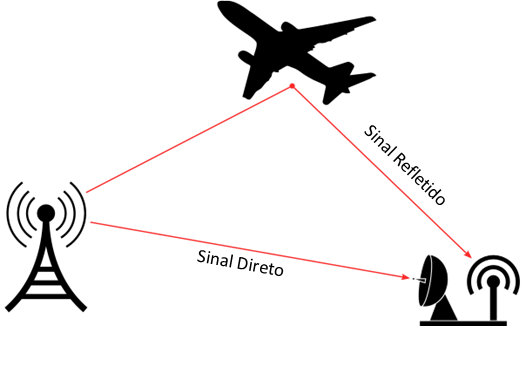
\includegraphics[scale=0.7]{chapters/ch2/assets/esquema_pcl}
\caption[Esquema Geometria Radar Passivo]{Esquema da geometria de um radar passivo}
\label{fig:esquema_pcl}
\end{figure}

O conceito do radar passivo é fazer uma relação cruzada, ou, como mais conhecido o termo, \textit{cross-correlation} entre o sinal direto e o sinal refletido em função das variáveis \textit{delay-time} que pode ser transformado em \textit{bistatic range} e o desvio de \textit{Doppler}. A \textit{cross-correlation}, de forma simples, é uma medida de similaridade entre dois sinais aplicando um atraso num deles, que neste caso, para além do atraso (\textit{delay-time}), também é feita para os diferentes \textit{Doppler}, ou seja, em duas dimensões. No entanto, na prática existem processos analíticos mais eficientes, visto que fazer a \textit{cross-correlation} a duas dimensões em tempo real torna o processo muito pesado computacionalmente.



\subsection{Geometrias Radar}
Podemos classificar os radares quanto à localização dos transmissores e recetores. O ângulo $\beta$ que estes formam, sendo o seu centro o alvo, determina o tipo de geometria \parencite{Baker2019}. Se $\beta <20^{\circ}$, o transmissor e o recetor encontram-se perto ou no mesmo sítio, então estamos perante uma geometria monostática (Figura \ref{fig:monostatic}). Quando o transmissor e recetor estão mais afastados e formam um ângulo com centro no recetor dentro dos seguintes limites, $20^{\circ}<\beta <145^{\circ}$, a geometria é bistática (Figura \ref{fig:bistatic}). Para situações particulares, em que o alvo se encontra a uma cota baixa em relação à linha imaginária que une o transmissor e o recetor ($145^{\circ}<\beta <180^{\circ}$), estamos perante uma geometria \textit{Forward Scatter} (Figura \ref{fig:fsc}).\par   

\begin{figure}[h]
\centering
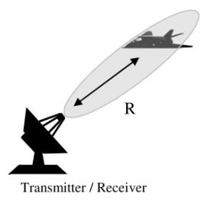
\includegraphics[scale=0.8]{chapters/ch2/assets/monostatic}
\caption[Geometria Monostática]{Geometria Monostática}
\label{fig:monostatic}
\end{figure}

\begin{figure}[h]
\centering
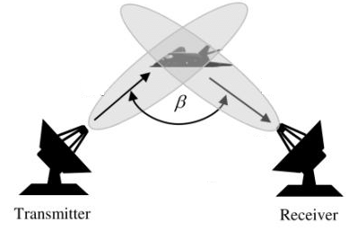
\includegraphics[scale=0.8]{chapters/ch2/assets/bistatic}
\caption[Geometria Bistática]{Geometria Bistática}
\label{fig:bistatic}
\end{figure}

\begin{figure}[h]
\centering
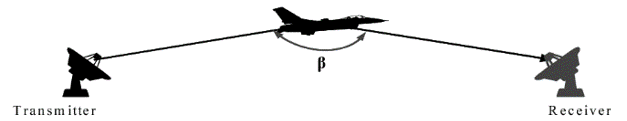
\includegraphics[scale=0.7]{chapters/ch2/assets/fsc}
\caption[Geometria \textit{Forward Scatter}]{Geometria \textit{Forward Scatter}}
\label{fig:fsc}
\end{figure}

Os radares passivos, como já discutido, têm a vantagem de não transmitirem um sinal, e ao invés usar um sinal a ser transmitido por outra fonte. Isto implica que o transmissor e o recetor não estejam no mesmo sítio nem perto, logo, quando se fala em radares passivos, assume-se uma geometria bistática.



\subsection{Alcance Bistático e \textit{Doppler}}
Como falado no ínicio deste capítulo, o alcance bistático, ou \textit{bistatic range} e o desvio de \textit{Doppler} são varáveis fundamentais para qualquer sistema radar e isso não exclui o radar passivo.\par 
O recetor bistático pode medir 3 parâmetros diferentes:
\begin{itemize}
\item A diferença em alcance entre o sinal direto e o sinal que é refletido, ou seja, o \textit{bistatic range};
\item O desvio de \textit{Doppler} do sinal recebido;
\item O ângulo $\theta_{R}$ do sinal recebido, se for usada uma antena de \textit{surveillance }direcional.
\end{itemize}

\subsubsection*{Alcance Bistático} \label{subchapter:alcance_bistatico}
Tal como representado na Figura \ref{fig:geom}, tomamos os valores $R_{T}$ como a distância do transmissor ao alvo,  $R_{R}$ como a distância do recetor ao alvo,  $\beta$ como o ângulo entre estes e com centro no alvo, e  $C$ como a distância do transmissor ao recetor, ou, \textit{Baseline}.\par


\begin{figure}[h]
\centering
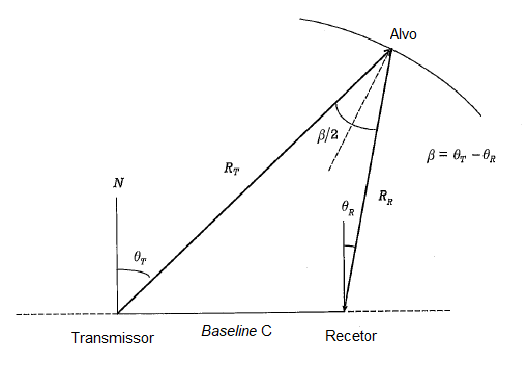
\includegraphics[scale=0.9]{chapters/ch2/assets/geom}
\caption[Parâmetros na geometria bistática]{Parâmetros na geometria bistática}
\label{fig:geom}
\end{figure}

O termo alcance bistático, ou \textit{bistatic range}, é definido em \ref{2.1}. Com este valor é possível criar elipses bistáticas (para duas dimensões) ou elipsoides bistáticos (para três dimensões) com o transmissor e o recetor como dois focos das mesmas. \par

\begin{equation} \label{2.1}
R_{T}+R_{R}-C
\end{equation}

Contudo, se a \textit{baseline} $C$ for um valor conhecido, pode-se extrair o termo \textit{range sum} $R_{T}+R_{R}$. \par
Através do conhecimento do valor de $\theta_{R}$, que é mensurável se a antena de \textit{surveillance} for direcional, a distância do alvo ao recetor é dada pela expressão \ref{2.2}.

\begin{equation} \label{2.2}
R_{R}=\dfrac{\left(  R_{T}+R_{R}\right)^{2}-C^{2}}{2\left(  R_{T}+R_{R}+C sin\theta_{R}\right)}
\end{equation}


Um dos parâmetros importantes quando se fala em alcance bistático é a \textit{range resolution}, ou seja, a resolução em alcance. Este parâmetro é definido pela capacidade de distinguir os alvos que estão muito próximos. Um bom exemplo de um sistema radar que necessite de grande \textit{range resolution} é um sistema de direção de tiro. \par 

Num radar convencional monostático, a resolução em alcance é dada por $\delta_{R}=c/2B$, onde c é a velocidade de propagação e B a largura de banda do sinal transmitido. No entanto, num radar passivo, a geometria é bistática, o que leva a existirem diferentes elipses bistáticas concêntricas, isto é, com centro no mesmo ponto, o que tem de ser tomado em conta na expressão que representa a \textit{range resolution}:

\begin{equation} \label{2.3}
\delta_{r}=\dfrac{c}{2B\left( cos\dfrac{\beta}{2}\right)}
\end{equation}

No entanto, este caso é específico para quando os dois alvos estão alinhados relativamente à bissetriz do ângulo $\beta$, como é possivel observar na figura \ref{fig:geom_varios_alvos} o exemplo dos alvos 1 e 2. Para um caso generalizado, como por exemplo o alvo 1 e o alvo 3, a expressão da \textit{bistatic range resolution} (Expressão \ref{2.4}) depende de mais um valor $\varphi$ representado na figura \ref{fig:geom_varios_alvos} como o ângulo entre o seguimento da bissetriz do ângulo $\beta$ e o segmento de reta que une o alvo 1 e o alvo 3 com centro no alvo 1. 

\begin{figure}[h]
\centering
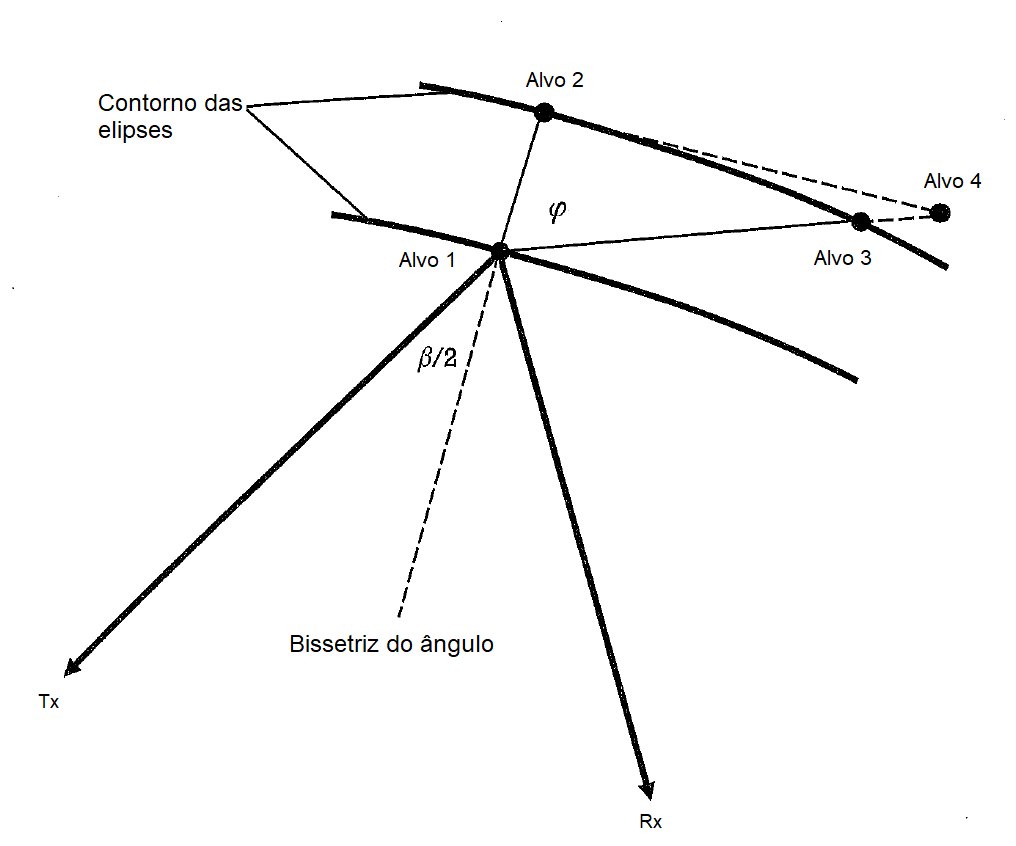
\includegraphics[scale=0.5]{chapters/ch2/assets/geom_varios_alvos}
\caption[Geometria bistática para vários alvos]{Geometria bistática para vários alvos (Adaptada da figura 2.4 \cite{Griffiths2017})}
\label{fig:geom_varios_alvos}
\end{figure}


\begin{equation} \label{2.4}
\delta_{r}=\dfrac{c}{\left[ 2B\left( cos\dfrac{\beta}{2}\right)\right] cos\varphi}
\end{equation}


A expressão do \textit{bistatic range resolution} permite interpretar a geometria bistática quanto à distância entre o transmissor e recetor. Da expressão \ref{2.4} conclui-se que quanto mais o ângulo $\beta$ se aproxima de um ângulo reto, o denominador tende para um valor próximo de 0, ou seja, a resolução em alcance torna-se fraca. Contudo, nesta situação estamos perante uma geometria \textit{forward scatter}, discutido no inicio deste capítulo, o que pode ser contornando usando vários recetores em locais diferentes.\par 
Para radares passivos, continuando a interpretação da expressão \ref{2.4}, os iluminadores de oportunidade mais utilizados têm pouca largura de banda $B$, o que se reflete numa resolução em alcance mais reduzida. No entanto, os sinais de DVB-T, discutidos no Capítulo \ref{chap:Chapter1}, têm uma largura de banda na ordem dos 8 MHz, o que já permite uma resolução em alcance na ordem dos 40m.

\subsubsection*{\textit{Doppler}} 
Ignorando efeitos relativisticos, o desvio de \textit{Doppler} bistático ocorre quando pelo menos um dos elementos transmissor, alvo, recetor se encontra em movimento. É definido como a taxa de variação temporal do comprimento total do caminho percorrido pelo sinal refletido, normalizado pelo comprimento de onda $\lambda$ \parencite{Willis2005}.  No caso mais comum, em que apenas o alvo se encontra em movimento, o desvio de \textit{Doppler} é dado por \parencite{Willis2005},

\begin{equation} \label{2.5}
f_{D}=\dfrac{2v}{\lambda}cos\delta cos\left( \dfrac{\beta}{2}\right) 
\end{equation}

onde $\delta$ é o ângulo formado pelo sentido do vetor velocidade $v$ e a bissetriz do ângulo $\beta$ com centro no alvo. \par

Na equação \ref{2.5}, quando $\beta =180^{\circ}$, estamos perante uma geometria \textit{forward scatter} e temos um valor de desvio de \textit{Doppler} $f_{D}=0$ para todos os ângulos de $\delta$. Quando $\beta =0^{\circ}$, fica-se reduzido a uma geometria monostática. 


A resolução de \textit{Doppler} no radar bistático é semelhante à resolução de \textit{Doppler} no radar monostático, isto porque depende do tempo de integração $T$ que é um parâmetro escolhido e indiferente à geometria do radar. Quanto maior for o tempo de integração, melhor é a resolução de \textit{Doppler}. A expressão \ref{2.6} define o requisito mínimo entre a separação dos alvos.

\begin{equation} \label{2.6}
\vert f_{a1}-f_{a2}\vert = \dfrac{1}{T}
\end{equation}

sendo que $f_{a1}$ e $f_{a2}$ são os desvios de \textit{Doppler} para cada alvo, definidos em \ref{2.5}. Substituindo as equações dos alvos em \ref{2.5} na equação \ref{2.6}, e resolvendo em ordem a $\Delta v$, ou seja, a diferença entre os dois vetores velocidade projetados na bissetriz do ângulo $\beta$ ($\Delta v=\left( v_{1}cos\delta_{1}-v_{2}cos\delta_{2}\right) $), vem,

\begin{equation} \label{2.7}
\Delta v = \dfrac{\lambda}{2T\cdot cos\left( \beta /2\right) }
\end{equation}

Com esta expressão, assumimos que os alvos partilham a mesma bissetriz, o que na realidade é pouco provável. No entanto, esta restrição pode ser ignorada, se,
\begin{enumerate}
	\item A separação entre os alvos não for suficiente para permitir resolução em \textit{range};
	\item O ângulo entre as bissetrizes dos dois alvos é pequeno.
\end{enumerate}



\subsection{Previsão de \textit{Performance}}
Para qualquer sistema radar é importante conseguir prever com precisão os vários aspetos da \textit{performance} do sistema. O ponto de início de uma análise de \textit{performance} mi, radar passivo é a equação de radar bistática, falada brevemente no capítulo \ref{chap:Chapter3} e rescrita  de uma forma que reflete as caraterísticas do radar \gls{PCL} para o caso da geometria bistática vem \parencite{Griffiths2005},

\begin{equation} \label{2.8}
\dfrac{P_{r}}{P_{n}}= \dfrac{P_{t}G_{t}}{4\pi r^{2}_{1}}\cdot\sigma_{b}\cdot\dfrac{1}{4\pi r^{2}_{2}}\cdot\dfrac{G_{r}\lambda^{2}}{4\pi}\cdot\dfrac{1}{kT_{0}BF}\cdot L 
\end{equation}

onde,\par
$P_{r}$: "potência do sinal recebido"\par
$P_{n}$: "potência do ruído do recetor"\par
$P_{t}$: "potência do sinal transmitido"\par
$G_{t}$: "ganho da antena de transmissão"\par
$G_{r}$: "ganho da antena de receção"\par
$r_{1}$: "alcance do transmissor ao alvo"\par
$r_{2}$: "alcance do recetor ao alvo"\par
$\sigma_{b}$: "\gls{RCS} bistática do alvo"\par
$\lambda$: "comprimento de onda do sinal"\par
$k$: "constante de \textit{Boltzmann}$ =1,380649x10^{-23} J\cdot K^{-1}$"\par
$T_{0}$: "temperatura de ruído de referência, $290K$"\par
$B$: "largura de banda efetiva do recetor"\par
$F$: "\textit{noise figure}\footnote{\textit{noise figure} ou figura de ruído representa a diferença em $dB$ entre o ruído de entrada do recetor e a ruído de saída do mesmo} efetiva do recetor"\par
$L(\leq 1)$: "perdas do sistema"\par
 
É de notar que para esta equação, usada para a previsão de \textit{peformance}, é importante conhecer o valor de cada parâmetro a ser usado, o que leva a ter uma ideia bem definida da função do sistema radar e o que se pretende com o mesmo. Também é necessário um conhecimento dos vários iluminadores de oportunidade e as suas caraterísticas, falado no subcapítulo \ref{IOS}.\par 


\subsubsection*{Potência transmitida}
A potência transmitida $P_{t}$ é substancial para muitas das fontes de sinal para o radar passivo devido aos recetores de sinais de \textit{broadcast} e comunicações apresentarem, normalmente, antenas ineficientes e com \textit{noise figures} baixas. Isto é, as antenas de receção dos sinais mais comuns no espetro, são antenas que têm de ser relativamente baratas, por exemplo uma antena de receção de \gls{DVB-T} ou de receção de radiodifusão sonora em \gls{VHF}, de forma a o utilizador comum poder ter acesso a qualquer uma destas, logo este tipo de antenas são mais ineficientes e isso é colmatado por uma maior potência de transmissão por parte da estação de difusão.\par 
Seja qual for o iluminador de oportunidade utilizado, a potência do transmissor implica com a densidade de potência $\Phi =(P_{t}G_{t})/4\pi r^{2}_{1}$, que é uma caraterística importante na escolha da fonte de sinal a ser utilizada. 

\subsubsection*{\gls{RCS} bistática do alvo}
Na deteção de alvos usando radares \gls{PCL}, a \gls{RCS} bistática do alvo é uma caraterística importante na previsão de \textit{performance}. As caraterísticas do alvo definem este parâmetro e também a sua localização em relação ao transmissor - recetor, formando o ângulo bistático $\beta$, falado no ínicio deste capítulo. É dificil ter uma previsão deste parâmetro, mas há um caso especial a ser considerado, que é para uma geometria \textit{forward scatter}. \par 
Quando o ângulo bistático, representado na figura \ref{fig:geom} por $\beta$, toma valores próximos de $180^{\circ}$, entra-se na região de \textit{forward scatter} e nesta zona, o valor da \textit{cross-section} do alvo é melhorado devido ao principio de \textit{Babinet}. Este principio aplicado a este caso, diz que para um alvo que é um absorvedor perfeito, na região de \textit{forward scatter}, a dispersão de energia que é transmitida para o recetor é igual à dispersão que era transmitida se no lugar deste alvo estivesse presente uma abertura com a mesma forma \parencite{Griffiths2005}. Assim sendo, para um alvo com uma área transversal $A$, a \gls{RCS} é representada na equação \ref{2.9} e a largura de feixe do sinal refletido na equação \ref{2.10}.

\begin{equation} \label{2.9}
\sigma_{b}=\dfrac{4\pi A^{2}}{\lambda^{2}}
\end{equation}

\begin{equation} \label{2.10}
\theta_{b}=\dfrac{\lambda}{d}
\end{equation}

Onde $d$ é a dimensão linear no plano apropriado.
Ao analisar as duas funções fazendo variar a frequência (a partir da figura \ref{fig:rcs_ang}) é de notar que com menor frequência consegue-se menor largura de feixe e maior \gls{RCS} bistática do alvo. Isto fundamenta o uso de radares com frequência baixa para a deteção na zona de \textit{forward scatter}.

\begin{figure}[h]
\centering
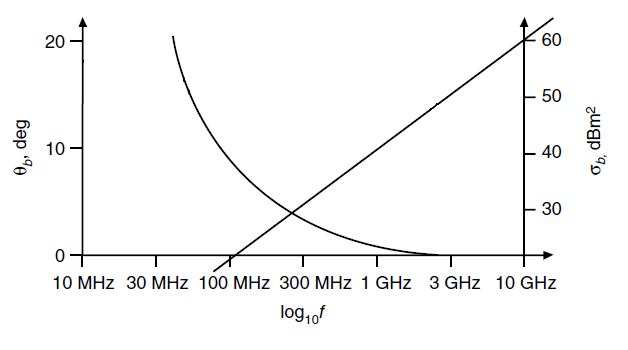
\includegraphics[scale=0.7]{chapters/ch2/assets/rcs_ang}
\caption[Variação da \gls{RCS} e largura de feixe consoante a frequência]{Variação da \gls{RCS} e largura de feixe consoante a frequência, para um alvo de $10m^{2}$ de área e dimensão linear $20m$ (figura 1 \cite{Griffiths2005})}
\label{fig:rcs_ang}
\end{figure}

\subsubsection*{\textit{Noise figure} do recetor}
A \textit{noise figure} , de uma forma simples, é definida pela relação entre a \gls{SNR} à entrada do recetor e a \gls{SNR} à saída do mesmo, ou seja, é um valor que representa o desempenho do recetor, sendo que quanto menor for, mais perto se encontram os dois valores de \gls{SNR} e consequentemente melhor desempenho.\par
Não é só a \textit{noise figure} que contribui para os níveis de ruído presentes no sinal. Por forma a compreender melhor os fatores que contribuem para os níveis de ruído, pode ser criada uma função $P_{i}(\theta ,f)$ dependente da direção e frequência que engloba todos estes fatores, sendo estes:
\begin{enumerate}
\item \textit{Noise figure} do recetor;
\item Sinal direto do transmissor, que é a componente mais forte desta função;
\item Componente de \textit{multipath}, ou seja, todas as réplicas do sinal direto atrasadas no tempo devido a reflexões em obstáculos;
\item Sinal direto e \textit{multipath} de outros sinais que possam estar a transmitir no mesmo canal;
\item Outros sinais devido a fontes diversas, como por exemplo radiação de dispositivos eletrónicos.
\end{enumerate}
Devido a todas estas componentes é necessário haver um cancelamento das mesmas de forma a ser percetível o sinal refletido no alvo e aumentar a sensibilidade e alcance do sistema. No capítulo \ref{chap:Chapter4} é abordado este assunto com mais pormenor.\par 

A \textit{noise figure} do recetor, pode ser representada pela seguinte equação,

\begin{equation} \label{2.11}
NF=10log_{10}\left( \dfrac{SNR_{i}}{SNR_{o}}\right)=SNR_{i,dB}-SNR_{o,dB}
\end{equation}

\subsubsection*{Ganho de integração}
A largura de banda efetiva do recetor $B$, que é normalmente a largura de banda do sinal transmitido, é adaptada ao sinal direto e, quando combinada com um tempo de integração $T$, resulta um ganho de integração como representado na equação \ref{2.12}. Este tempo de integração é referido no capítulo \ref{chap:Chapter4} como o tempo em que é integrada a \textit{cross-correlation}.

\begin{equation} \label{2.12}
G_{i}=BT
\end{equation}

Para o caso da \gls{DVB-T}, que a largura de banda é aproximadamente $8 MHz$, com um tempo de integração de 1 segundo dá um ganho de processamento $G_{i}$ de $69dB$, o que se torna muito melhor que o ganho de integração de por exemplo uma transmissão rádio \gls{FM} com uma largura de banda de $50 kHz$, que para 1 segundo de tempo de integração vem um ganho de $47dB$.\par 
Tendo como referência a equação \ref{2.12}, podemos ter a perceção de que para obter maior ganho de integração num determinado sinal, basta aumentar o tempo de integração da correlação para valores maiores, o que é verdade, mas ao fazer isto, existem vários efeitos limitativos que vão ocorrer. Um dos principais e efeito mais limitativo é conhecido como \textit{target flutuations}, ou seja, alterações repentinas da força do sinal, que é resultante de maioritariamente dois fatores: a mudança de ângulo de observação e o efeito de \textit{multipath}. Com isto, a função do ganho de integração já não vai ser linear e aumentar sempre com o aumento do tempo de integração, pelo oposto, dependendo de vários fatores vai ter um pico para um determinado tempo de integração.\par 
Este tema tem sido estudado e foram tiradas várias conclusões com resultados de alvos reais \parencite{Malanowski2008}. Uma das conclusões que foi verificada, foi que o tempo de integração da correlação é importante para ecos fracos, que são originados por reflexões em alvos distantes e que para alvos mais próximos, normalmente existe boa \gls{SNR} e não é necessário maior tempo de integração. Também são abordadas e testadas soluções para este problema usando diferentes versões da função de correlação.

\subsubsection*{Previsão de \textit{performance} na deteção}
Como conclusão deste subcapítulo e depois da abordagem em alguns tópicos considerados mais importantes na previsão de \textit{performance} de um radar passivo são apresentados exemplos práticos \parencite{Griffiths2005} de uma previsão de alcance para dois transmissores de rádio \gls{FM} localizados em Wrotham e Crystal Palace, com o recetor localizado no edifício \textit{Engineering Sciences Faculty} da \gls{UCL}.

\begin{figure}[h]
\centering
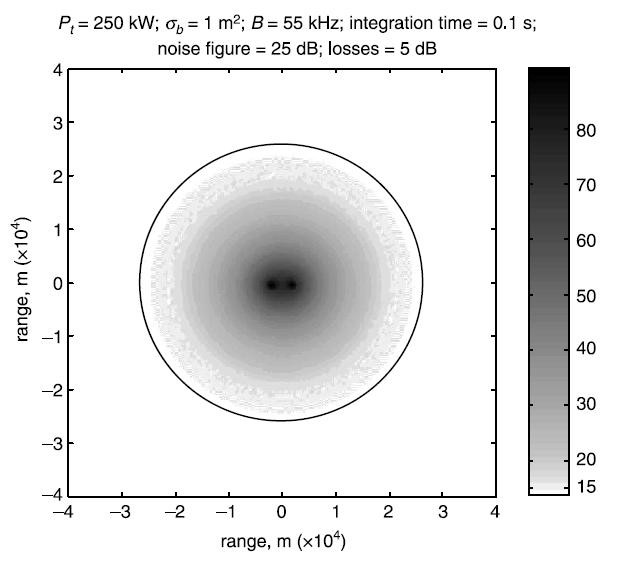
\includegraphics[scale=0.6]{chapters/ch2/assets/wrotham}
\caption[Alcance de deteção para um transmissor em Wrotham e recetor na \gls{UCL}]{Alcance de deteção para um transmissor em Wrotham e recetor na \gls{UCL} (figura 3 \cite{Griffiths2005})}
\label{fig:wrotham}
\end{figure}

\begin{figure}[h]
\centering
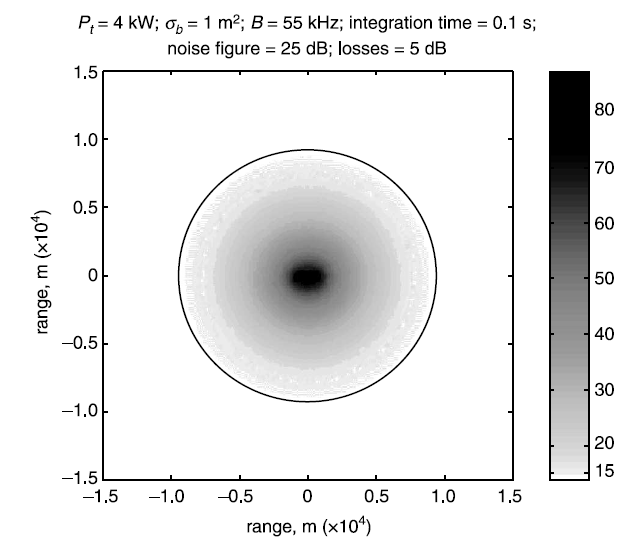
\includegraphics[scale=0.6]{chapters/ch2/assets/cp}
\caption[Alcance de deteção para um transmissor em Crystal Palace e recetor na \gls{UCL}]{Alcance de deteção para um transmissor em Crystal Palace e recetor na \gls{UCL} (figura 4 \cite{Griffiths2005})}
\label{fig:cp}
\end{figure}

Várias observações podem ser feitas com estas duas figuras, mas a primeira que salta à vista é o alcance de deteção para um transmissor, sendo que a linha preta que contorna os dois transmissores é uma referência para os $15dB$, que ronda pouco mais de $10km$ para o transmissor em Crystal Palace, e para o transmissor em Wrotham o já está na ordem dos $30km$. Isto deve-se à potência de transmissão, que no caso de Crystal Palace é de $4kW$ e em Wrotham, $250kW$, o que leva de novo a um dilema que tem sido debatido ao longo desta dissertação, que é a escolha do iluminador de oportunidade e a variedade de fatores que afetam esta escolha nunca conseguindo ter uma fonte de sinal ideal, mas sim uma mais adaptada à função do radar passivo.


\subsection{Formação de Imagem}
O radar \gls{PCL}, ou radar passivo, não oferece apenas a capacidade de explorar os iluminadores de oportunidade para o fim de deteção e localização, mas também para a formação de imagens. Tem muitas vantagens na utilização deste tipo de radares para este fim, sendo um bom exemplo o mapeamento de uma zona com qualquer condição meteorológica e sem transmitir nenhum sinal.\par 
O objetivo deste subcapítulo é dar um conhecimento superficial sobre uma das capacidades dos radares passivos e dar a conhecer alguns conceitos fundamentais e um algoritmo \gls{PB-ISAR} na formação de imagens.\par 

\subsubsection*{\gls{ISAR}}
O conceito do \gls{ISAR} é utilizar uma configuração de um radar de abertura sintética, mas em que o radar esteja estático e o alvo em movimento em relação ao mesmo (Inverso do \gls{SAR}). Ao utilizar esta abordagem é necessário criar uma abertura sintética por forma a ter boa resolução \textit{cross-range}, que é conseguida, no caso do \gls{SAR}, por um elemento que se move ao longo de uma trajetória conseguindo assim meios para formar uma matriz virtual para o intervalo de tempo em que esteve a observar. O único caso em que esta matriz virtual criada pela abertura sintética é diferente de uma imagem obtida por uma matriz real é quando o espaço a ser iluminado está estático em relação ao radar durante a formação da mesma.\par 
Os elementos chave para a construção de uma imagem usando \gls{ISAR} são \parencite{Martorella2019}:

\begin{enumerate}
\item Utilizar um sinal com grande largura de banda por forma a ter uma boa resolução em \textit{range} $\delta_{R}$ falado no subcapítulo \ref{subchapter:alcance_bistatico} para o caso monostático e bistático.

\item Processar os ecos recebidos durante o tempo de observação em diferentes ângulos de incidência no alvo a iluminar. A resolução \textit{cross-range} é definida na equação \ref{2.13}, que é inversamente proporcional à variação de ângulo de incidência $\Delta$.
\begin{equation} \label{2.13}
\delta_{cr}=\dfrac{c}{2f_{0}\Delta}
\end{equation}
\end{enumerate}

Por forma a compreender o processo de formação de imagem de uma forma simples, segue-se o diagrama de blocos da figura \ref{fig:img}. Este diagrama não compreende todos os processos englobados na formação de imagem através de \gls{ISAR}, mas apenas os fundamentais para uma breve explicação que é o objetivo deste subcapítulo.

\begin{figure}[h]
\centering
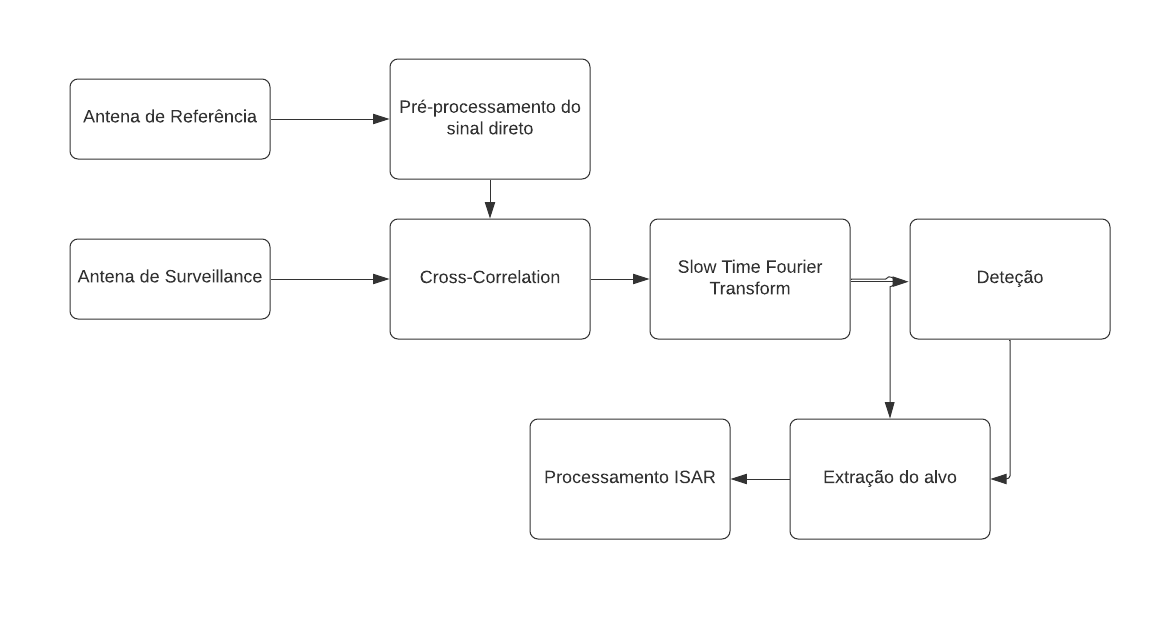
\includegraphics[scale=0.8]{chapters/ch2/assets/img}
\caption[Diagrama de blocos ISAR]{Diagrama de blocos ISAR}
\label{fig:img}
\end{figure}

Depois de recebido o sinal da antena de referência e \textit{surveillance} o sinal direto é submetido a um pré processamento explicado no capítulo \ref{chap:Chapter4} que para o caso de \gls{DVB-T} visto que é um dos iluminadores de oportunidade com maior largura de banda o que permite maior resolução em \textit{range}, reconstrução e equalização do sinal. Esse sinal direto passa por um equivalente a um filtro adaptado, ou seja, a \textit{cross-correlation} do sinal direto com o sinal refletido no alvo.\par 

O \textit{input} do algoritmo \gls{PB-ISAR} é um mapa \textit{range-Doppler} que contém o eco do alvo mais \textit{clutter} e ruído. No entanto, os radares do tipo \gls{ISAR} são desenvolvidos para trabalhar no domínio frequência/\textit{slow-time} ou \textit{range}/\textit{slow-time} e para isso ser possível é necessário transformar os dados recebidos do mapa \textit{range-Doppler} num destes domínios. Uma das formas para o fazer, no caso de transformar no domínio frequência/\textit{slow-time} é aplicar uma transformada de \textit{Fourier} inversa à imagem em \textit{range-Doppler} do alvo.\par 

Após este processamento, que no caso do filtro adaptado é explicado sucintamente no capítulo \ref{chap:Chapter4}, o sinal passa por um bloco de extração do alvo que consiste em quatro passos:
\begin{enumerate}
\item processo de \textit{clustering} dos alvos detetados no mapa \textit{range-Doppler} com um exemplo representado na imagem \ref{fig:cluster};

\begin{figure}[h]
\centering
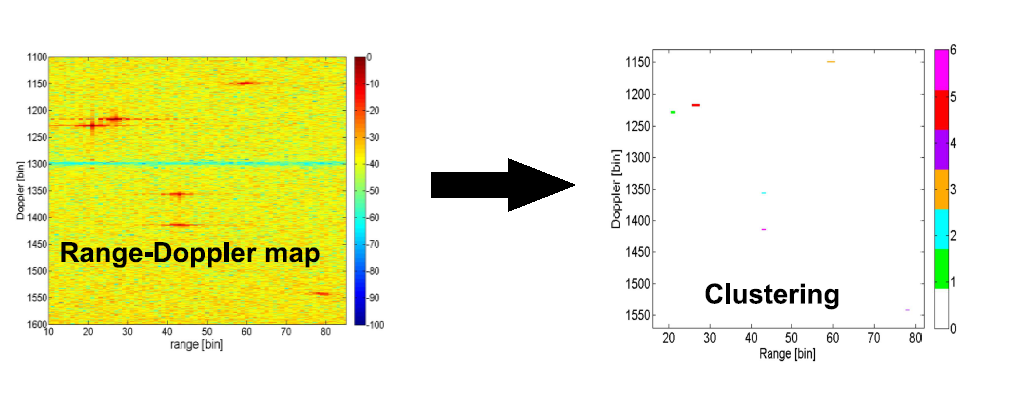
\includegraphics[scale=0.6]{chapters/ch2/assets/cluster}
\caption[Processo de \textit{clustering}]{Processo de \textit{clustering} (adaptado da figura do slide 36 da apresentação do artigo \cite{Martorella2019})}
\label{fig:cluster}
\end{figure}

\item criação de uma caixa em redor do alvo;
\item através das caixas formadas em redor dos alvos, resolver possíveis problemas de \textit{overlapping} e desviar erros de deteção de vários alvos próximos quando na realidade apenas se encontra um;
\item extração dos alvos detetados.
\end{enumerate}

De seguida a imagem passa por um pré-processamento do \gls{ISAR} por forma a definir perfis de \textit{range} em cada alvo extraído que, por fim, é submetida ao processamento do \gls{ISAR} onde é feito uma estimativa a partir do pré-processamento da posição dos alvos em relação ao recetor e, posteriormente uma compensação do movimento do alvo seguida de uma \gls{DFT} para obter a imagem \gls{ISAR} do alvo. Para um entendimento mais profundo dos cálculos e processamento, tanto como resultados obtidos com este métodos há vários trabalhos que se podem consultar como \cite{Martorella2019}.
% Chapter 3

\chapter{Teoria de Antenas} % Main chapter title
\label{chap:Chapter3} % For referencing the chapter elsewhere, use \ref{chap:Chapter3} 

%----------------------------------------------------------------------------------------
\section{Teoria Básica de Antenas}
Uma antena é definida como "um dispositivo geralmente metálico (com haste ou fio) para irradiar ou receber ondas de rádio" \parencite{Balanis2016}, ou seja, uma antena, é o dispositivo que permite a transição entre o meio que a rodeia e o equipamento, que se pode observar na Figura \ref{fig:antena transicao}. 
Este dispositivo é um transdutor que converte energia elétrica em ondas eletromagnéticas ou vice versa, sendo que é uma antena de transmissão, se converter um sinal elétrico num sinal eletromagnético e é uma antena de receção, se converter um sinal eletromagnético em sinal elétrico. 

\begin{figure}[h]
\centering
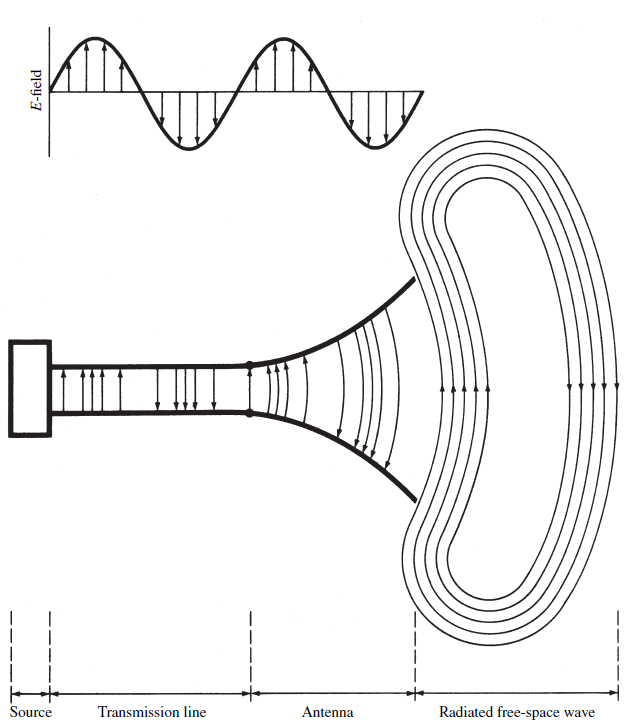
\includegraphics[scale=0.6]{chapters/ch3/assets/Antenna_transicao}
\caption[Antena como meio de transição]{Antena como um meio de transição (Figura 1.1 - \cite{Balanis2016})}
\label{fig:antena transicao}
\end{figure}

\subsection{Tipos de Antenas}
Neste subcapítulo irá ser introduzido de uma forma breve, os vário tipos de antenas, a sua utilização e vantagens entre estes. 

\subsection*{Antenas de Fio}
Estas antenas são umas das mais antigas, que apresentam uma configuração mais simples, como se pode observar na Figura \ref{fig:wire antenna}, sendo apenas constituídas por um fio que pode variar na sua dimensão e na sua forma e ainda podem ser utilizadas nas mais variadas aplicações. Podem tomar uma forma aleatória, desde um fio direito (dipolo) até um fio com as mais diversas formas. \par 
As antenas de fio podem ser encontradas nos mais variados locais, desde aeronaves, carros ou navios a edifícios.

\begin{figure}[h]
\centering
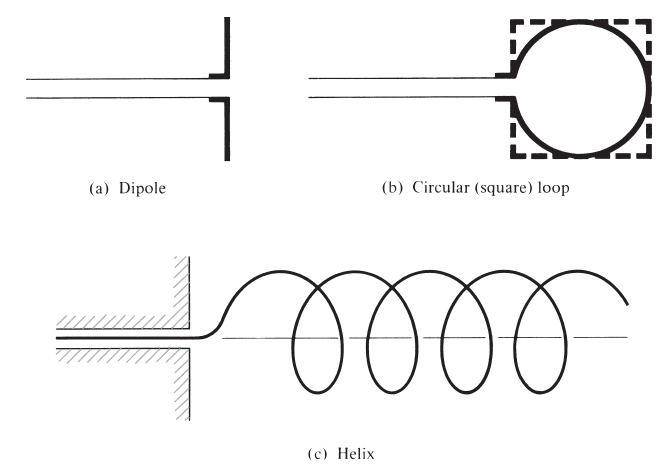
\includegraphics[scale=0.6]{chapters/ch3/assets/wire_antenna}
\caption[Antena de Fio]{Exemplos de vários tipos de antenas de fio (Figura 1.3 - \cite{Balanis2016})}
\label{fig:wire antenna}
\end{figure}

\subsection*{Antenas de Abertura}
Os campos no fim de um guia de ondas aberto não são uniformes devido a esta mesma abertura, assim, para este caso, assume-se que os campos são iguais a como se o guia de ondas continuasse fechado. As antenas de abertura entram quando se pretende aumentar a diretividade à saída do guia, abrindo as extremidades do mesmo de forma a dar uma forma como se observa na Figura \ref{fig:aperture antenna2}. Este tipo de antenas, em especifico as antenas de abertura piramidais, são utilizadas para alimentar ou calibrar grandes antenas de prato.\par
Assim sendo, as antenas de abertura são utilizadas para frequências mais elevadas, especificamente em frequências de micro-ondas e podem ser aplicadas nas mais variadas formas geométricas, como retangulares, elípticas, circulares, piramidais, entre outras.

\begin{figure}[h]
\centering
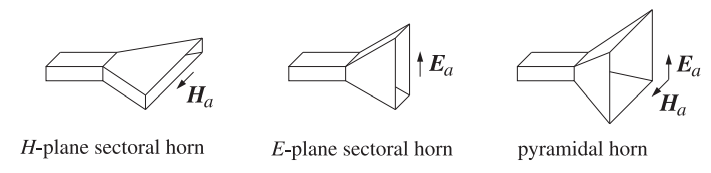
\includegraphics[scale=0.6]{chapters/ch3/assets/aperture_antenna2}
\caption[Antena de Abertura]{Antenas de abertura no plano H, E e piramidal}
\label{fig:aperture antenna2}
\end{figure}


\subsection*{Antenas de \textit{Microstrip}}
Uma antena \textit{microstrip}, conhecida como antena impressa, é um tipo de antena que está inserida numa placa de circuito impresso e funciona como uma antena interna.\par
Hoje em dia são utilizadas em aplicações comerciais, tendo como as suas maiores vantagens o facto de serem baratas e simples de manufaturar e apresentarem um tamanho reduzido. Este tipo de antenas são aplicadas em frequências \gls{UHF}.\par 
A sua construção consiste num \textit{patch} metálico sobre um substrato. Este \textit{patch} pode apresentar as mais variadas formas como representado na Figura \ref{fig:microstrip}, sendo as retangulares e circulares as mais comuns. Têm ainda as vantagens de serem impressas em superfícies com as mais variadas formas, sendo robustas e versáteis nos parâmetros da sua frequência de ressonância, polarização e impedância (\cite{Balanis2016}).

\begin{figure}[h]
\centering
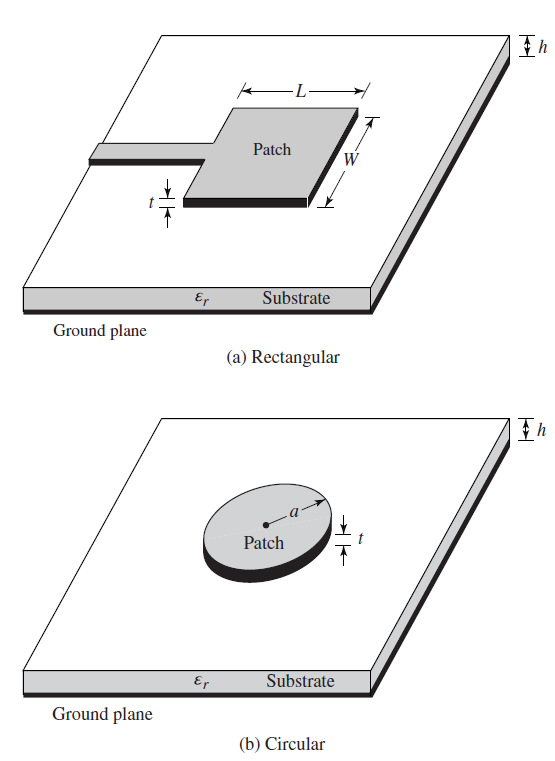
\includegraphics[scale=0.6]{chapters/ch3/assets/microstrip}
\caption[Antena \textit{Microstrip}]{Exemplos de duas configurações de \textit{patches} diferentes (Figura 1.5 - \cite{Balanis2016})}
\label{fig:microstrip}
\end{figure}

\subsection*{Antenas de Matrizes}
As antenas de matrizes surgem nas aplicações em que é necessário mais que um elemento. Consegue-se assim agrupar vários elementos de forma a obter as características pretendidas. Algumas alterações às caraterísticas que se conseguem com este tipo de antenas antenas são o aumento de ganho, alterar o diagrama de radiação, determinar a direção de chegada de um sinal ou maximizar o \gls{SINR}\footnote{\gls{SINR} é um indicador de qualidade de transmissão ajustado a comunicações móveis devido à interferência de outros utilizadores ser mais significativa \parencite{Jeske2004}.}.

\subsection*{Antenas de Lente}
Este tipo de antenas utiliza as propriedades de convergência e divergência das lentes para a receção ou transmissão de sinal. O tamanho da lente a ser utilizada depende da frequência - quanto maior for a frequência, menor a lente. Dito isto, é mais favorável usar este tipo de antenas em frequências mais altas, visto que a lente será menor. As suas aplicações são semelhantes às das refletoras parabólicas, especificamente quando usadas em frequências mais altas e que necessitem de mais largura de banda.

\subsection*{Antenas Refletoras}
As antenas refletoras existem desde o final do século XIX, no entanto começaram a ser aplicadas em radares na Segunda Guerra Mundial e a partir do final do século XX em comunicações espaciais. Estas aplicações devem-se à sua capacidade de transmissões a grandes distâncias. Podem-se apresentar nas mais diversas formas, como plano refletor, refletor curvilíneo, entre outros.\par 
O seu modo de funcionamento baseia-se na convergência da energia numa direção como demonstrado na Figura \ref{fig:reflector}, o que leva, para além de um grande alcance, a uma grande diretividade.

\begin{figure}[h]
\centering
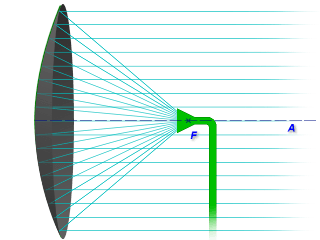
\includegraphics[scale=0.6]{chapters/ch3/assets/reflector}
\caption[Antena Refletora]{Funcionamento de uma Antena Refletora}
\label{fig:reflector}
\end{figure}

\subsection{Parâmetros Fundamentais}
Neste subcapítulo vão ser discutidos os parâmetros mais relevantes que estão relacionados com o funcionamento de uma antena e com a sua \textit{performance}. Grande parte dos parâmetros estão definidos no IEEE 1983 Standard Definitions for Antennas and Propagation.

\subsection*{Diagrama de Radiação}
Um diagrama de radiação é a função ou representação gráfica que descreve as propriedades espaciais de radiação de uma antena. É de extrema importância conhecer este padrão de radiação de uma antena e poder controla-lo, visto que a distribuição de energia eletromagnética, se for mal dimensionada, pode comprometer o projeto. \par 

A manipulação do diagrama de radiação de uma antena é dependente do objetivo da mesma. Podemos ter como finalidade um diagrama de radiação que seja direcional (Figura \ref{fig:direcional}), como numa ligação ponto a ponto, ou podemos como finalidade, um diagrama de radiação omnidirecional (Figura \ref{fig:omnidirecional}), ou seja, que radia, idealmente, com igual intensidade para todas as direções.\par

Para este efeito são utilizadas coordenadas esféricas ($r$, $\varphi$ e $\theta$), sendo que a antena se encontra na origem do referencial. A propriedade mais relevante nos diagramas de radiação é a distribuição espacial, em duas ou três dimensões, da energia radiada em função da posição do observador de acordo com um azimute ($\theta$ constante).\par 

\begin{figure}[h]
\centering
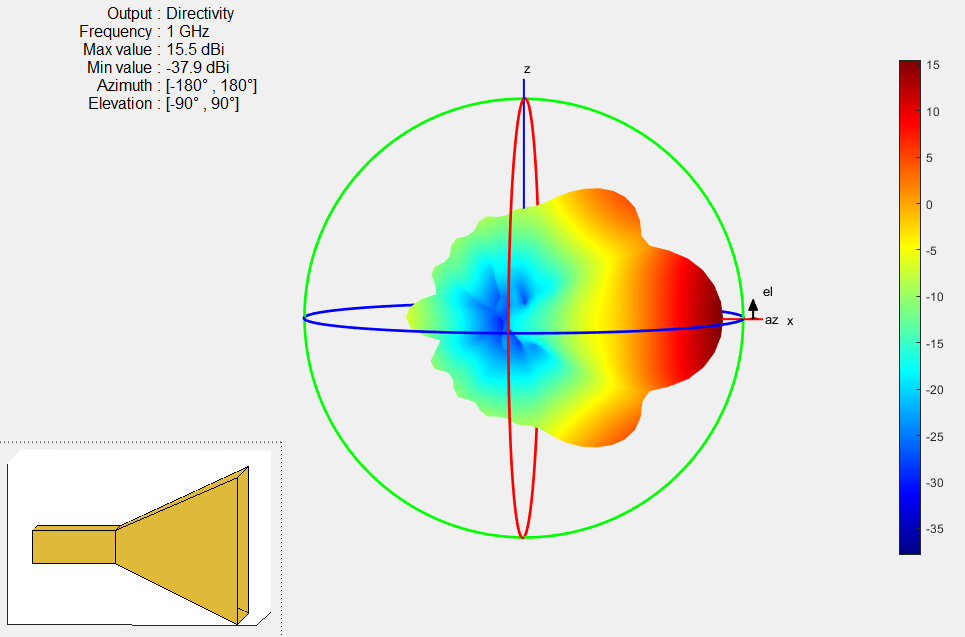
\includegraphics[scale=0.6]{chapters/ch3/assets/matlab_ad1}
\caption[Diagrama de radiação direcional]{Diagrama de radiação direcional - Corneta de guia de ondas dimensionada para 1GHz (MATLAB Antenna Designer Toolkit)}
\label{fig:direcional}
\end{figure}

\begin{figure}[h]
\centering
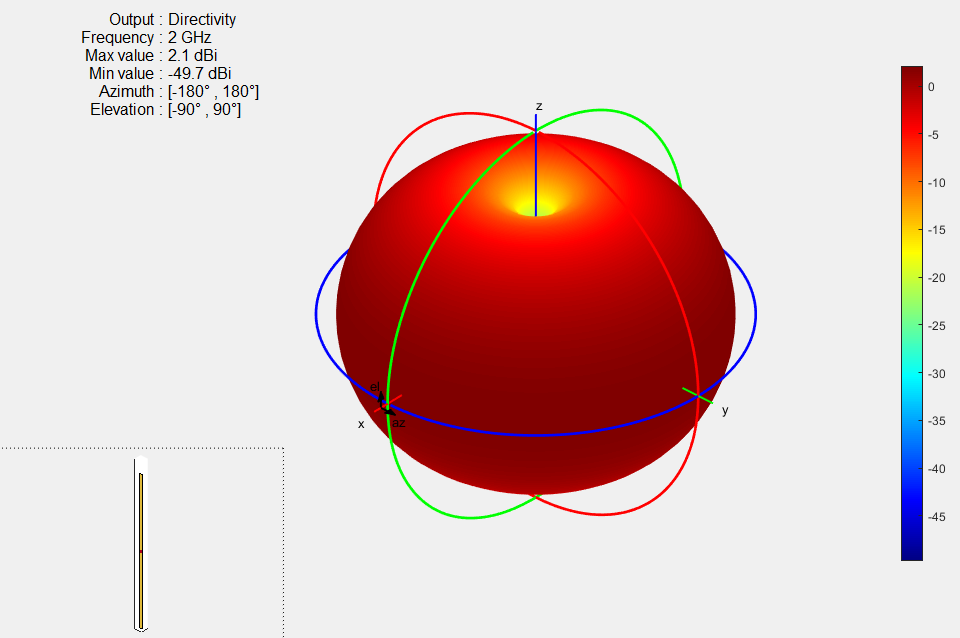
\includegraphics[scale=0.6]{chapters/ch3/assets/matlab_ad2}
\caption[Diagrama de radiação omnidirecional]{Diagrama de radiação omnidirecional - Dipolo dimensionado para 2GHz (MATLAB Antenna Designer Toolkit)}
\label{fig:omnidirecional}
\end{figure}

Os lóbulos são um dos parâmetros fundamentais de um diagrama de radiação, que representam a energia radiada numa direção relativamente ao transmissor e podem ser classificados em lóbulos principais, secundários, laterais e posteriores (Figura \ref{fig:elem_carat_dg}). O lóbulo principal é o lóbulo que contém a direção da radiação máxima, que no caso da Figura \ref{fig:elem_carat_dg}, está definido no sentido do eixo dos zz. Os lóbulos secundários são todos os lóbulos expecto o principal. Os lóbulos laterais são todos os que radiam energia para qualquer direção que não seja a pretendida. Os lóbulos posteriores contêm a energia que é radiada num ângulo de 180$^{\circ}$ em relação à direção do feixe da antena. \par 

A largura de feixe a meia potência (\gls{HPBW}) e a largura de feixe ao primeiro nulo (\gls{FNBW}) estão relacionadas com a capacidade de resolução da antena, ou seja, a sua capacidade de distinguir dois alvos. O critério para distinguir dois alvos é que a \gls{HPBW} seja aproximadamente \gls{FNBW}/2, isto é, se dois alvos estiverem separadas por distâncias angulares iguais ou superiores a \gls{HPBW}$\approx$\gls{FNBW}/2 de uma antena, esta consegue distingui-los \parencite{Kraus1988}. Os fatores que afetam a largura de feixe são o comprimento de onda ($\lambda$), a forma do diagrama de radiação e as dimensões da antena. \par 

\begin{figure}[h]
\centering
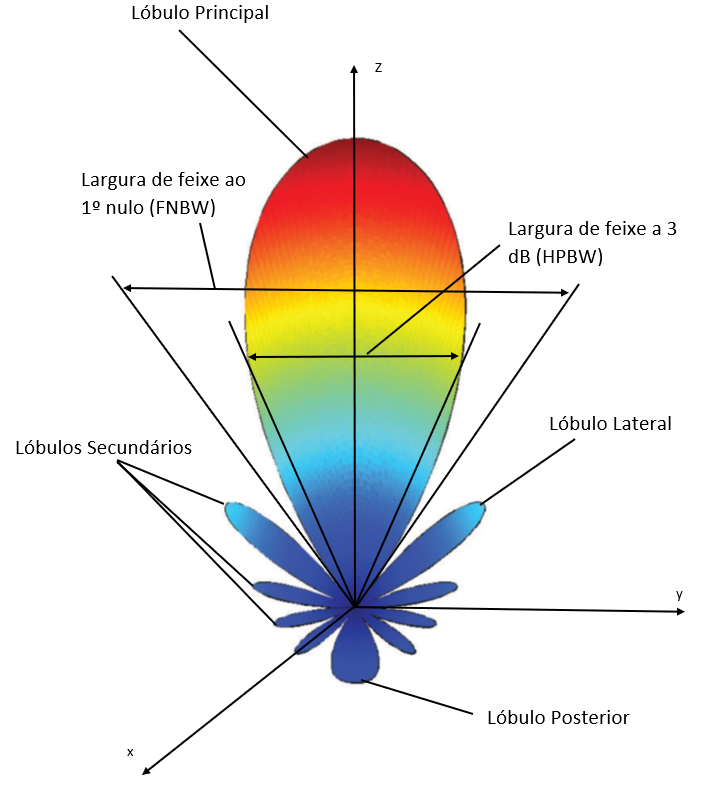
\includegraphics[scale=0.6]{chapters/ch3/assets/elem_carat_dg}
\caption[Elementos caraterísticos do diagrama de radiação]{Elementos caraterísticos do diagrama de radiação}
\label{fig:elem_carat_dg}
\end{figure}

Os diagramas de radiação podem ser classificados quanto à diretividade em que as antenas radiam. Um radiador isotrópico é definido com uma antena hipotética e sem perdas que radia igualmente em todas as direções e é normalmente tomado como referência para exprimir a diretividade de antenas. o radiador direcional é caracterizado por radiar ondas eletromagnéticas em determinadas direções e o radiador omnidirecional radia energia de igual forma em todas as direções \parencite{Balanis2016}.

\subsubsection*{Planos Principais}
Para antenas com polarização linear, discutido com mais detalhe no subcapítulo Polarização, consideram-se os seguintes planos:
\begin{itemize}
\item Plano E: Definido pelo plano que contém o vetor do campo elétrico e a direção da máxima radiação;
\item Plano H: Definido pelo plano que contém o vetor do campo magnético e a direção da máxima radiação.
\end{itemize}
Os eixos do sistemas de coordenadas são escolhidos por forma a que pelo menos um dos planos referido coincidas com os planos do referencial, no entanto, há casos em que pode ser mais favorável escolher outro sistema de coordenadas.


\begin{figure}[h]
\centering
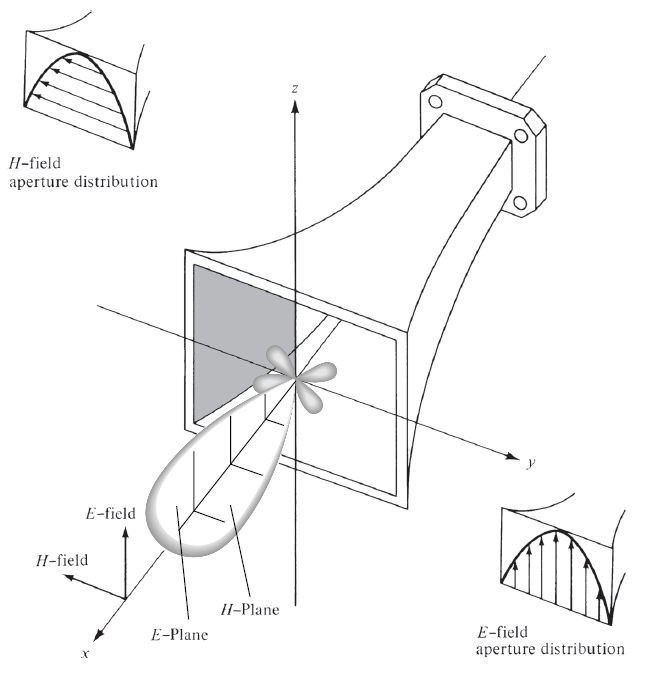
\includegraphics[scale=0.6]{chapters/ch3/assets/campoEH_piramidal}
\caption[Campos E e H de um diagrama de radiação de uma antena]{Campos E e H de um diagrama de radiação de uma antena}
\label{fig:campoEH_piramidal}
\end{figure}

\subsubsection*{Regiões de Campo}
De forma a identificar a estrutura do espaço circundante da antena, este é dividido em três regiões \parencite{Kraus1988}:
\begin{itemize}
\item Região reativa do campo próximo: Definida com a porção do espaço imediatamente em redor da antena, onde predomina o campo reativo;
\item Região do campo próximo (\textit{Região de Fresnel}): Definida como a região da antena entre a região reativa do campo próximo e a região de \textit{Fraunhofer} onde predomina o campo radiado e a sua orientação espacial depende da distância à antena;
\item Região do campo distante (\textit{Região de Fraunhofer}): Caraterizada pela região onde a distribuição angular do campo é maioritariamente independente da distância à antena.
\end{itemize}

Tipicamente, a forma diagrama de radiação é alterado consoante as regiões em que se encontra. Segundo a Figura \ref{fig:alt_tipicas_regioes} presente no artigo \cite{Y.RahmatL.WilliamsR.Yoccarino1995}, o diagrama é mais disperso e uniforme na região reativa do campo próximo. À medida em que a distância à antena aumenta, e que se entra nas regiões de \textit{Fresnel} e \textit{Fraunhofer} a forma do diagrama evidencia mais os seus lóbulos e fica mais regular. A separação entre as regiões reativa do campo próximo e região de \textit{Fresnel} e entre a região de \textit{Fresnel} e região de \textit{Fraunhofer} são definidas pelas expressões \ref{3.1} e \ref{3.2} respetivamente \parencite{Y.RahmatL.WilliamsR.Yoccarino1995}.

\begin{equation} \label{3.1}
R=\dfrac{2L^{2}}{\lambda}
\end{equation}

\begin{equation} \label{3.2}
R=0.62\sqrt{\dfrac{L^{3}}{\lambda}}
\end{equation}

\begin{figure}[h]
\centering
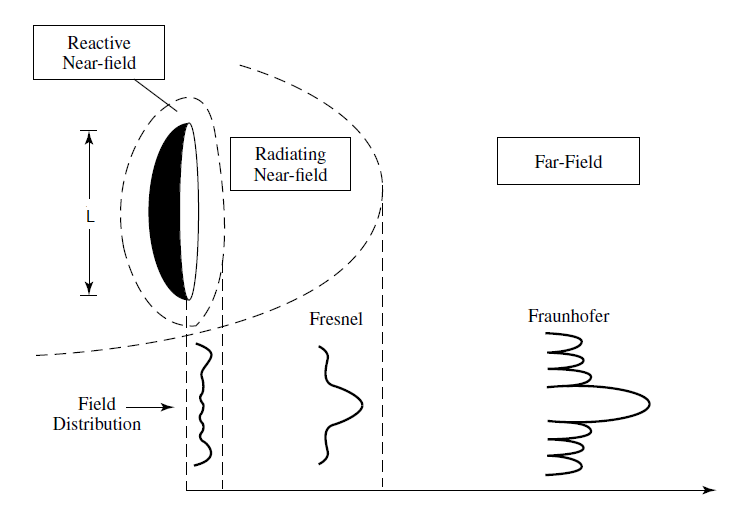
\includegraphics[scale=0.6]{chapters/ch3/assets/alt_tipicas_regioes}
\caption[Alterações típicas da forma do diagrama de radiação]{Alterações típicas do diagrama de radiação desde a reagião reativa do campo próximo à \textit{Região de Fraunhofer}. \parencite{Y.RahmatL.WilliamsR.Yoccarino1995}}
\label{fig:alt_tipicas_regioes}
\end{figure}


\subsection*{Densidade de Potência}

As ondas eletromagnéticas resultam da combinação de um campo magnético e de um campo elétrico que se propaga no espaço. A forma de representar a densidade direcional da quantidade de energia transferida de uma onda eletromagnética é através do vetor de \textit{Poynting}, o qual é definido, contabilizando variações temporais sinusoidais, na equação \ref{3.3}, expressa em \si{\watt\per\meter\squared}.

\begin{equation} \label{3.3}
W_{av}(x,y,z)=\dfrac{1}{2}Re[E\times H^{*}]
\end{equation}

Sendo que o vetor de \textit{Poynting} é uma densidade de potência, ao integrar a componente normal do mesmo, obtém-se na equação \ref{3.4} a potência média radiada pela antena $P_{rad}$ que atravessa uma superfície fechada S.

\begin{equation} \label{3.4}
P_{rad}=P_{av}=\oiint_S W_{rad}\cdot \,ds 
=\dfrac{1}{2} \oiint_S Re[E\times H^{*}]\cdot \,ds
\end{equation}

Como meio de comparação, define-se a potência radiada por um radiador isotrópico na expressão \ref{3.6}, com uma densidade de potência dada por,

\begin{equation} \label{3.5}
W_{0}=\hat{a}_{r}=\hat{a}_{r}\left( \dfrac{P_{rad}}{4\pi r^{2}}\right) 
\end{equation}

\begin{equation} \label{3.6}
P_{rad}=\oiint_S W_{rad}\cdot \,ds 
=\int_{0}^{2\pi}\int_{0}^{\pi}\left[ \hat{a}_{r}W_{0}(r)\right] \cdot \left[ \hat{a}_{r}r^{2}sin\theta \,d\theta \,d\phi \right] = 4\pi r^{2}W_{0}
\end{equation}
 
 
\subsection*{Diretividade}
A diretividade de uma antena é definida com a relação entre a intensidade de radiação numa determinada direção e a intensidade de radiação média em todos as direções. A intensidade média é igual ao quociente entre a potência total radiada pela antena e 4$\pi$ \parencite{IEEE1997}. Sendo que a intensidade de radiação $U$ é obtida pela multiplicação entre a densidade de radiação e o quadrado da distância, a diretividade $D$ de uma antena pode ser descrita pela expressão \ref{3.7}.

\begin{equation} \label{3.7}
D=\dfrac{U}{U_{0}}=\dfrac{4\pi U}{P_{rad}}
\end{equation}

No entanto, para antenas com componentes de polarização ortogonais podem-se definir diferentes diretividades parciais para cada polarização $\theta$ e $\phi$,

\begin{equation} \label{3.8}
D_{0}=D_{\theta}+D_{\phi}
\end{equation}

onde, 

\begin{equation} \label{3.8a}
D_{\theta}=\dfrac{4\pi U_{\theta}}{\left( P_{rad}\right)_{\theta}+\left( P_{rad}\right)_{\phi}}
\end{equation}

\begin{equation} \label{3.8b}
D_{\phi}=\dfrac{4\pi U_{\phi}}{\left( P_{rad}\right)_{\theta}+\left( P_{rad}\right)_{\phi}}
\end{equation}

sendo que o índice $\theta$ e $\phi$ representa a direção que contém as componentes do campo $\theta$ e $\phi$ respetivamente.

Para um radiador isotrópico, a diretividade toma o valor unitário, no entanto, em qualquer outro tipo de radiador, o valor da máxima diretividade irá ser sempre superior a ao valor unitário. Na equação \ref{3.7}, considerando o cálculo para a diretividade máxima, esta pode tomar valores inferiores a 1, o que não acontece na realidade. Com isto, uma expressão mais geral para a diretividade e para a diretividade máxima podem ser definidas na equação \ref{3.9a} e \ref{3.9b} respetivamente.

\begin{equation} \label{3.9a}
D\left( \theta ,\phi\right)=4\pi\dfrac{F\left( \theta ,\phi\right)}{\int^{2\pi}_{0}\int^{\pi}_{0}F\left( \theta ,\phi\right)sin\theta\,d\theta \,d\phi} 
\end{equation}

\begin{equation} \label{3.9b}
D_{0}=4\pi\dfrac{F\left( \theta ,\phi\right)\mid_{max}}{\int^{2\pi}_{0}\int^{\pi}_{0}F\left( \theta ,\phi\right)sin\theta\,d\theta \,d\phi} 
\end{equation}

onde $F\left( \theta ,\phi\right)$ é uma função dos componentes do campo elétrico numa região do campo distante, que, multiplicada por uma constante, resulta a intensidade de radiação.\par 
No entanto, a diretividade máxima também pode ser descrita em função do ângulo sólido de feixe $\Omega_{A}$,\footnote{O ângulo sólido {$\Omega$} é definido como um ângulo tridimensional no centro de uma esfera, que subentende na superfície da mesma uma área medida pelo quadrado do raio da esfera e toma valores adimensionais.}

\begin{equation} \label{3.13}
D_{0}=\dfrac{4\pi}{\dfrac{\left[ \int^{2\pi}_{0}\int^{\pi}_{0}F\left( \theta ,\phi\right) sin\theta\,d\theta \,d\phi\right]}{F\left( \theta ,\phi\right) \mid_{max}} }=\dfrac{4\pi}{\Omega_{A}} 
\end{equation}


\subsection*{Ganho}
A diretividade de uma antena é uma medida que descreve apenas a propriedades direcionais da antena. Por outro lado, o ganho, para além de estar relacionado com a diretividade, também tem em conta a eficiência da antena, discutida mais à frente neste capítulo.\par
O ganho de uma antena é um parâmetro fundamental na \textit{performance} da mesma. Este representa a eficiência em que a antena converte o sinal elétrico em ondas eletromagnéticas, que pode ser definido como ganho absoluto ou ganho relativo. O ganho absoluto de uma antena (definido na equação \ref{3.14}) representa a relação entre a intensidade de radiação radiada numa determinada direção e a intensidade de radiação que chega à antena, se a potência que chega à antena fosse radiada de forma isotrópica. No entanto, a antena isotrópica, como já foi falado neste capítulo, é um caso ideal e não corresponde à realidade. Com isto, utiliza-se o ganho relativo que relaciona a intensidade de radiação radiada de uma antena numa dada direção com a intensidade de radiação radiada a partir de outra antena na mesma direção, denominada antena de referência, quando ambas são alimentadas com a mesma potência de entrada.


\begin{equation} \label{3.14}
G\left( \theta ,\phi\right)=4\pi \dfrac{U\left( \theta ,\phi\right)}{P_{in}}
\end{equation}


Como falado mais à frente neste capítulo, a potência radiada $P_{rad}$ está relacionada com a potência de entrada $P_{in}$ da seguinte forma,

\begin{equation} \label{3.15}
P_{rad}=e_{cd}P_{in}
\end{equation}

sendo que $e_{cd}$ representa a eficiência de radiação da antena. \par 
A partir da equação \ref{3.15}, usando a \ref{3.14}, vem,

\begin{equation} \label{3.16}
G\left( \theta ,\phi\right)=e_{cd} \left[ 4\pi \dfrac{U\left( \theta ,\phi\right)}{P_{rad}}\right] 
\end{equation}

Que está relacionado com a diretividade (equação \ref{3.7}) da seguinte forma,

\begin{equation} \label{3.17}
G\left( \theta ,\phi\right)=e_{cd}D\left( \theta ,\phi\right)
\end{equation}

No entanto, a equação \ref{3.17} não contempla perdas quando o elemento da antena está conectado a um guia, o que provoca perdas indesejadas, através de reflexões. Isto pode ser solucionado com a introdução do termo $e_{r}$ que está relacionado com o coeficiente de reflexão,

\begin{equation} \label{3.18}
e_{r}=\left( 1-\vert\Gamma\vert^{2}\right) 
\end{equation}

Assim sendo, pode-se introduzir o conceito de ganho realizado $G_{re}$ que tem em conta as perdas por reflexão da antena.

\begin{equation} \label{3.19}
G_{re}\left( \theta ,\phi\right)=e_{r}G\left( \theta ,\phi\right)=\left( 1-\vert\Gamma\vert^{2}\right)G\left( \theta ,\phi\right)=e_{r}e_{cd}D\left( \theta ,\phi\right) 
\end{equation}

É de notar, que se a antena for adaptada ao guia, ou seja, se a impedância de entrada for igual à impedância característica ($\vert\Gamma\vert =0$), então, $G=G_{re}$.


\subsection*{Largura de Banda}
A largura de banda é uma gama de frequências, em redor de uma frequência central $f_{c}$, para a qual as caraterísticas da antena se mantêm com um valor aceitável relativamente aos valores obtidos para a frequência central. A largura de banda é, frequentemente, um dos parâmetros determinantes usados para dimensionar a antena.\par
Dependendo das necessidades de operação da antena que é utilizada, a largura de banda será limitada por certos fatores que são falados neste capítulo, como a impedância de entrada, ganho, forma do diagrama de radiação e polarização. Na prática, a largura de banda pode ser representada de duas formas,
\begin{itemize}
\item Antenas de banda larga, que apresentam a caraterística da frequência mais alta ser maior ou igual que o dobro da menor frequência. A largura de banda é representada pela razão entre estas frequências. Por exemplo, uma razão de 5:1 significa que a frequência mais alta é 4 vezes maior que a menor frequência.
\item Antenas de banda estreita, que são caraterizadas por apresentarem uma largura de banda muito menor que a frequência central. Neste caso, a largura de banda é expressa em percentagem. Por exemplo, uma percentagem de 10\% de banda larga significa que é aceitável que a diferença da menor frequência para a frequência central, e consequentemente a diferença da frequência central para a maior frequência tome um valor que seja metade dos 10\% para cada lado de $f_{c}$, ou seja, 5\% de $f_{c}$ para cada lado.
\end{itemize}


\subsection*{Polarização}
A polarização da antena é definida como a polarização da onda radiada pela mesma, que é definida como a direção do campo elétrico da onda radiada, que se nada for dito em contrário, se considera na direção da máxima radiação. No entanto, na prática, a polarização da onda radiada depende da direção de propagação, ou seja, podem existir diferentes polarizações em zonas diferentes do diagrama de radiação.\par
A polarização pode ser classificada como linear, circular ou elíptica. Uma polarização linear é caraterizada se o vetor que descreve o campo elétrico tiver sempre a mesma direção à medida que a onda se propaga. A polarização circular é caraterizada pelo vetor do campo elétrico que gira numa circunferência no plano $xy$ à medida que a onda se propaga, o que difere para a polarização elíptica, no facto das duas componentes do vetor campo elétrico girarem numa elipse no plano $xy$. Pode-se definir a polarização linear e circular como casos particulares da polarização elíptica (Figura \ref{fig:polari}), em que as componentes do campo elétrico são múltiplos de $\pi$ na polarização linear e têm módulos iguais e um desfasamento múltiplo impar de $\dfrac{\pi}{2}$ na polarização circular.\par 
%O campo instantâneo 
%Para as diferentes polarizações, a relação tempo-fase $\Delta\phi$ é diferente, \par 
%Polarização linear,

%\begin{equation} \label{3.23}
%\Delta\phi = \phi_{y}-\phi_{x}=n\pi, \quad n=0,1,2,3,...
%\end{equation}

\begin{figure}[h]
\centering
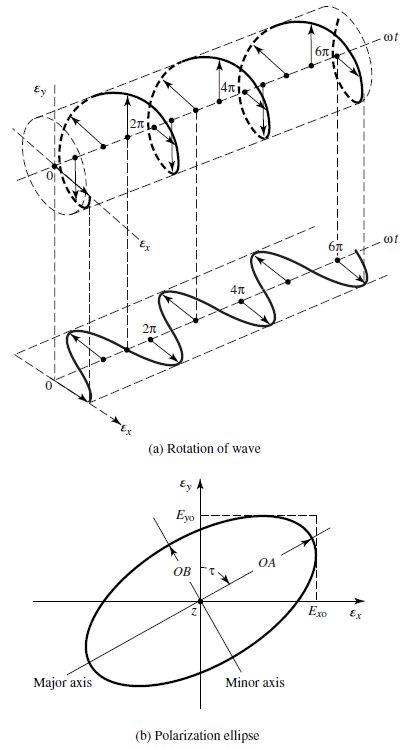
\includegraphics[scale=0.7]{chapters/ch3/assets/polari}
\caption[Alterações típicas da forma do diagrama de radiação]{Rotação de uma onda eletromagnética com polarização elíptica para $z=0$(Figura 2.23 \cite{Balanis2016}).}
\label{fig:polari}
\end{figure}

\subsubsection*{Perdas de Polarização}
As perdas de polarização ocorrem quando a polarização da antena recetora é diferente à da onda incidente. Devido a este fator, a potência extraída pela antena do sinal recebido não vai ser máxima.\par 
Assumindo que o campo elétrico da onda incidente pode ser escrito da seguinte forma,

\begin{equation} \label{3.23}
\mathbf{E_{i}}=\hat{\rho}_{w}E_{i}
\end{equation}

onde $\hat{\rho}_{w}$ é o vetor unitário da onda. Então, a polarização do campo elétrico da antena recetora pode ser escrito da seguinte forma,

\begin{equation} \label{3.24}
\mathbf{E_{a}}=\hat{\rho}_{a}E_{a}
\end{equation}

As perdas de polarização podem ser definidas pelo fator de perdas de polarização $PLF$, como na expressão \ref{3.25}.

\begin{equation} \label{3.25}
PLF=\vert\hat{\rho}_{w}\cdot \hat{\rho}_{a}\vert^{2}=\vert cos\psi_{p}\vert^{2}
\end{equation}

onde $\psi_{p}$ é o ângulo entre os dois vetores unitários.


%\subsection*{Impedância de Entrada}


\subsection*{Eficiência}
\subsubsection*{Eficiência da Antena}
A eficiência da antena $e_{0}$ descreve perdas nos terminais de entrada e dentro da estrutura da antena. A figura \ref{fig:perdas_antena} representa os terminais de referência da antena e as suas perdas: \begin{itemize}
\item Perdas por reflexão devido à não adaptação entre o guia e a antena
\item Perdas por condução e dielétrico
\end{itemize}

\begin{figure}[h]
\centering
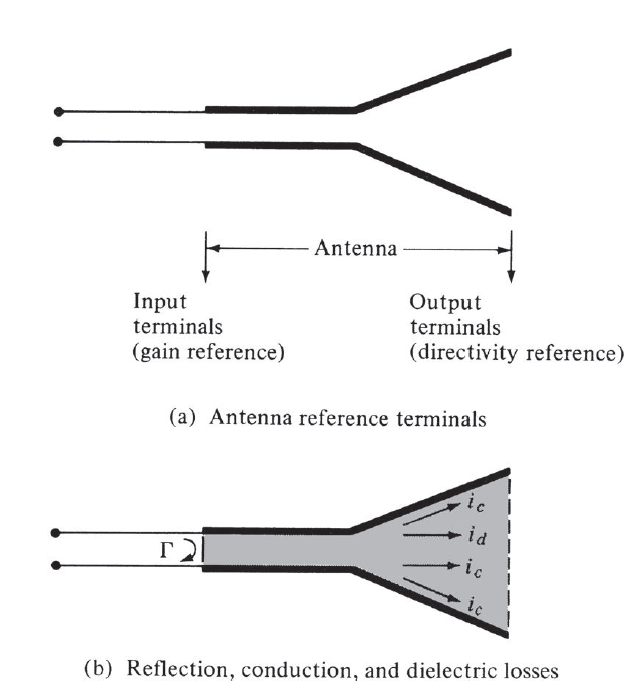
\includegraphics[scale=0.6]{chapters/ch3/assets/perdas_antena}
\caption[Terminais de referência e perdas na antena]{Terminais de referência e perdas na antena (Figura 2.22 do livro \cite{Balanis2016})}. 
\label{fig:perdas_antena}
\end{figure}

Ou seja, de modo geral, a eficiência pode ser escrita da seguinte forma,

\begin{equation} \label{3.20}
e_{0}=e_{r}e_{c}e_{d}
\end{equation}

onde \par 
$e_{0}$:"eficiência total" \par
$e_{r}$:"eficiência considerando perdas por reflexão $\left( 1-\vert\Gamma\vert^{2}\right)$"\par
$e_{c}$:"eficiência considerando perdas por condução"\par
$e_{d}$:"eficiência do dielétrico"\par
$\Gamma$:"coeficiente de reflexão nos terminais de entrada da antena"\par 
$\left[ \Gamma=(Z_{in}-Z_{0})/(Z_{in}+Z_{0})\right] $ com $ Z_{in}$: impedância de entrada e $Z_{0}$: impedância característica do guia.\par 
com a relação de onda estacionária ROE,
\begin{equation} \label{3.21}
ROE=\dfrac{1+\vert\Gamma\vert}{1-\vert\Gamma\vert}
\end{equation}

Por norma, $e_{c}$ e $e_{d}$ são muito difíceis de calcular, mas podem ser determinados experimentalmente. Com isto, é comum substituir-se $e_{c}e_{d}$ por $e_{cd}$ e representar-se a eficiência total $e_{0}$ por,

\begin{equation} \label{3.22}
e_{0}=e_{r}e_{cd}=e_{cd}\left( 1-\vert\Gamma\vert^{2}\right)
\end{equation}


%\subsubsection*{Eficiência do Feixe}
%Outro parâmetro para definir a qualidade de transmissão e receção é a eficiência de feixe $BE$.

%\subsection*{Máxima Diretividade e Máxima Área Efetiva}



\subsection*{Equação Radar} \label{subcap:eqradar}
A equação radar pode ser definida através do conhecimento da \gls{RCS} do alvo.\footnote{\gls{RCS} é uma representação da capacidade de um alvo de refletir um sinal radar na direção do recetor. Em regra a \gls{RCS} de um alvo é comparada com a força de um sinal refletido isotrópicamente de uma esfera perfeitamente lisa com uma área de secção transversal de $1m^{2}$ }\par 
A equação radar relaciona a potência recebida com a potência transmitida depois de ter sido refletida num alvo com uma \gls{RCS} $\sigma$

\begin{equation} \label{3.26}
\dfrac{P_{r}}{P_{t}}=e_{cdt}e_{cdr}\sigma \dfrac{D_{t}\left( \theta_{t},\phi_{t}\right)D_{r}\left( \theta_{r},\phi_{r}\right) }{4\pi}\left( \dfrac{\lambda}{4\pi R_{1}R_{2}}\right)^{2} 
\end{equation}

com \gls{RCS},

\begin{equation} \label{3.27}
\sigma =\lim_{R\to\infty}\left[ 4\pi R^{2}\dfrac{W_{s}}{W_{i}}\right] 
\end{equation}

onde \par 
$e_{cdr}$:"eficiência considerando perdas dielétrico e por condução no recetor" \par
$e_{cdt}$:"eficiência considerando perdas dielétrico e por condução no transmissor" \par
$R$:"distância do recetor ao alvo" \par
$W_{i}$:"Densidade de potência radiada" \par
$W_{s}$:"Densidade de potência recebida" \par

Se considerarmos perdas por reflexão vem,  

\begin{equation} \label{3.28}
\dfrac{P_{r}}{P_{t}}=e_{cdt}e_{cdr}\left( 1-\vert\Gamma_{t}\vert^{2}\right)\left( 1-\vert\Gamma_{r}\vert^{2}\right)\sigma \dfrac{D_{t}\left( \theta_{t},\phi_{t}\right)D_{r}\left( \theta_{r},\phi_{r}\right) }{4\pi}\times\left( \dfrac{\lambda}{4\pi R_{1}R_{2}}\right)^{2}\vert\hat{\rho}_{w}\cdot \hat{\rho}_{a}\vert^{2}
\end{equation}

onde \par 
$\Gamma_{r}$:"coeficiente de reflexão nos terminais de entrada da antena de receção" \par
$\Gamma_{t}$:"coeficiente de reflexão nos terminais de entrada da antena de transmissão" \par
$\hat{\rho}_{w}$:"vetor unitário de polarização nas ondas refletidas"\par
$\hat{\rho}_{r}$:"vetor unitário de polarização na antena de receção"\par

No entanto, se as antenas estiverem com polarização adaptada para a máxima radiação direcional e receção, a equação \ref{3.28} fica reduzida a,

\begin{equation} \label{3.29}
\dfrac{P_{r}}{P_{t}}=\sigma \dfrac{G_{0t}G_{0r}}{4\pi}\left( \dfrac{\lambda}{4\pi R_{1}R_{2}}\right)^{2} 
\end{equation}


%\subsection*{\textit{Radar Cross Section}}



%\subsection*{Temperatura da Antena}



\section{Simulação de uma Antena}
Conhecendo os parâmetros fundamentais de uma antena, descritos ao desenrolar deste capítulo, pode-se concluir que um dos principais problemas quando se juntam duas antenas como no caso desta atividade prática, é a interseção do diagrama de radiação, que se verifica no próximo subcapítulo com a figura \ref{fig:yagi}.\par
É possível obter maior diretividade numa antena e consequentemente menos interação entre os diagramas das mesma, no entanto alterar a configuração duma antena pode inserir lóbulos secundários entre outros problemas. Pode-se ainda melhorar a diretividade modificando a sua configuração elétrica a partir da geometria dos elementos radiantes.\par
Posto isto, considerando a experiência realizada, descrita no Capítulo \ref{chap:Chapter5}, é necessário compreender as propriedades da antena utilizada de modo a retirar conclusões confiáveis. Como falado, uma das propriedades mais importantes neste caso é o diagrama de radiação, que permite observar a diretividade da antena, visto que se o sinal direto é recebido nas duas antenas por estas serem pouco diretivas, torna a situação muito mais difícil, e os resultados muito menos fidedignos.

\subsection{Para Sinais DVB-T}
As antenas utilizadas para a experiência foram duas \textit{One for all Yagi-Uda} sv9354 para \gls{DVB-T} de $24 dB$.\par 
Para fazer a simulação do diagrama de radiação da antena utilizada, foi utilizada a \textit{toolbox antenna designer} do \textit{Matlab}, onde foram inseridas as caraterísticas da mesma obtendo como resultado a figura \ref{fig:yagi}. 

\begin{figure}[h]
\centering
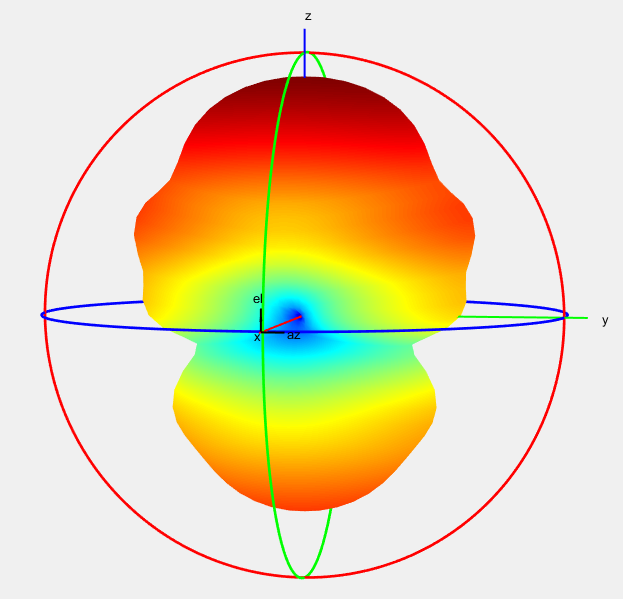
\includegraphics[scale=0.6]{chapters/ch3/assets/yagi}
\caption[Diagrama de radiação antena Yagi-Uda]{Diagrama de radiação da antena Yagi-Uda}
\label{fig:yagi}
\end{figure}

Com o diagrama de radiação da figura \ref{fig:yagi} que se encontra com a antena no sentido do eixo dos zz, ao duplicar e direcionar duas antenas para sentidos opostos ficamos com a configuração proposta para a experiência. Com isto, verificamos que há muita interação entre os lóbulos posteriores de cada antena, o que vai degradar muito o sinal. É então necessário ter este problema em consideração quando se tirar conclusões do trabalho.

% Chapter 4

\chapter{Processamento de Sinal} % Main chapter title
\label{chap:Chapter4} % For referencing the chapter elsewhere, use \ref{chap:Chapter4} 

%----------------------------------------------------------------------------------------

\section{Processamento de Sinal}
Como falado em \ref{contextualização}, o conceito do radar passivo é fazer uma \textit{cross-correlation} entre o sinal direto e o refletido. O problema está no facto de ser computacionalmente muito pesado fazer uma \textit{\gls{2D-CCF}}, sendo necessário a utilização de algoritmos mais eficientes para o cálculo da mesma.\par
O processamento de sinal num radar passivo pode ser, resumidamente, enumerado em oito pontos:
\begin{enumerate}
	\item Receção e reconstrução do sinal direto (\textit{reference signal}$s_{ref}$)
	\item Receção do \textit{surveillance signal} ($s_{r}$))
	\item \textit{Cross-correlation} do $s_{ref}$ e $s_{r}$
	\item Integração de produtos da correlação (FFT)
	\item Filtragem de \textit{clutter}
	\item Deteção de alvos e seguimento no domínio \textit{range/Doppler}
	\item Processamento no plano Cartesiano
	\item Seguimento no plano Cartesiano
\end{enumerate}

\subsubsection*{Equivalência entre um filtro adaptado e \textit{cross-correlation}}

Para \textit{Software Defined Radios}, a implementação de um filtro adaptado pode ser feita através do cálculo de uma \textit{cross-correlation} \parencite{Martorella}. Considerando $s_{0}(t)$ o sinal de saída do filtro adaptado e $h_{MF}(t)$ a resposta do filtro vem, 

\begin{equation} \label{4.1}
s_{0}\left( t\right) =s_{R}\left( t\right)\otimes h_{MF}\left( t\right) =\int s_{R}\left( \tau\right)s_{ref}^{\ast}\left(\tau -t\right)d\tau
\end{equation}

A equação \ref{4.1} mostra que usando um filtro adaptado obtemos um sinal de saída igual ao fazer uma \textit{cross-correlation} entre o $s_{R}$ e $s_{ref}$.\par 

Ao implementar uma \textit{cross-correlation} como mostrado em \ref{4.1}, não se toma em conta o desvio de \textit{Doppler}, visto que se faz a \textit{cross-correlation} apenas numa dimensão. Para se entrar com o desvio de \textit{Doppler} tem de se extender a \gls{2D-CCF},

\begin{equation} \label{4.2}
CCF\left( \tau,\nu\right) =\int s_{R}\left( \tau\right)s_{ref}^{\ast}\left(\tau -t\right)e^{-2\pi j\nu t}d\tau
\end{equation}

onde $\nu$ representa o desvio de \textit{Doppler} que é definido pela \textit{cross-correlation} entre o $s_{R}$ e $s_{ref}$ compensada com o \textit{Doppler shift}.\par
Como o \textit{delay-time} $\tau$ pode ser transformado em \textit{bistatic range}, a \gls{2D-CCF} pode ser representada num \textit{bistatic range-Doppler map}, através da equação \ref{4.3} que representa a \gls{2D-CCF} numéricamente visto que os sinais têm de ser digitalizados com uma certa frequência de amostragem.

\begin{equation} \label{4.3}
CCF\left(l,m\right) =\sum_{n=0}^{N-1} s_{R}\left( n\right)s_{ref}^{\ast}\left(n -l\right)e^{-2\pi j\dfrac{mn}{N}}
\end{equation}

onde $n$ representa o tempo, $l$ o \textit{delay-time}, $m$ o desvio de \textit{Doppler} e $N$ o número total de amostras que depende do \gls{CPI},

\begin{equation} \label{4.4}
N=\dfrac{CPI}{T_{s}}=CPI\cdot F_{s}
\end{equation}

\subsubsection*{Eficiência do cálculo da \gls{2D-CCF}}
De modo a ter um cálculo da \gls{2D-CCF} mais eficiente, há duas condições principais a referir:
\begin{itemize}
\item Cumprir com o teorema de \textit{Nyquist}, ou seja, garantir que a frequência de amostragem é superior ou igual à largura de banda ($F_{s}\geq B$); 
\item Ter um \gls{CPI} longo de forma a obter maior ganho de integração e consequentemente melhor relação sinal-ruído.
\end{itemize}
\par
No entanto, o cálculo de uma \gls{2D-CCF} é computacionalmente muito pesado, e isto pode ser demonstrado com um pequeno exemplo: Para uma largura de banda $B=10MHz$, um $CPI=1s$ e um número de \textit{range bins} e de \textit{doppler bins} igual a 1000 cada, implica um número de multiplicações muito elevado ($10000000\cdot 1\cdot 1000\cdot 1000=10000000000$ cálculos).\par
Para solucionar este problemas existem várias soluções numéricas, como \textit{Correlation FFT}, \textit{Direct FFT} e \textit{Batches Algorithm} \parencite{Martorella}.

\subsubsection*{\textit{Correlation FFT}}
A \textit{Correlation FFT} pode ser obtida através da equação \ref{4.3} mudando o exponencial de posição como representado na eq. \ref{4.5}, de modo a obter uma nova expressão que pode ser calculada como uma \textit{cross-correlation} a uma dimensão com uma compensação de \textit{Doppler}, ou seja, \textit{Doppler bin} ($m$), a \textit{\gls{CCF}} é a \textit{cross-correlation} entre o \textit{reference signal} $S_{ref}$ e o sinal direto com um \textit{Doppler shift}.

\begin{equation} \label{4.5}
CCF\left(l,m\right) =\sum_{n=0}^{N-1} s_{R}\left( n\right)e^{-2\pi j\dfrac{mn}{N}}s_{ref}^{\ast}\left(n -l\right)
\end{equation}

Substituindo $s_{R}\left( n\right)e^{-2\pi j\dfrac{mn}{N}}$ por $s_{R}(n,m)$ vem,

\begin{equation} \label{4.6}
CCF\left(l,m\right) =\sum_{n=0}^{N-1} s_{R}\left( n,m\right) s_{ref}^{\ast}\left(n -l\right)
\end{equation}

Com isto, e sabendo que as \textit{cross-correlations} são calculadas mais eficientemente no domínio de \textit{Fourier}, vem,

\begin{equation} \label{4.7}
CCF\left(l,m\right) = IDFT\left[ S_{R}\left( k,m\right)S_{ref}^{\ast}\left(k\right)\right] 
\end{equation}

com 

\begin{equation} \label{4.8}
S_{R}\left( k,m\right)  = DFT\left[ s_{R}\left( n,m\right) \right] 
\end{equation}

\begin{equation} \label{4.9}
S_{ref}\left( k\right)  = DFT\left[ s_{ref}\left( n\right) \right] 
\end{equation}

A \gls{DFT} da versão do sinal direto com \textit{Doppler shift} pode ser calculada apenas uma vez porque a variável $m$ apenas causa um desvio circular.
Com isto, pode-se tirar algumas conclusões \parencite{Martorella}:
\begin{itemize}
\item Apenas é necessário calcular a \textit{\gls{DFT}} de $s_{R}\left( n,m\right)$ uma vez para $m=0$, visto que para outros valores de $m$ podem ser obtidos com um desvio;
\item Em cada iteração, são calculadas N multiplicações complexas e uma \textit{\gls{IDFT}}.
\end{itemize}

Com isto, concluímos que quanto menos \textit{doppler bins} existirem em relação aos \textit{range bins}, mais eficiente será o cálculo. Este pode ser expressado através da seguinte função de complexidade:

\begin{equation} \label{4.10}
O_{CF}=2Nlog_{2}(N)+N_{f}[N+Nlog_{2}(N)]
\end{equation}

onde,
$N_{f}$: "Número de doppler bins"

\subsubsection*{\textit{Direct FFT}}
Por outro lado, a \textit{Direct FFT} é um método que, tal como a \textit{Correlation FFT} deriva da interpretação da equação \ref{4.3} mas, para cada \textit{time bin} $l$, a \textit{\gls{CCF}} é a \gls{DFT} do produto do sinal recebido com a versão conjugada com \textit{delay} do \textit{reference signal} $S_{ref}$.

\begin{equation} \label{4.11}
CCF\left(l,m\right) = DFT\left[ S_{R}\left( n\right)S_{ref}^{\ast}\left(n-l\right)\right] 
\end{equation}

Da interpretação da equação \ref{4.11} conclui-se que, para cada iteração, são calculadas N multiplicações complexas e u,a \gls{DFT}. A sua função de complexidade pode ser expressa através da expressão \ref{4.12}:


\begin{equation} \label{4.12}
O_{DF}=N_{\tau}[N+Nlog_{2}(N)]
\end{equation}

onde,
$N_{\tau}$: "Número de range bins"

Ao contrário da \textit{correlation FFT}, tal como se pode observar na função de complexidade, a eficiência deste método é dependente do $N_{\tau}$. Isto é, o número de iterações feitas neste método está diretamente relacionado com o número de \textit{range cells}: quanto maior for o número de \textit{range cells} do mapa \textit{range-Doppler}, menos eficiente é este método.\par

\begin{figure}[h]
\centering
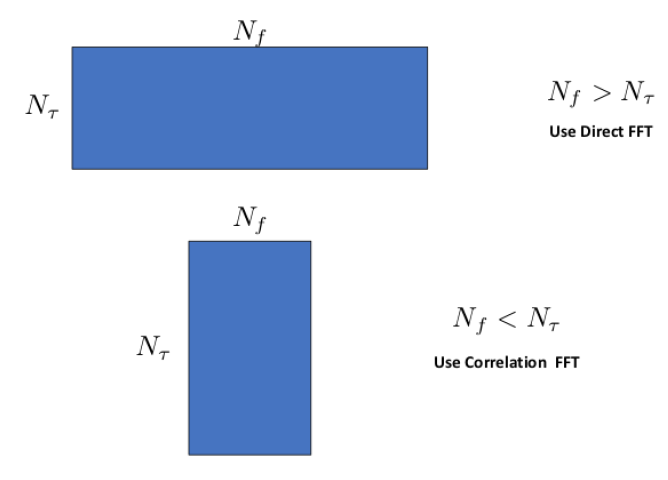
\includegraphics[scale=0.6]{chapters/ch4/assets/cfft_vs_dfft}
\caption[Correlation FFT vs Direct FFT]{\textit{Correlation FFT vs Direct FFT} (Figura 2.4 \cite{Martorella})}
\label{fig:cfft_vs_dfft}
\end{figure}

A figura \ref{fig:cfft_vs_dfft} representa de uma forma ilustrativa quando usar a \textit{Direct FFT} ou \textit{Correlation FFT} de acordo com a relação de \textit{Doppler cells} e \textit{range cells} no mapa de \textit{range-Doppler}. Se existirem mais \textit{Doppler cells} a \textit{Direct FFT} é mais eficiente, enquanto se o contrário se verificar, a \textit{Correlation FFT} torna-se mais eficiente.

\subsubsection*{\textit{Batches algorithm}}
Tanto os métodos \textit{direct FFT} e \textit{correlation FFT} são mais eficientes que fazer o cálculo da \gls{2D-CCF}, no entanto, dependem do número de \textit{range} ou \textit{doppler cells} e continuam a ser muito pesadas computacionalmente porque apenas otimizam o cálculo ao longo de uma dimensão.\par 
Apesar de não existir nenhum método perfeito que produza uma solução exata, um método denominado \textit{Batches algorithm} foi proposto e permite otimizar em duas dimensões com uma pequena perda de \textit{\gls{SNR}} reduzindo de forma considerável o peso computacional.\par
O \textit{Batches algorithm} consiste na subdivisão dos dois sinais recebidos, o sinal direto e o sinal refletido no alvo, em segmentos denominados \textit{batches}. Sendo $n_{B}$ o número de \textit{batches} e $N_{B}$ o comprimento do mesmo, com $N=n_{B}\cdot N_{B}$, a expressão da \gls{CCF} é representada pela equação \ref{4.13}.

\begin{equation} \label{4.13}
CCF\left( l,m\right)=\sum_{r=0}^{n_{B}-1}e^{\left( -j2\pi \dfrac{mrN_{B}}{N}\right)}\cdot \sum_{p=0}^{N_{B}-1}s_{R}\left( rN_{B}+p\right)s_{ref}^{\ast}\left( rN_{B}+p-l\right) e^{\left( -j2\pi \dfrac{mp}{N}\right)}   
\end{equation}

Este algoritmo assume que o efeito de \textit{Doppler} é negligenciado dentro de cada \textit{batch}, ou seja, só é calculado para o inicio de cada \textit{batch} $n_{B}$ e assim a equação \ref{4.13} é reduzida à equação \ref{4.14}.

\begin{equation} \label{4.14}
CCF\left( l,m\right)=\sum_{r=0}^{n_{B}-1}e^{\left( -j2\pi \dfrac{mrN_{B}}{N}\right)}\cdot \sum_{p=0}^{N_{B}-1}s_{R}\left( rN_{B}+p\right)s_{ref}^{\ast}\left( rN_{B}+p-l\right)
\end{equation}

A aproximação feita na eq. \ref{4.14} (frequência com que se calcula o desvio de \textit{Doppler}) pode ser representada por uma função \textit{step-wise} em vez de uma função linear (figura \ref{fig:phase_ap}).

\begin{figure}[h]
\centering
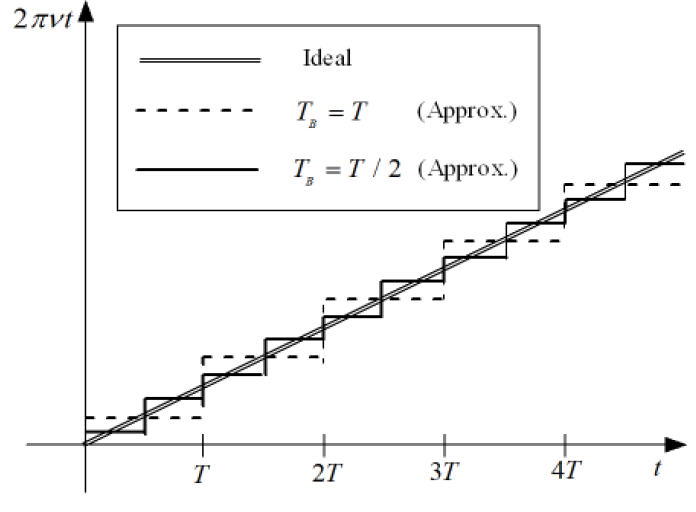
\includegraphics[scale=0.6]{chapters/ch4/assets/phase_ap}
\caption[Aproximação de fase]{Aproximação de fase da função de \textit{step} comparada com o ideal: função linear (Figura 2.6 \cite{Martorella})}
\label{fig:phase_ap}
\end{figure}

A equação \ref{4.14} pode ser interpretada de uma forma mais simples (eq. \ref{1.15})ao considerar o somatório do produto entre $s_{R}$ e $s_{R^{\ast}}$ como uma \gls{CCF} e a cada $n_{B}$ é calculado a \gls{DFT} ao longo de $r$.

\begin{equation} \label{4.15}
CCF\left( l,m\right)=\sum_{r=0}^{n_{B}-1}CCF\left( l,r\right) e^{\left( -j2\pi \dfrac{mrN_{B}}{N}\right)}=DFT\left[ CCF\left( l,r\right) \right] 
\end{equation}

Um dos fatores que influencia a eficiência do algoritmo é a escolha da duração dos \textit{batches}. Com isto, é simples concluir que para um determinado intervalo, ao escolher \textit{batches} com maior duração, vai existir um menor número de \textit{batches}, e consequentemente, a \gls{DFT} é calculada ao longo de um menor número de pontos o que vai levar a um menor tempo de processamento. No entanto, ao escolher \textit{batches} com maior duração, vai introduzir um erro maior na aproximação de fase e consequentemente mais perdas em \gls{SNR}.\par
Contudo, \textit{batches} com menor duração implicam o contrário, ou seja, maior número de batches, maior tempo de processamento e menos perdas em \gls{SNR}. \par 
Foi desenvolvido um estudo de grande interesse \parencite{Petri2012} que analisa extensivamente a utilização do \textit{batches algorithm} em que foram recolhidos dados com um radar passivo da \gls{CNIT}. Os resultados da análise da duração dos \textit{batches} com o tempo de processamento e perdas \gls{SNR} encontram-se representados na tabela e figura \ref{fig:bat_snr} respetivamente.\par 

\begin{table}[h]
\centering
\begin{tabular}{@{}ccccc@{}}
\toprule
Comprimento do batch & Tempo de processamento  \\ \midrule
31.28 $\mu s$        & 4.93 $s$                \\
218.76 $\mu s$       & 0.92 $s$                \\
333.29 $\mu s$       & 0.71 $s$                \\ 
924 $\mu s$          & 0.59 $s$                \\ \bottomrule
\label{tab:Tempo de processamento}
\end{tabular}
\caption[\textit{Batches algorithm} - tempo de processamento]{\textit{Batches algorithm} - Análise do tempo de processamento devido ao comprimento dos \textit{batches} (Tabela 2.1 \cite{Martorella})}
\end{table}

\begin{figure}[h]
\centering
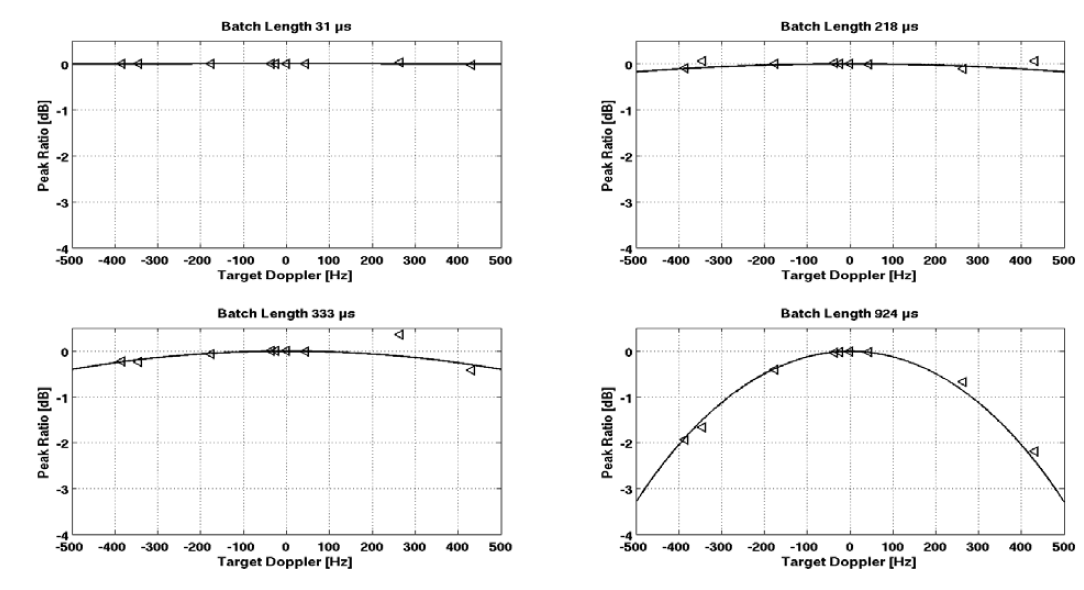
\includegraphics[scale=0.5]{chapters/ch4/assets/bat_snr}
\caption[Perdas SNR]{\textit{Batches algorithm} - Análise perdas \gls{SNR} devido ao comprimento dos \textit{batches}(Figura 2.8 \cite{Martorella})}
\label{fig:bat_snr}
\end{figure}



\subsection{Cancelamento de \textit{clutter}}
No funcionamento do radar passivo, um dos sinais que se quer ter conhecimento é o sinal direto, que é o sinal que é transmitido diretamente do iluminador de oportunidade para o recetor, como representado na figura \ref{fig:esquema_pcl}. Este sinal é submetido a uma atenuação  %de $1/C^{2}$ \parencite{Griffiths2017}, onde $C$ é a \textit{baseline} representada na figura \ref{fig:geom}.
pequena relativamente ao sinal refletido, isto porque a \textit{baseline} $C$ representada na figura \ref{fig:geom} é sempre menor que o \textit{bistatic range}. Logo, o sinal direto pode ser muito mais forte comparado com os ecos dos alvos, o que dificulta a deteção de alvos.\par 

\begin{figure}[h]
\centering
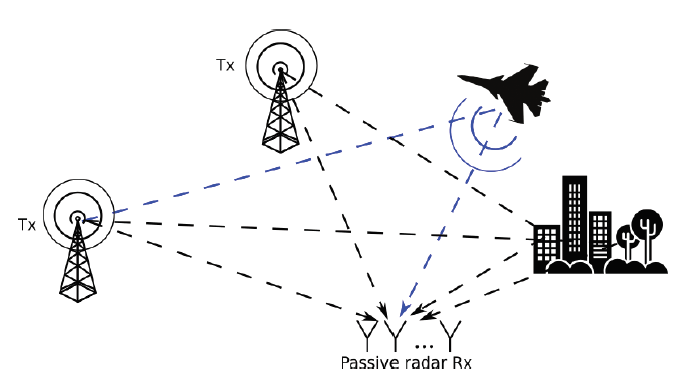
\includegraphics[scale=0.6]{chapters/ch4/assets/clutter}
\caption[Cenário PCL - Clutter]{Cenário PCL - Clutter (Figura 1 \cite{Peto2018})}
\label{fig:clutter}
\end{figure}


Por mais que se tente fisicamente não receber o sinal direto na antena de \textit{surveillance}, este e todas as suas cópias atrasadas no tempo devido a reflexões em objetos e terreno não desejadas (\textit{clutter} representado na figura \ref{fig:clutter}) são mais fortes que o sinal refletido no alvo. É possível haver reflexões em edifícios ou algo perto da antena de \textit{surveillance} que possam ser confundidas com o sinal que pretendemos obter, o que pode complicar o cancelamento de todas as réplicas do sinal indesejadas. É de notar, que no caso dos radar \textit{\gls{PCL}}, ou seja, radares passivos, estamos perante uma geometria bistática e isto leva a que o nível de \textit{clutter} na zona da \textit{baseline} possa ser muito forte e ser notável em algumas \textit{range cells}. Este efeito em junção com o sinal direto que possa ser captado na antena de \textit{surveillance} podem dificultar a deteção de alvos.\par 
O sinal recebido pode ser interpretado de uma forma mais realista como na equação \ref{4.16} para facilitar os processos de cancelamento de \textit{clutter} e identificação das diferentes componentes do sinal.


\begin{equation} \label{4.16}
S_{R}=A_{R}s_{T}\left( t\right)+\sum_{m=1}^{N_{T}}a_{m}s_{T}\left( t-\tau_{T_{m}}\right)e^{\left( 2\pi j f_{D_{m}}t\right)}+\sum_{i=1}^{N_{s}}b_{i}s_{T}\left( t-\tau_{c_{i}}\right)+n\left( t\right)    
\end{equation}

Onde o primeiro termo representa a componente do sinal direto, o segundo termo representa o sinal refletido no alvo, o terceiro termo representa o \textit{clutter} e por fim, o quarto termo representa a componente de ruído.\par

Os aspetos mais importantes na \textit{performance} do cancelamento de \textit{clutter} são a capacidade de operação em tempo real e a eficiência do algoritmo representada no mapa \textit{range-Doppler}. De modo geral, a filtragem, ou cancelamento de \textit{clutter} é feita em dois domínios diferentes: Técnicas de supressão no domínio do espaço para lidar com interferências de alta potência e algoritmos de filtragem de \textit{clutter} no domínio do tempo. Tem sido investigado a aplicação de vários métodos e o artigo \cite{Peto2018} resume a aplicabilidade e comparação de resultados obtidos na utilização dos mesmos tanto como uma explicação sucinta na sua execução.\par 

Existem várias técnicas de cancelamento de \textit{clutter} utilizadas em radares passivos. Os algoritmos de filtragem no domínio do tempo utilizam o \textit{reference signal} de modo a cancelar as réplicas do sinal com um desvio no tempo e de \textit{Doppler} no canal de \textit{surveillance}. Entre estes podemos salientar a aplicação das técnicas de filtragem de \textit{Wiener} com \textit{sample matrix inversion}, \gls{ECA}, \gls{ECA-B}, \gls{ECA-S} \gls{SCA}, \gls{LMS}, \gls{NLMS} e \gls{RLS}.\par

Como jeito de conclusão deste tópico, as figuras \ref{fig:doppler_cancelationtec} e \ref{fig:comp_cost}, retiradas do estudo \cite{Petri2012}  representam a \textit{performance} dos 
vários algoritmos nos dois aspetos mais relevantes, respetivamente no mapa de \textit{range-Doppler} que permite a observação da distorção e resolução do algoritmo e do aumento de \gls{SINR} em relação ao custo computacional  medido em \gls{FLOPS}.


\begin{figure}[h]
\centering
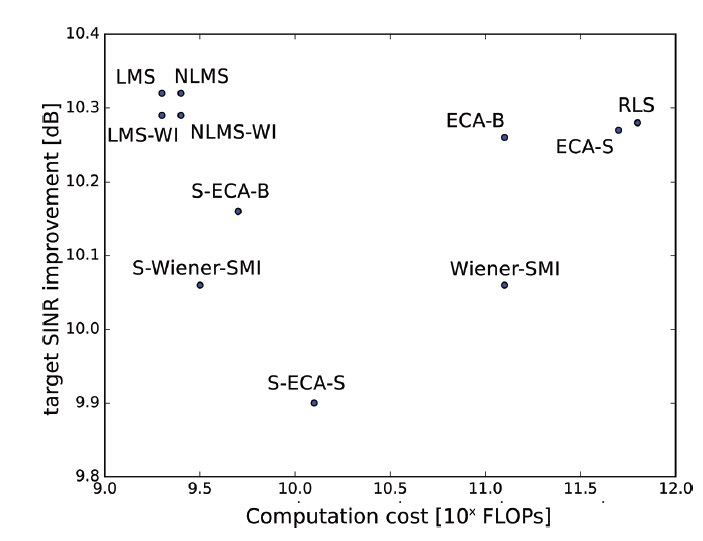
\includegraphics[scale=0.5]{chapters/ch4/assets/comp_cost}
\caption[Mapa da performance dos algoritmos]{Mapa da \textit{performance} dos algoritmos de acordo com o aumento de \gls{SINR} e \textit{computation cost} em \gls{FLOPS} (Figura 16 \cite{Peto2018})}
\label{fig:comp_cost}
\end{figure}

\begin{figure}[h]
\centering
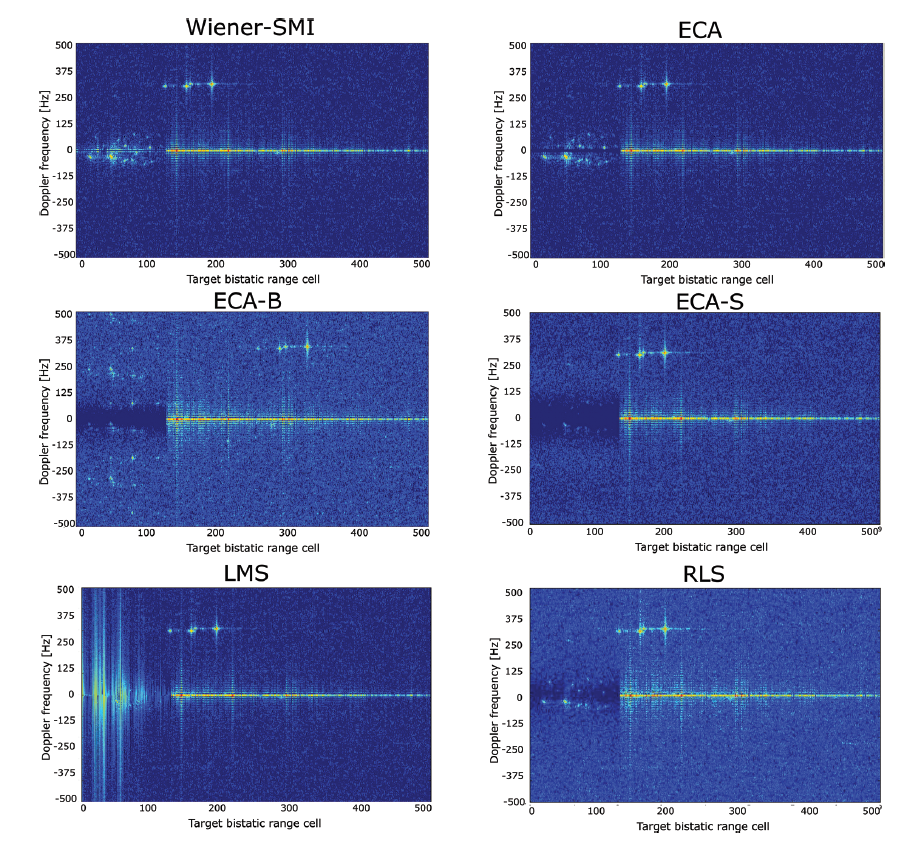
\includegraphics[scale=0.5]{chapters/ch4/assets/doppler_cancelationtec}
\caption[Mapas de range-Doppler dos diferentes algoritmos utilizados]{Mapas de \textit{range-Doppler} dos diferentes algoritmos utilizados (Figura 14 \cite{Peto2018})}
\label{fig:doppler_cancelationtec}
\end{figure}


Destes resultados obtidos, é de realçar o algoritmo \gls{ECA-S} que obteve a melhor \textit{performance} ao custo de um grande \textit{computation cost}. Contudo, pode-se observar os algoritmos do tipo \gls{LMS} e \gls{NLMS}, que apesar de terem um bom aumento de \gls{SINR} com pouco custo computacional, apresentam, como observável na figura \ref{fig:doppler_cancelationtec}, uma grande distorção no mapa \textit{range-Doppler}. Também é de notar, que na figura \ref{fig:comp_cost}, o aumento de \gls{SINR} é pouco relativamente ao custo computacional, isto porque o referencial não está normalizado, ou seja, a janela do eixo das ordenadas toma valores entre $9.8$ e $10.4 dB$ enquanto a janela do eixo das abcissas toma valores entre $10^{9}$ e $10^{12} FLOPS$.


\subsection{Reconstrução e equalização do sinal direto}
Uma das principais diferenças do radar passivo para o radar ativo é que no último o \textit{reference signal} é conhecido visto que é transmitido pelo próprio radar. No caso do radar passivo, a utilização de iluminadores de oportunidade tem como consequências o não conhecimento do sinal direto, visto que para além de receber o mesmo, recebemos as suas réplicas atrasadas no tempo e em \textit{Doppler} e ainda ruído.\par 
De forma a melhorar o sinal direto em quando este é digital, neste subcapítulo vão ser discutidos dois métodos diferentes para a remoção de \textit{multipath} e remoção de picos espúrios formados na função de ambiguidade.

\subsubsection*{Reconstrução do sinal direto} \label{Reconstrução do sinal direto}
Alguns sinais digitais transmitidos, como \gls{DVB-T} em específico, permitem a reconstrução do sinal direto através da desmodulação e re-modulação do sinal direto recebido. Por forma a reconstruir o sinal direto, no caso da \gls{DVB-T}, é importante conhecer o comprimento do símbolo exprimido em amostras, isto porque se a frequência de amostragem do transmissor e do recetor for igual, o comprimento do sinal em amostras é inteiro e a sua receção consiste em meter o sinal no domínio da frequência, usando uma \gls{FFT}. Se este não for o caso, ou seja, que a frequência de amostragem do recetor não seja a definida pelo \textit{standard} \gls{DVB-T}, o comprimento do símbolo não vai ser um número inteiro e a constelação do sinal recebido vai ficar distorcida visto que os pontos depois de usar a \gls{FFT} não vão corresponder às posições de cada subportadora. As soluções para este problema podiam passar por fazer uma nova amostragem do sinal por interpolação, mas isso ia introduzir grandes distorções. Existem várias soluções para este problema, como a utilização de outras transformadas, como a \gls{CZT}.\par 
O próximo passo na receção do sinal \gls{DVB-T} é descodificar os símbolos \gls{OFDM}. Este processo passa por o cálculo inverso no espetro do sinal que foi realizado no transmissor, ou seja, se foi usado uma \gls{FFT} no transmissor, para descodfidicar os símbolos \gls{OFDM} usa-se uma \gls{IFFT}. É de notar que, como falado no parágrafo anterior, se a frequência de amostragem for diferente no transmissor e recetor, a \gls{FFT} que é o mais comum, não pode ser usada. Ao invés, usa-se um método baseado na \gls{CZT}, que não é abordado nesta dissertação, mas pode ser compreendido, tal como todo o processo de reconstrução do sinal direto para radares passivos no estudo \cite{Baczyk2011}.\par 
De seguida, tem-se uma constelação do sinal direto reconstruido como na figura \ref{fig:64QAM} e o próximo passo é a reprodução do sinal no domínio do tempo sem o efeito de \textit{multipath}.

\begin{figure}[h]
\centering
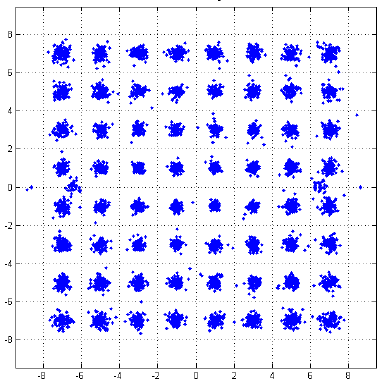
\includegraphics[scale=0.7]{chapters/ch4/assets/64QAM}
\caption[Constelação 64QAM]{Constelação 64QAM (Figura 3.4 \cite{Martorella})}
\label{fig:64QAM}
\end{figure}


\subsubsection*{Equalização do sinal direto}
Em adição à remoção do efeito \textit{multipath} com a reconstrução do sinal direto, é possível equalizar o sinal de forma a remover picos espúrios formados na função de ambiguidade como representados na figura \ref{fig:ACF} relativamente a sinais \gls{DVB-T}.

\begin{figure}[h]
\centering
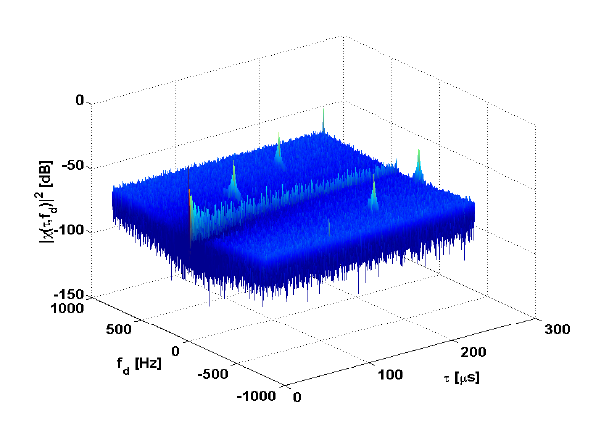
\includegraphics[scale=0.7]{chapters/ch4/assets/ACF}
\caption[Função de ambiguidade - Sinal DVB-T]{Função de ambiguidade - Sinal DVB-T - Presença de picos espúrios (Figura 3.5 \cite{Martorella})}
\label{fig:ACF}
\end{figure}

Um algoritmo eficiente para remover estes picos espúrios passa por estimar tanto para o sinal direto $S_{ref}$ como para um sinal, neste caso \gls{DVB-T}, gerado localmente uma função de \textit{\gls{PSD}} e, equalizar através de uma função de filtragem $H$ que posteriormente, é multiplicada com a transformada do sinal direto $S_{ref}$. De seguida é aplicada a \gls{IFFT} de forma a gerar um sinal direto mais limpo. Um esquema de blocos do algoritmo está representado na figura \ref{fig:equal}.

\begin{figure}[h]
\centering
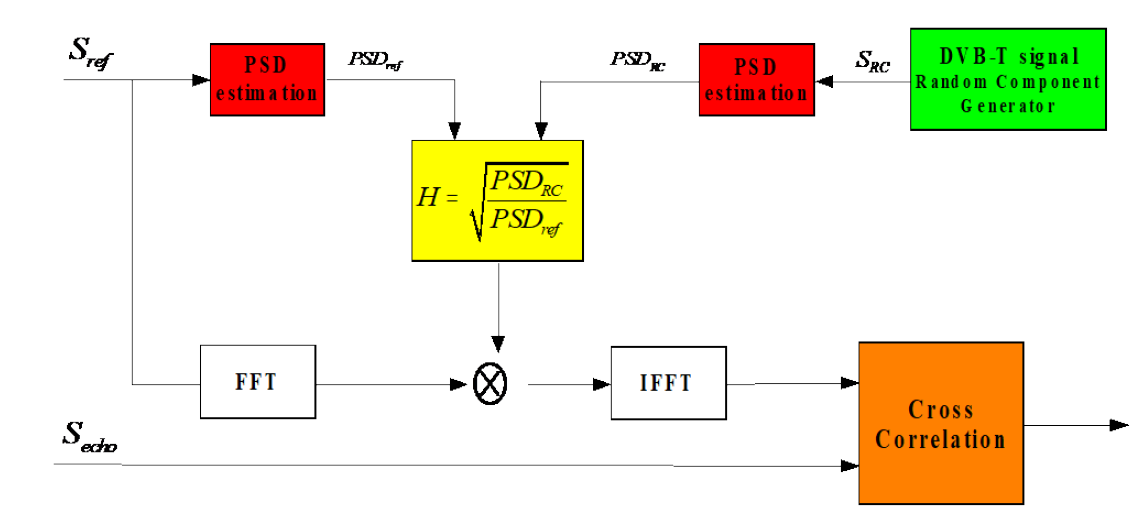
\includegraphics[scale=0.5]{chapters/ch4/assets/equal}
\caption[Diagrama de blocos - Algoritmo de equalização]{Diagrama de blocos - Algoritmo de equalização(Figura 3.6 \cite{Martorella})}
\label{fig:equal}
\end{figure}



\section{Simulação}

\subsection{Função de Ambiguidade}
Uma ferramenta que permite analisar as propriedades do sinal utilizado como iluminador de oportunidade é a função de ambiguidade. Esta função é bidimensional no \textit{time-delay} e em \textit{Doppler}, que representa a distorção devido ao filtro adaptado do recetor, falado no inicio deste capítulo e às propriedades do sinal.\par 
Para um sinal $s(t)$, a sua função de ambiguidade é obtida pela equação \ref{4.17}.

\begin{equation} \label{4.17}
\chi\left( \tau,f\right) =\int s\left( t\right)s^{\ast}\left( t-\tau\right)e^{2\pi jft}dt
\end{equation}

, ou seja, a auto-correlação do sinal recebido.

Utilizando o \textit{matlab} e as ferramentas que este dispõe, é possível calcular funções de ambiguidade de diversos sinais, tendo como um exemplo a figura \ref{fig:ambfun_fmdef} que é resultado do código em anexo \ref{Annex1} apresentado pelo matlab para fazer funções de ambiguidade consoante as caraterísticas do sinal.
\begin{figure}[h]
\centering
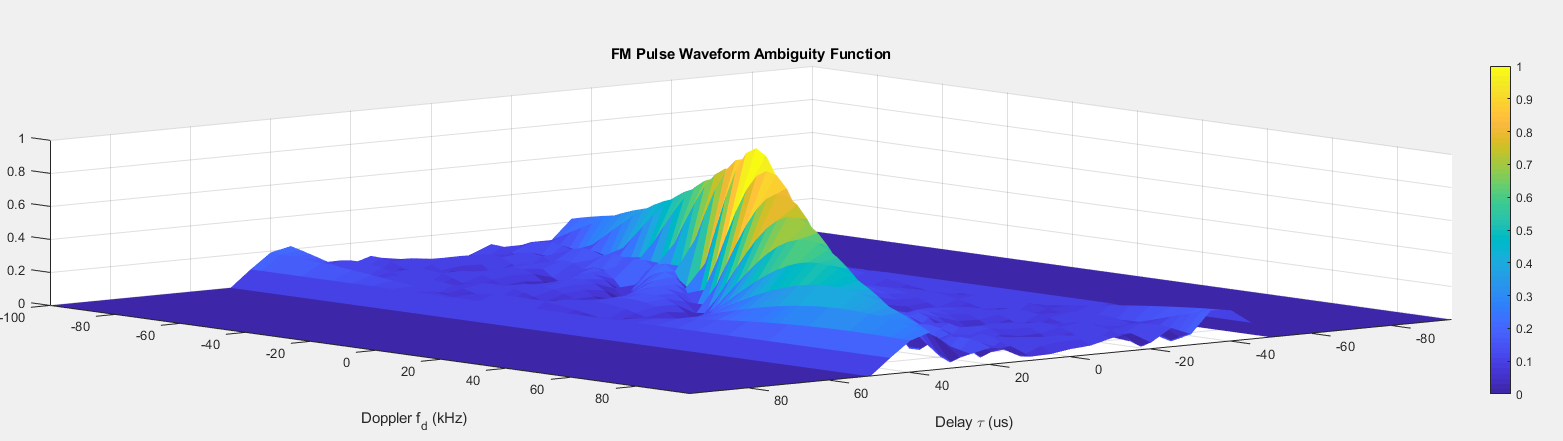
\includegraphics[scale=0.4]{chapters/ch4/assets/ambfun_fmdef}
\caption[Função de ambiguidade para um pulso FM]{Função de ambiguidade para um pulso FM}
\label{fig:ambfun_fmdef}
\end{figure}


\subsubsection{Sinais FM}
Um dos fatores que influencia a performance do sistema é a largura de banda, o que no caso de sinais \gls{FM} é dependente do tipo de música que é transmitido.\par
A figura \ref{fig:ambfun2} é retirada de uma estação a transmitir notícias que corresponde aos gráficos de cima e a transmitir música pop, representado no gráfico de baixo. As principais conclusões que se podem retirar da análise da função de ambiguidade de ambas é que quando é transmitida música, especialmente estilos de músicas como \textit{hard rock}, a largura de banda do sinal transmitido aumenta o que provoca uma função mais estreita e com menor intensidade em redor dos planos de zero \textit{Doppler} e zero \textit{delay}. Consequentemente, este tipo de transmissões permitem uma melhor deteção não só em alcance, como em \textit{Doppler}.

\begin{figure}[h]
\centering
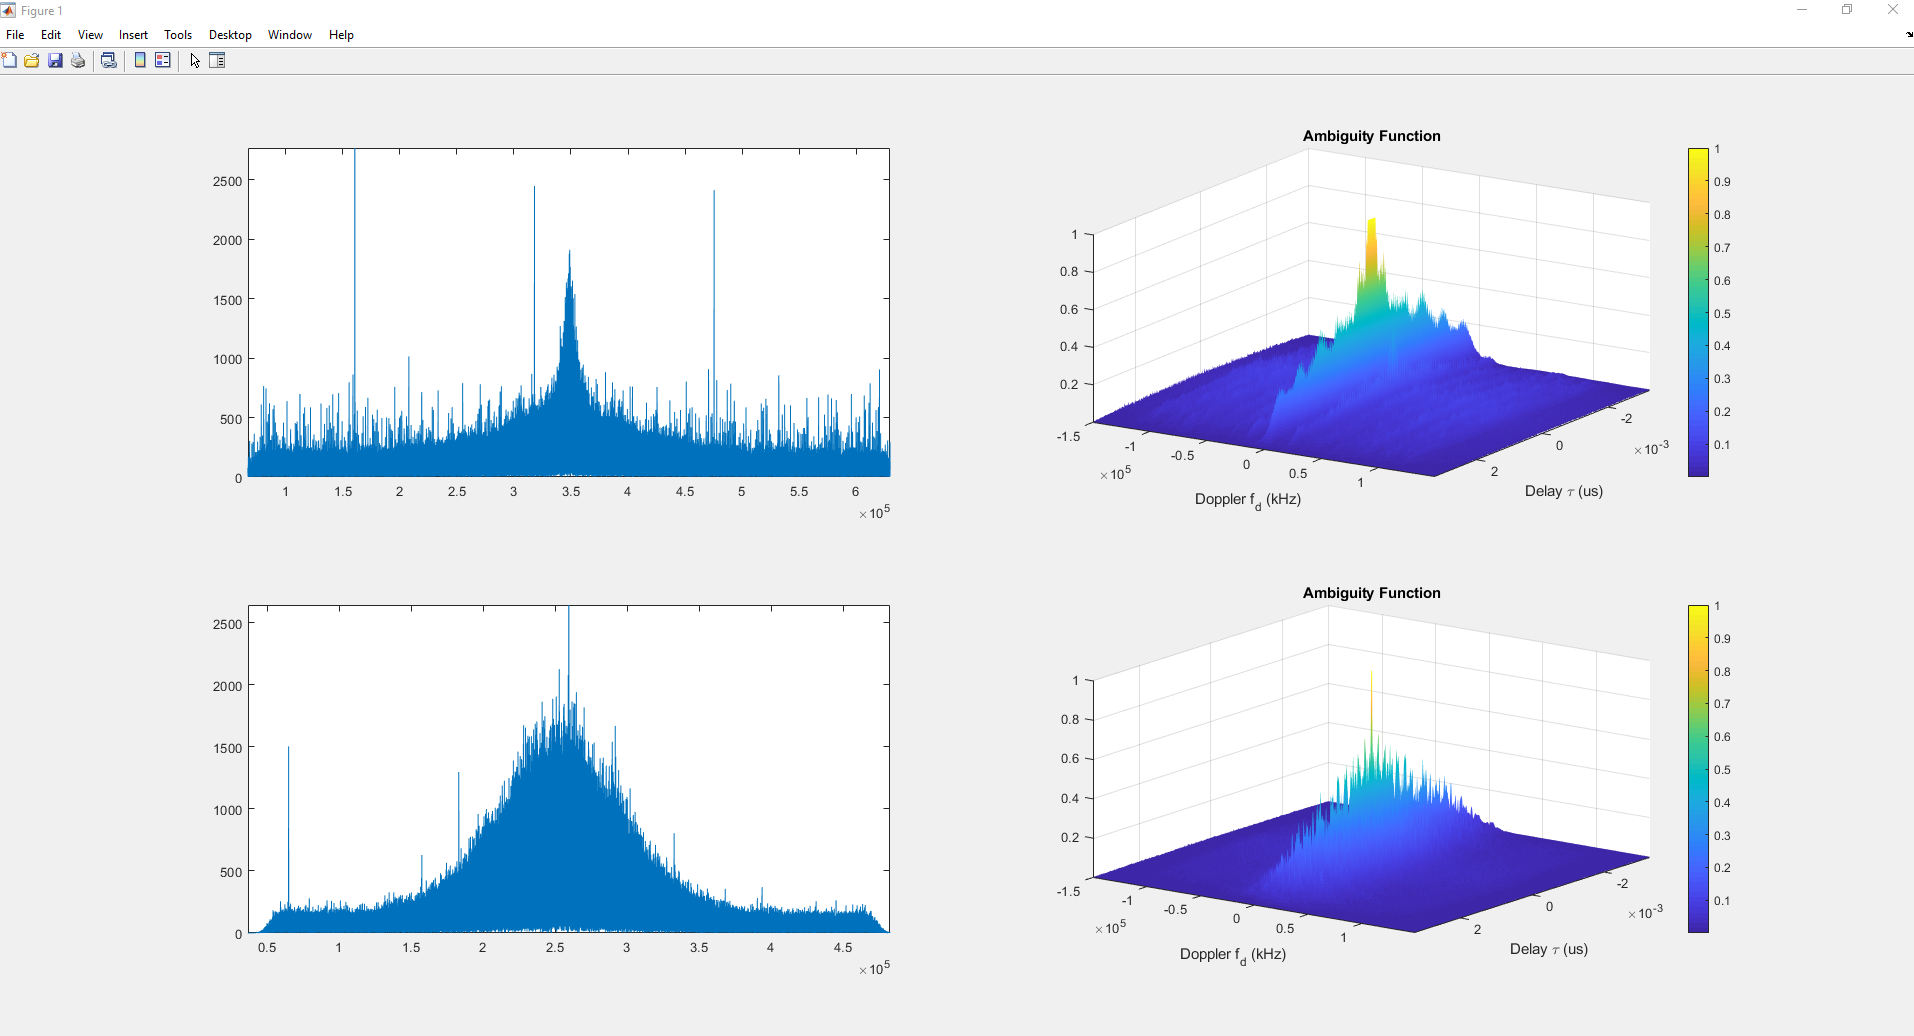
\includegraphics[scale=0.3]{chapters/ch4/assets/ambfun2}
\caption[Função de ambiguidade para uma estação FM]{Função de ambiguidade para um pulso FM retirada de uma estação a dar notícias e música pop}
\label{fig:ambfun2}
\end{figure}
 


\subsubsection{Sinais DVB-T}
Para obter as funções de ambiguidade dos sinais \gls{DVB-T} foi utilizado o LimeSDR com duas antenas de $24 dB$, como descrito no Capítulo \ref{chap:Chapter6}. É de notar que que a antena utilizada no lado direito tem um ganho relativamente superior, o que se deve às fichas que foram cravadas, mas que não tem muito impacto na função de ambiguidade. Dito isto, é mais adequado utilizar este canal para o sinal refletido e o com menor ganho para o sinal direto.\par 

\begin{figure}[h]
\centering
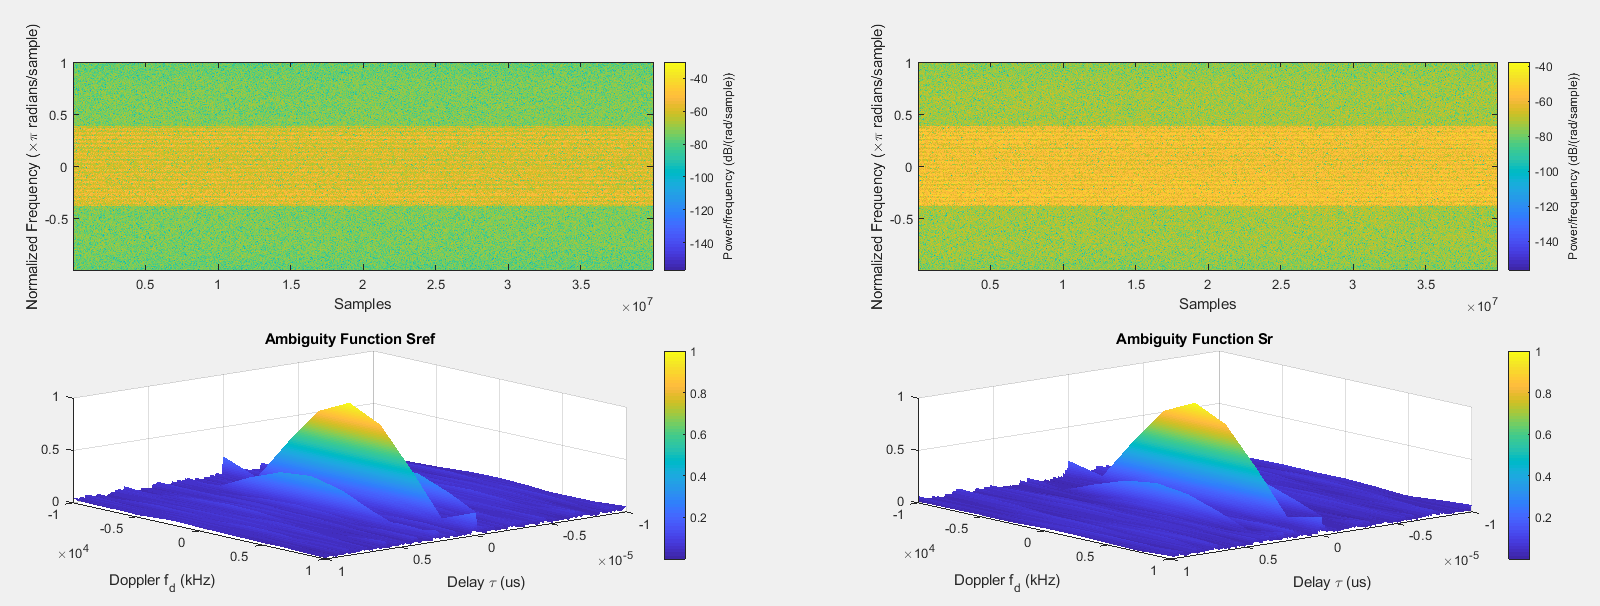
\includegraphics[scale=0.35]{chapters/ch4/assets/dvbt}
\caption[Função de ambiguidade para dois sinais DVB-T]{Função de ambiguidade para dois sinais DVB-T}
\label{fig:dvbt}
\end{figure}
 
Através da equação \ref{4.18}, na frequência $f_{0}=602 MHz$ que é utilizada nesta zona para \gls{DVB-T}, com $c=3x10^{8}m/s$, obtém-se um valor de de variação de frequência de $100Hz$ para $50m/s=180km/h$, ou seja, para uma distância ao alvo com valores inferiores a $15m$, segundo a equação \ref{4.19} para um \textit{delay} de $1\times 10^{-7}$, é muito difícil a deteção da velocidade do alvo.

\begin{equation} \label{4.18}
\Delta f=\dfrac{\Delta v}{c}f_{0}
\end{equation}

\begin{equation} \label{4.19}
Range=\dfrac{c\times delay}{2}
\end{equation}



@% Chapter 5

\chapter{Aplicação} % Main chapter title
\label{chap:Chapter5} % For referencing the chapter elsewhere, use \ref{chap:Chapter5} 

%----------------------------------------------------------------------------------------
\section{Sistema Desenvolvido}
O objetivo principal da parte prática da dissertação é não só recolher sinais e criar a sua função de ambiguidade, mas principalmente detetar um objeto estático e em movimento.
Para realizar estas tarefas foi utilizado um transmissor e recetor LimeSDR USB. As suas principais caraterísticas estão apresentadas na seguinte tabela e a sua documentação em \url{https://wiki.myriadrf.org/LimeSDR-USB}.\par

\begin{table}[h]
\centering
\begin{tabular}{@{}ccccc@{}}
\toprule
Caraterística       			 & Descrição                      \\ \midrule
\textit{RF Transreceiver}        & LMS7002M                       \\
\textit{Oscillator}    			 & Rakon RPT7050A @30.72$MHz$    \\
Banda de frequência              & 100$kHz$ - 3.8$GHz$            \\ 
Largura de banda máxima          & 61.44$MHz$                     \\ \bottomrule
\label{tab:limesdr}
\end{tabular}
\caption[Caraterísticas do LimeSDR USB]{Caraterísticas do LimeSDR USB}
\end{table}

Por forma a reduzir o ruído a alimentação é feita através dum \textit{power bank} de 20000$mAh$. Isto é conseguido com um cabo em "Y" que vem com o LimeSDR, que separa a entrada de dados da alimentação do equipamento.\par 
As duas antenas utilizada tanto para o canal de receção do sinal direto como do sinal refletido são antenas \textit{One for all} \textit{Yagi} de exterior para televisão, com $24dB$.\par 
Para a ligação entre o \textit{LimeSDR} e as antenas foram utilizados cabos coaxiais RG-58 com $1m$ de comprimento onde foram cravadas fichas SMA, como representado na figura \ref{fig:limec}.\par 
O repositório que contém as drivers que permitem trabalhar com o LimeSDR a partir do MATLAB foram desenvolvidos inicialmente e disponibilizado no link \url{https://github.com/jocover/Simulink-MATLAB-LimeSDR} em Agosto de 2017 pelo autor Jocover, posteriormente adaptado e atualizado em Dezembro de 2019 pelo autor Damir Rakhimov para a versão do LimeSuite 19.04 e pode ser acedido no \textit{github} do mesmo, \url{https://github.com/RakhDamir/LimeSDR-Matlab}. Todos os passos de instalação e configuração do sistema encontram-se disponibilizados no seu \textit{github}.

\begin{figure}[h]
\centering
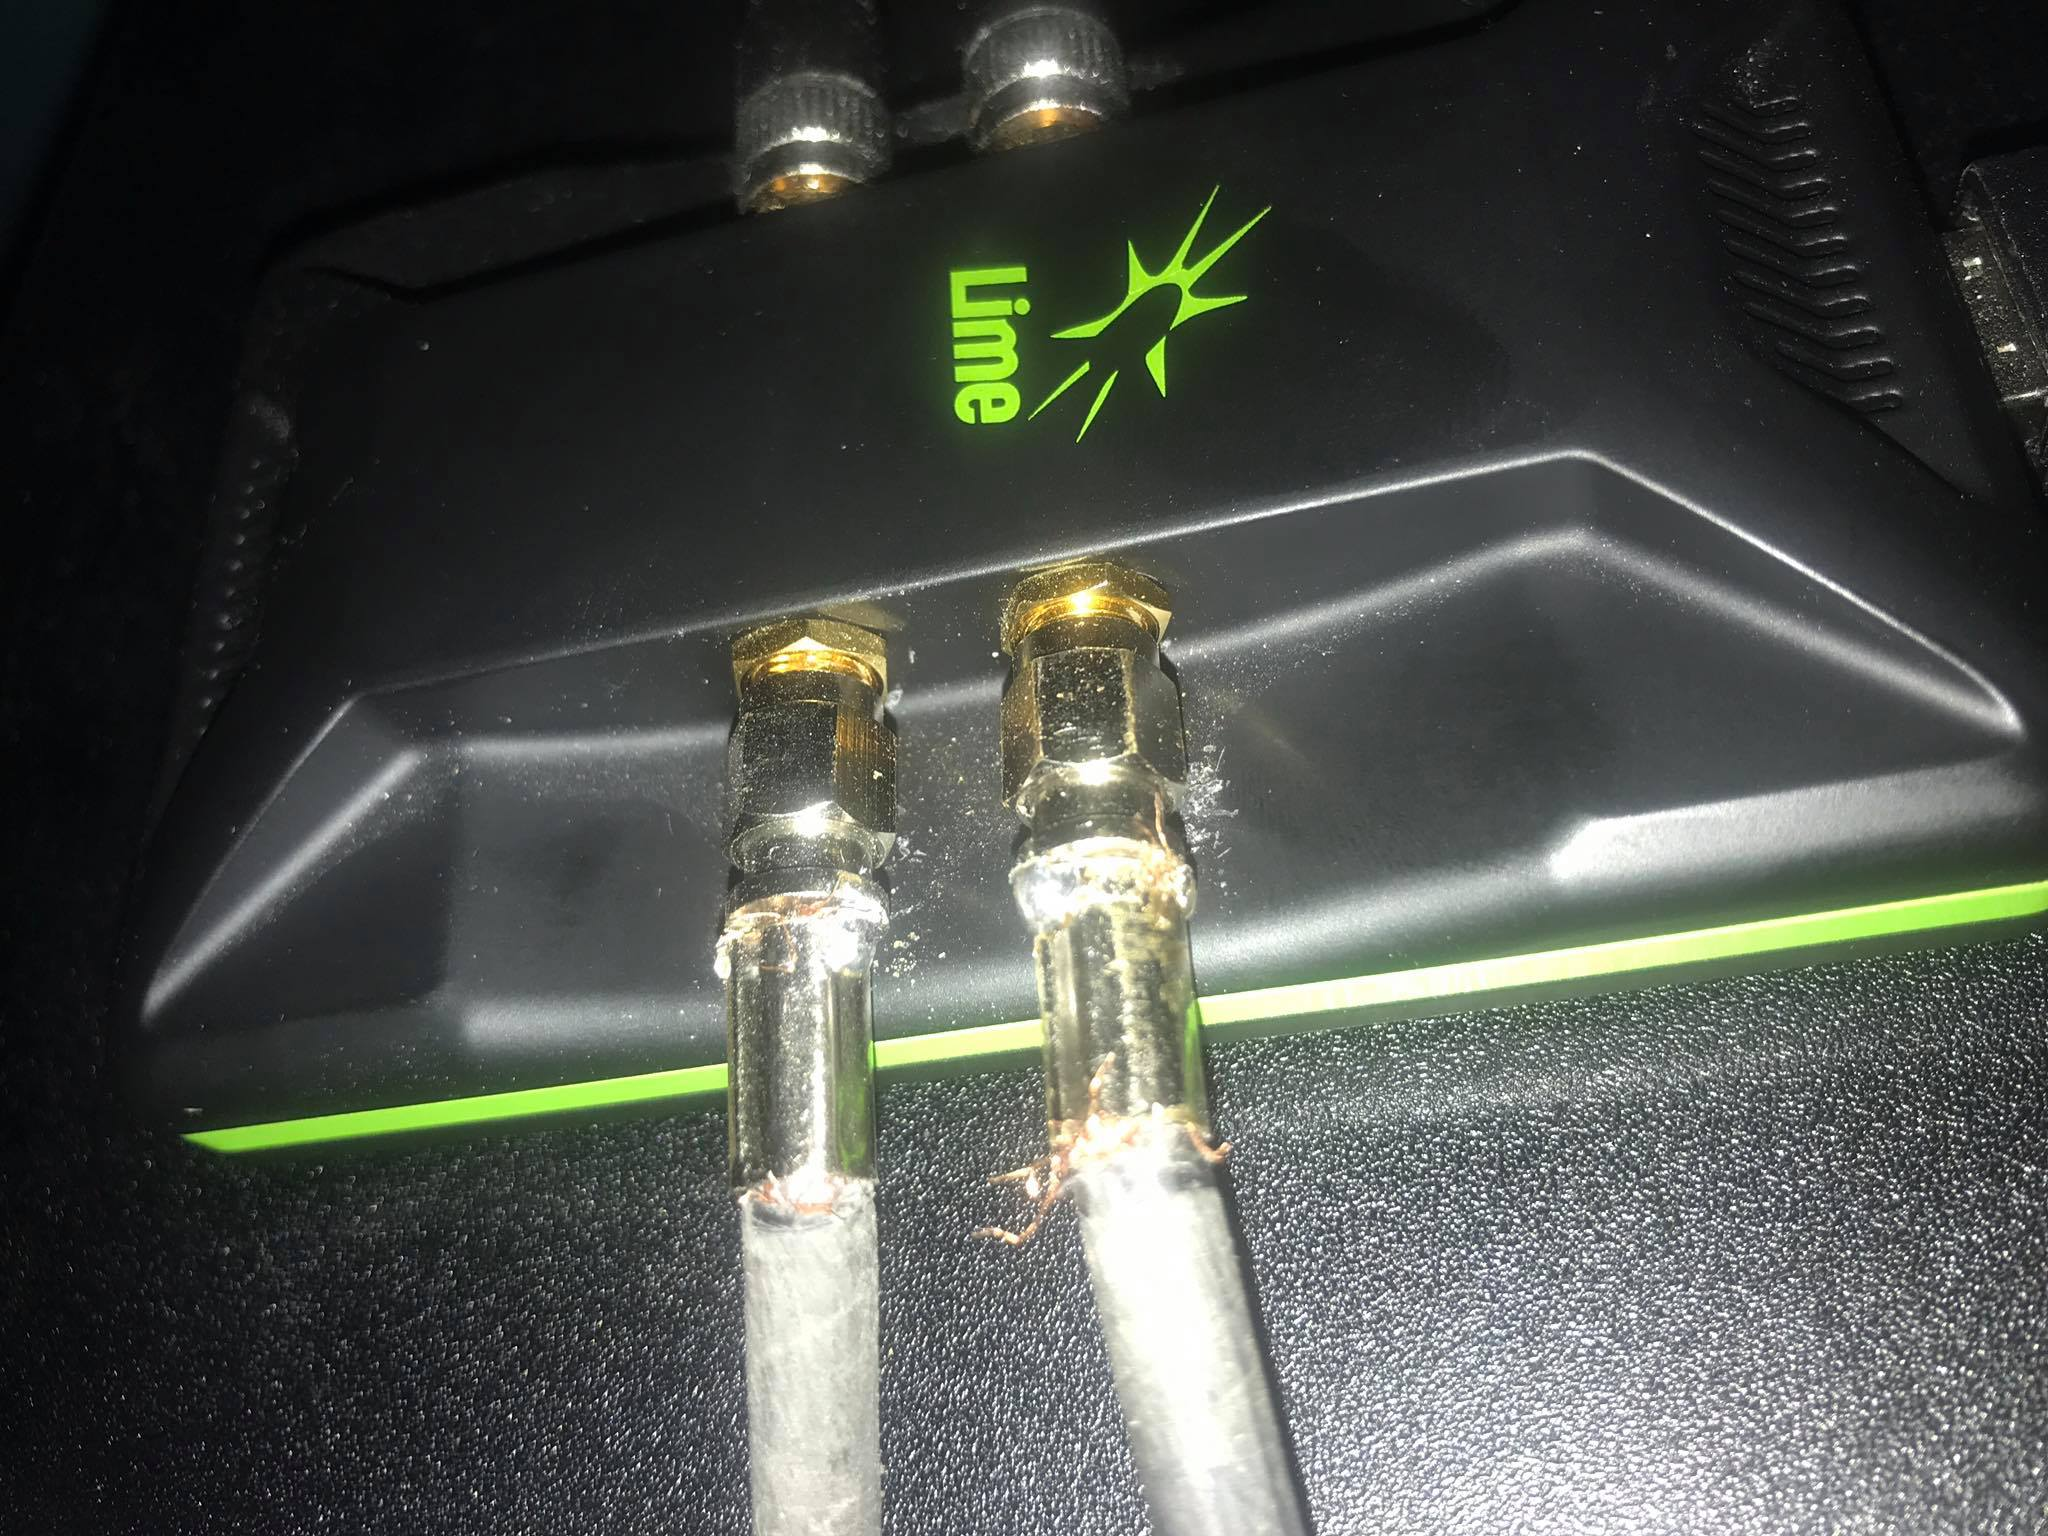
\includegraphics[scale=0.15]{chapters/ch5/assets/limec}
\caption[Entrada LimeSDR]{Entrada LimeSDR}
\label{fig:limec}
\end{figure}

Para o estudo da deteção de alvos utilizando sistemas de deteção passivos, foi utilizado sinais \gls{DVB-T} dos transmissores de Palmela (38°33'23.02"N	8°54'27.56"W) e Cruz de Pau (38°37'3.78"N	9°7'2.31"W), ambos a transmitir nas frequências $598-606 MHz$, e a posição do estudo foi em Brejos de Azeitão (38°32'11.10"N	9°1'21.43"W). Os sinais \gls{DVB-T} são de grande interesse para a deteção com radares passivos como abordado no Capítulo \ref{chap:Chapter1}, visto que entre os disponíveis como iluminadores de oportunidade apresentam uma boa cobertura e uma boa largura de banda, o que se reflete numa boa resolução em alcance. Para uma melhor compreensão do panorama geográfico, a imagem \ref{fig:mapaemi} representa os transmissores a amarelo,  os utilizados a amarelo com um risco preto por baixo e a posição da experiência com um círculo azul.\par 

\begin{figure}[h]
\centering
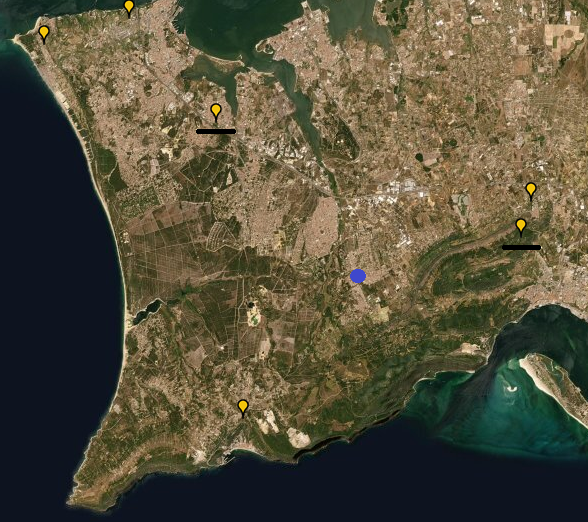
\includegraphics[scale=0.75]{chapters/ch5/assets/mapaemi}
\caption[Mapa de emissores e local da experiência]{Mapa de emissores e local da experiência}
\label{fig:mapaemi}
\end{figure}

Nesta experiência, a antena que recebe o sinal direto estava direcionada para Palmela, recebendo também sinal direto do transmissor da Cruz de Pau devido à pouca diretividade da antena, enquanto a antena que recebe o sinal refletido estava posicionada de modo a apontar noutra direção, como na figura \ref{fig:prat}. Recordando o Capítulo \ref{chap:Chapter3}, chegou-se à conclusão de que as duas antenas ao estarem em sentidos opostos, os lóbulos posteriores iam receber muito sinal indesejado, então mudou-se a geometria da experiência para evitar este problema.

\begin{figure}[h]
\centering
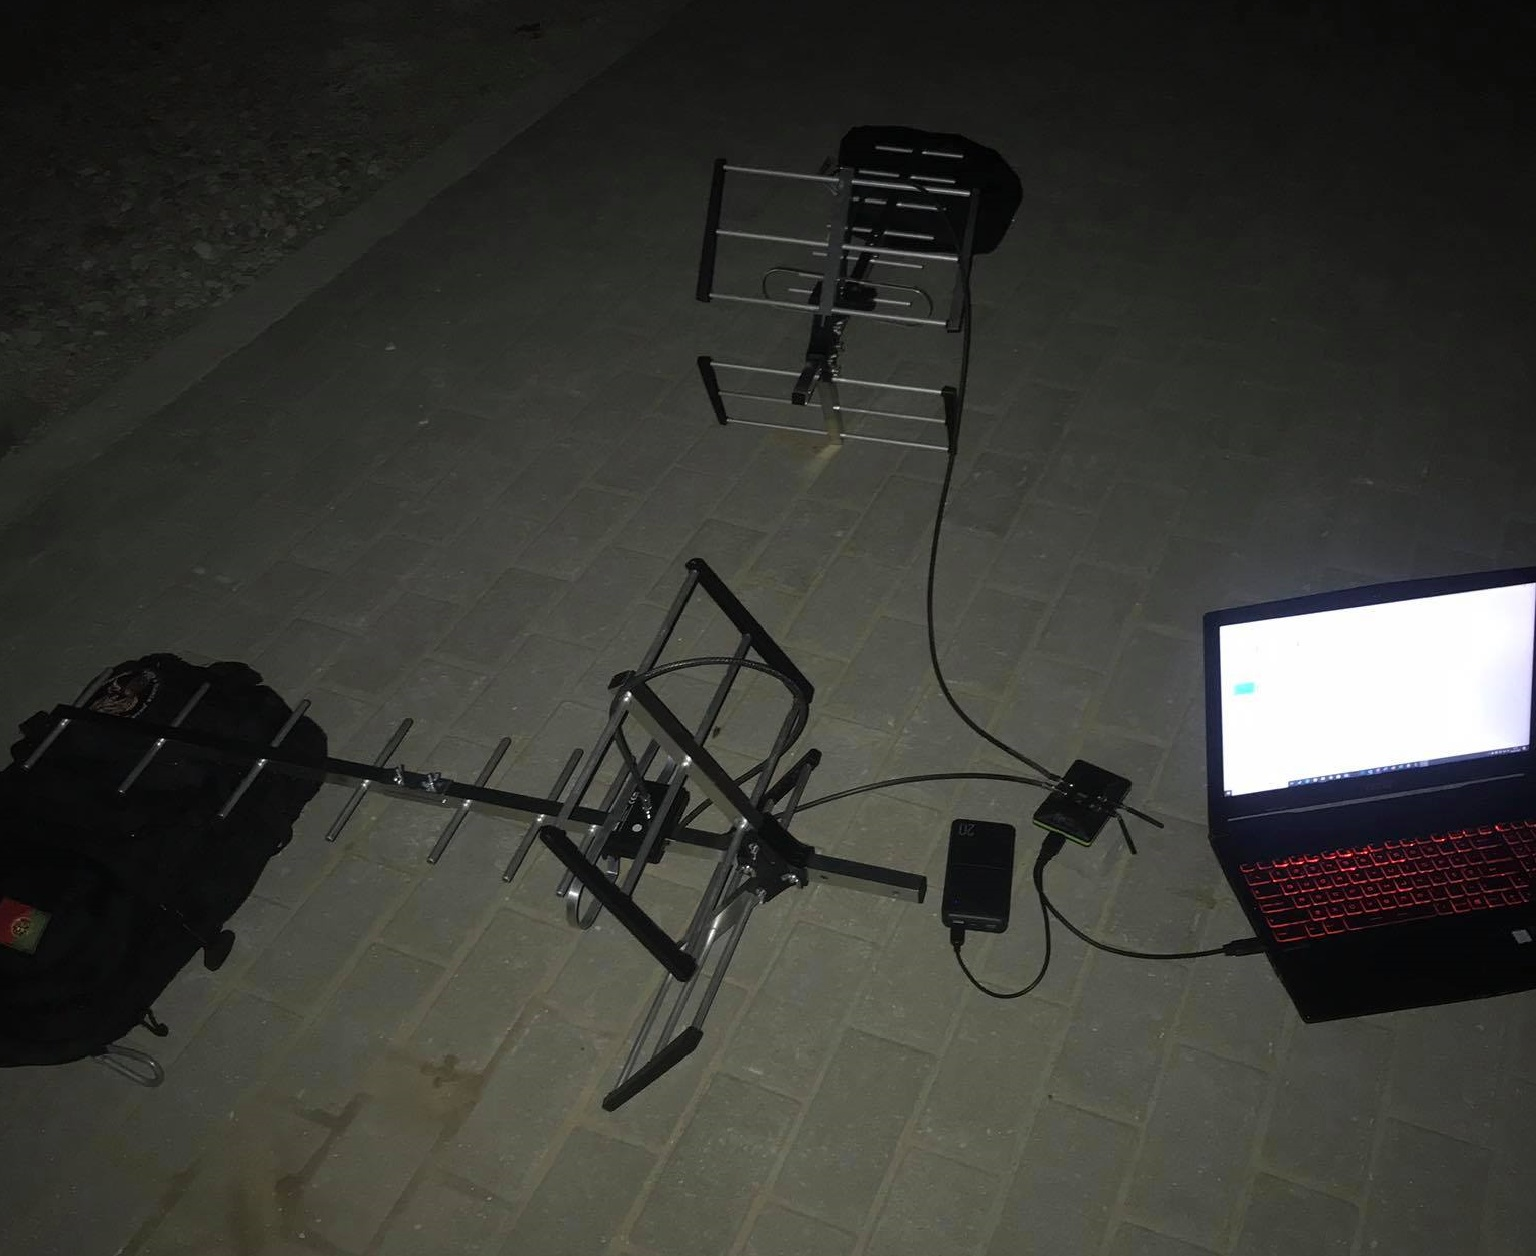
\includegraphics[scale=0.25]{chapters/ch5/assets/prat2}
\caption[Disposição do sistema]{Disposição do sistema no local da experiência}
\label{fig:prat}
\end{figure}

Antes de apresentar os resultados, é necessário compreender a situação em que se está inserido e as limitações do equipamento para se conseguir tirar conclusões coerentes. Com isto, os dois parâmetros a serem considerados inicialmente é a resolução em \textit{Doppler} e em alcance. Da expressão \ref{2.3}, é dada a resolução em alcance para o caso bistático. Visto que o ângulo $\beta$, entre o transmissor e o recetor toma valores perto dos $0^{\circ}$, o termo $cos\left( \dfrac{\beta}{2}\right) = 1$, logo, reduz-se ao caso monostático, e obtém-se o resultado em \ref{5.1}.

\begin{equation} \label{5.1}
\delta_{r}=\dfrac{c}{2B\left( cos\dfrac{\beta}{2}\right)}=\dfrac{3\cdot 10^{8}}{2\times 8\times 10^{6} \left( cos\dfrac{0}{2}\right)}=18.75 m
\end{equation}

Portanto, teoricamente, não é possível distinguir dois alvos com uma distância entre eles menor que $18.75 m$, e logicamente se o alvo estiver em movimento só irá ser detetado a mudança de célula de resolução a cada $18.75 m$.\par 

No caso do desvio de \textit{doppler}, a resolução é dada pela expressão \ref{2.7}, para o caso do recetor estático e alvo em movimento. Desta, para as mesmas condições acima definidas e um tempo de integração de $1 s$, resulta uma resolução em \textit{Doppler} de $2.5 m/s$. No entanto, com um frequência de amostragem utilizada de $17 MHz$ os cálculos são computacionalmente demasiado pesados para o \textit{Matlab} conseguir calcular, para qual a solução ótima seria a aplicação de algoritmos por forma a reduzir este peso, mas a utilizada foi a redução das amostras utilizadas para valores inferiores a $0.1\% $. Isto tem como consequência a diminuição do tempo de integração para $0.1\% \times 1s$ e o agravamento da resolução em \textit{Doppler} para valores extremamente elevados, na ordem das centenas de $m/s$.

\begin{equation} \label{5.2}
\Delta v = \dfrac{\dfrac{3\times 10^{8}}{602\times 10^{6}}}{2\times 1} = 0.25 m/s
\end{equation}



\section{Resultados}
Considerando todas as condições descritas acima para a realização da experiência, os resultados permitiram a deteção do alvo mas com muitas condicionantes, tornando o sistema de baixo custo muito limitado, o que era de esperar.\par  
Todas as amostras foram retiradas com o sistema descrito anteriormente e utilizando o programa no Apêndice \ref{AppendixB}. Inicialmente são introduzidos os parâmetros em variáveis e depois de aberto o \textit{LimeSDR} com o comando \textit{dev = limeSDR()} são inseridos nos dois canais de receção, rx0 e rx1, com a adição do \textit{dev.rx0.antenna = 2} que indica que o \textit{low noise amplifier} a ser utilizados pelo \textit{LimeSDR} é o LNAL, adequado para frequências entre os $0 - 2000 MHz$. Posteriormente os parâmetros são lidos depois de introduzidos para haver registo e verificar se correspondem ao desejado e também é feita a leitura da temperatura do dispositivo visto que este tem tendência a aquecer rapidamente e isto afeta a sua \textit{performance}. De seguida são criadas as matrizes de zeros que vão alojar o sinal recebido, são autorizados os parâmetros nos canais e calibrados os canais de receção para a frequência desejada. Com isto, é iniciado a recolha de dados dos dois canais ao mesmo tempo com o comando \textit{dev.start()} de modo a que as unidades de tempo batam certo nas duas amostras, o que é crucial para que os resultados sejam fidedignos. Durante o tempo de recolha que termina com o comando \textit{dev.stop()}, o sistema vai recolher $Fs*Ts$ amostras no canal 0 e 1 para as variáveis \textit{samples} e \textit{samples1}. Posto isto, é necessário reduzir o numero de amostras para se conseguir fazer a correlação sem que o MATLAB fique sem memória e de seguida, utilizando a função \textit{ambgfun} consegue-se fazer as funções de ambiguidade tanto como a correlação entre os dois sinais recebidos $x$ e $x1$. Finalmente são desenhados os espectro-gramas  dos sinais recebidos tanto como as suas funções de ambiguidade e a correlação.\par 

\begin{figure}[h]
\centering
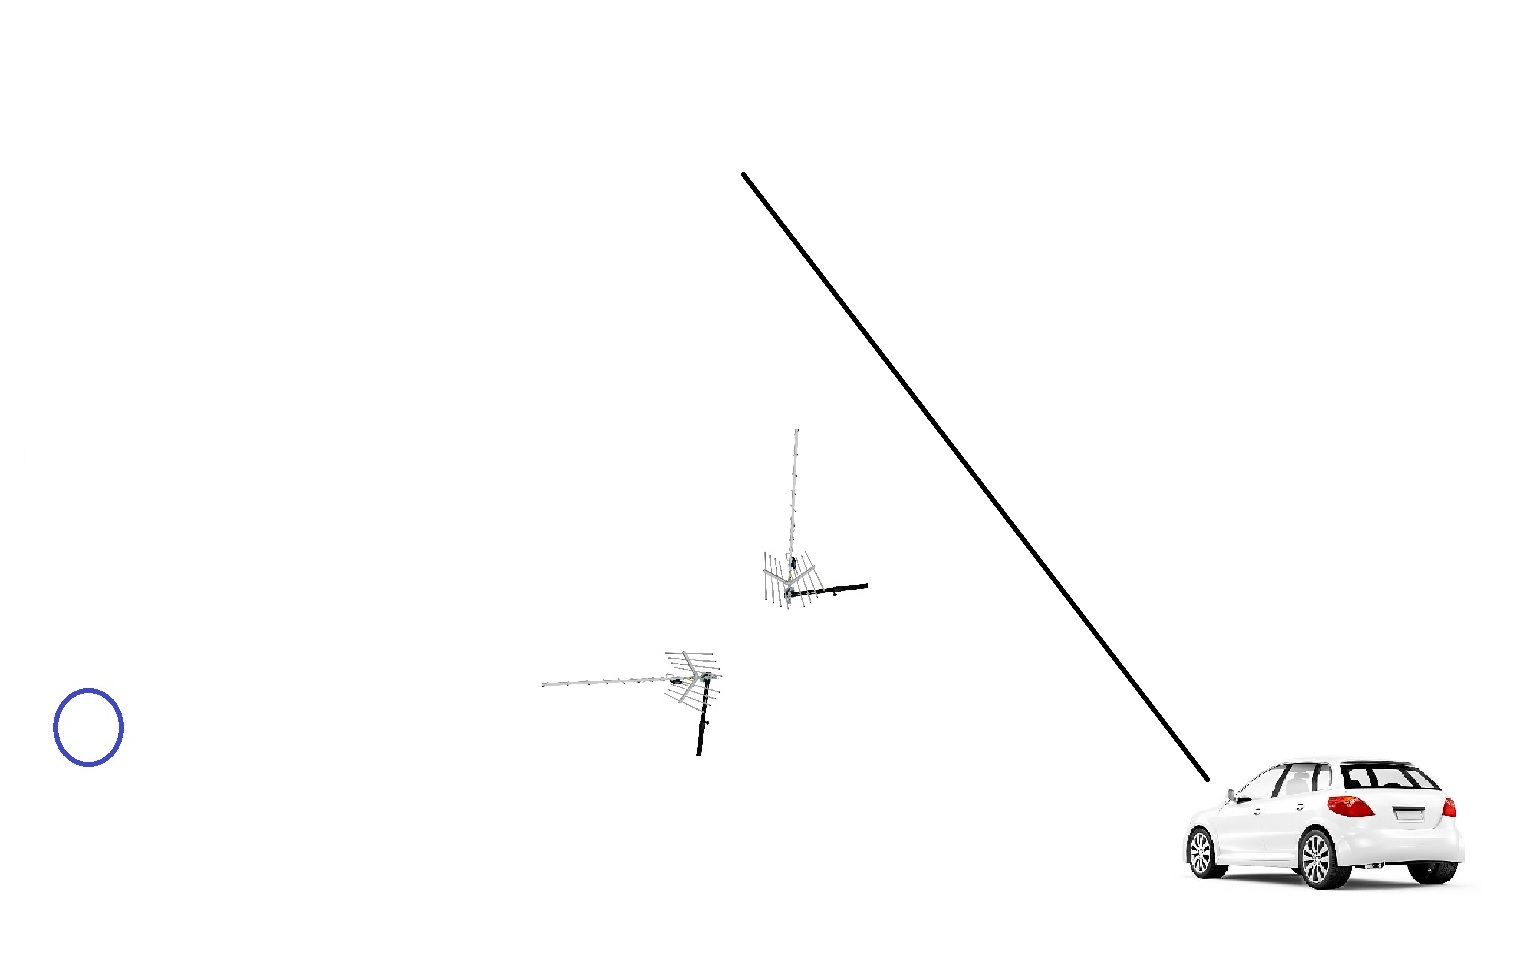
\includegraphics[scale=0.3]{chapters/ch5/assets/geoexp}
\caption[Configuração da experiência]{Configuração da experiência no local}
\label{fig:geoexp}
\end{figure}

A experiência foi dividia em 2 medições:
\begin{itemize}
\item Na primeira, um carro foi metido a $1 5m$ parado com um tempo de integração de $0.2 s$ (figura \ref{fig:15me});
\item No segundo caso, aumentou-se o tempo de integração para $2 s$ e fez-se passar o carro a uma velocidade de aproximadamente $40 km/h$ com uma posição inicial a $15m$ da antena que recebe o sinal refletido e passando a 
$1 m$ desta na sua posição mais próxima, como observável na figura \ref{fig:geoexp}(figura \ref{fig:15mm} e \ref{fig:15mmsum}). 
\end{itemize}

A janela escolhida para o \textit{Delay}, vai do valor $-3\times 10^{-7}$ a $3\times 10^{-7}$, o que segundo a expressão \ref{5.3} onde $t$ representa o \textit{delay} corresponde ao intervalo de $-45 m$ a $45 m$ e cada unidade representa $15 m$. Para a escala de \textit{Doppler}, segundo a expressão \ref{5.4}, para a frequência utilizada, cada $10 m/s = 36 km/h$ representa um desvio em \textit{doppler} de $20 Hz$.

\begin{equation} \label{5.3}
Range = \dfrac{c\times t}{2}
\end{equation}

\begin{equation} \label{5.4}
f_{d} = \dfrac{v}{c}f_{0}
\end{equation}

\begin{figure}[h]
\centering
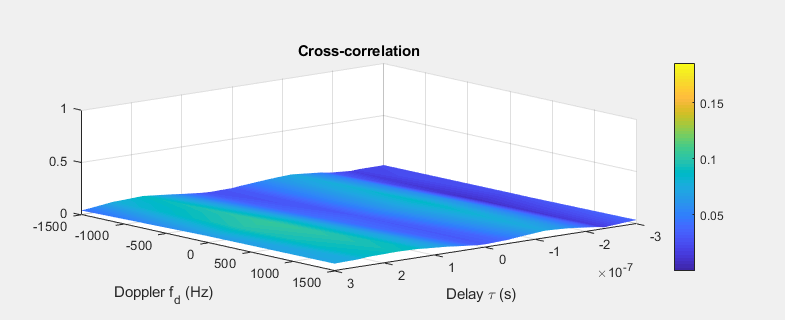
\includegraphics[scale=0.5]{chapters/ch5/assets/15me}
\caption[Caso 1]{Resultado do caso 1}
\label{fig:15me}
\end{figure}

Neste primeiro caso, verificamos a presença do carro na zona do $-1\times 10^{-7}s$ que se extende desde $-0.5\times 10^{-7}s$ a $-2\times 10^{-7}s$ que pode ser justificado com a resolução em alcance calculada com o valor de aproximadamente $19 m$ correspondente a aproximadamente $1.2\times 10^{-7} s$. O facto da frequência estar estendida para valores muito altos tem que ver não só com a resolução em \textit{Doppler} ser muito inadequada, mas maioritariamente pelo desalinhamento na amostragem dos dois canais de receção. Apesar de existir um comando que inicie ao mesmo tempo, o equipamento tem um defeito que desalinha a receção dos dois canais consoante o tempo de integração e a frequência, sendo que quanto maior valor estes tomarem, maior desvio haverá.

\begin{figure}[h]
\centering
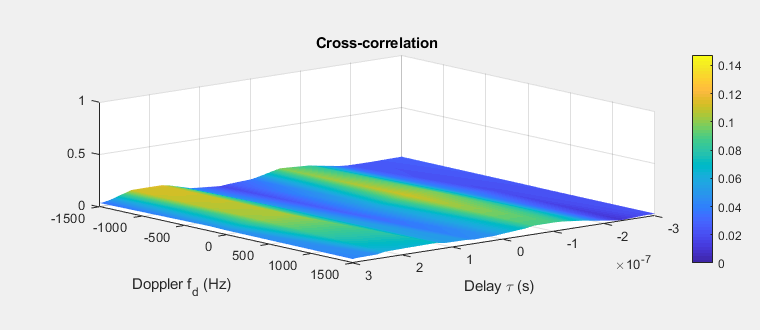
\includegraphics[scale=0.5]{chapters/ch5/assets/15mm}
\caption[Caso 2]{Resultado do caso 2}
\label{fig:15mm}
\end{figure}

Ao analisar o segundo caso, pode-se observar que por aumentar o tempo de integração, aumenta a intensidade da correlação de um alvo em relação às zonas onde não existe correlação.


\begin{figure}[h]
\centering
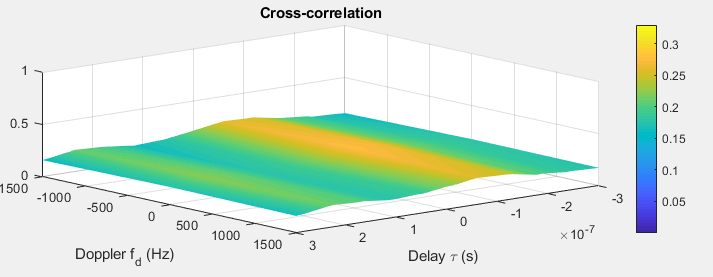
\includegraphics[scale=0.5]{chapters/ch5/assets/15mmsum}
\caption[Caso 2 especial]{Resultado do caso 2 com soma das amostras em diversas partes da matriz}
\label{fig:15mmsum}
\end{figure}

Ainda com os valores do segundo caso, mas somando amostras de diversas partes da matriz, é possível aumentar a intensidade da correlação no alvo se estivermos a utilizar zonas em que o carro se encontrava a refletir mais energia, ou seja, casos em que o carro estivesse mais perto e dentro da zona do diagrama de radiação da antena que tem maior intensidade. Para isto, foram usados os dados gravados do caso 2 e utilizado um programa no Apêndice \ref{AppendixC} que permite escolher as amostras de tempo da matriz que se querem analisar e fazer a correlação em cada uma delas. Uma forma de obter o valor de tempo em que o carro esteve mais perto do sistema é fazer uma correlação apenas em \textit{delay} e ver para que tempo a intensidade é máxima. No caso 2 obteve-se o valor de $0.9 s$ como o tempo em que o carro esteve mais próximo do radar, como se pode observar na figura \ref{fig:4ca}.

\begin{figure}[h]
\centering
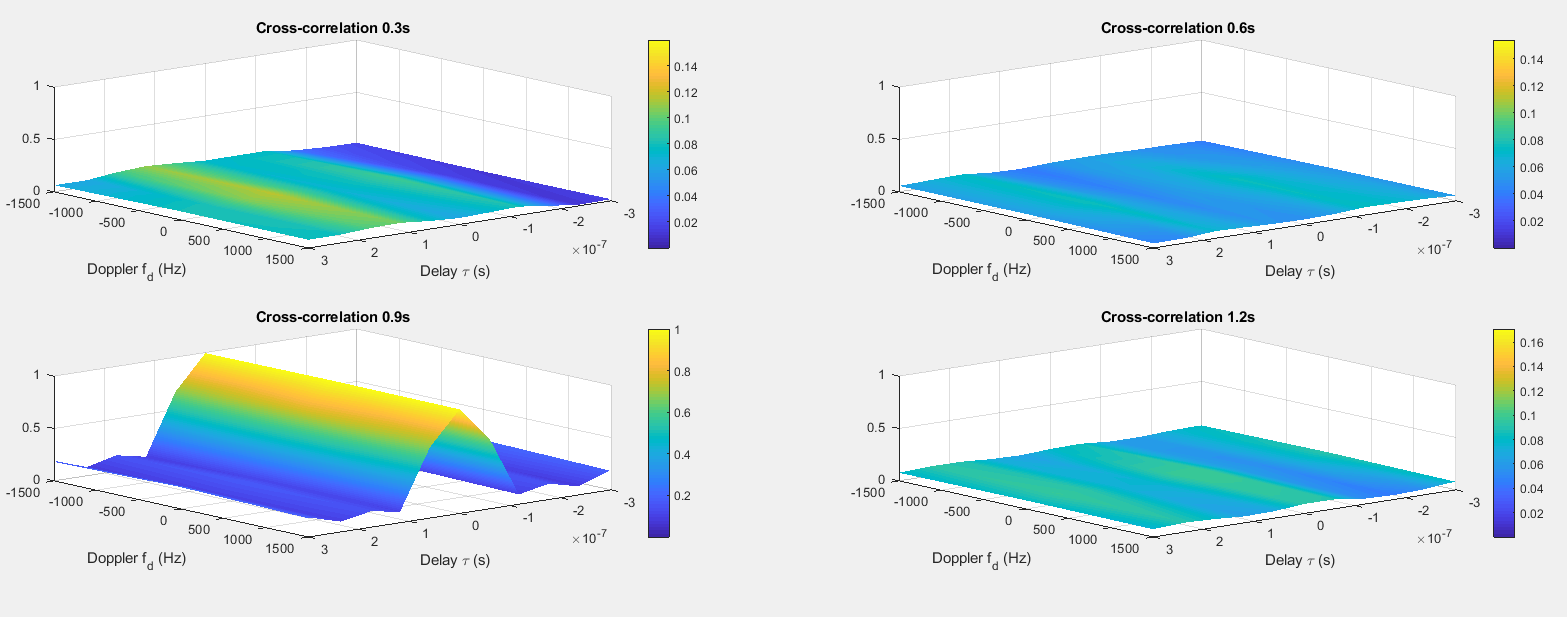
\includegraphics[scale=0.35]{chapters/ch5/assets/4ca}
\caption[Caso 2 dividido em 4 correlações]{Caso 2 dividido em 4 correlações, para $t=0.3s, 0.6s, 0.9s, 1.2s$}
\label{fig:4ca}
\end{figure}



%Conclusão - Obrigatória
% Chapter 6

\chapter{Conclusão} % Main chapter title
\label{chap:Chapter6} % For referencing the chapter elsewhere, use \ref{chap:Chapter6} 

%----------------------------------------------------------------------------------------
\section{Sumário}
O radar passivo é um sistema ótimo para contornar problemas como a deteção através de sistemas de contra-medidas e o elevado preço dos radares convencionais. Também é adequado para a deteção de alvos \textit{stealth} como já falado, devido à sua geometria bistática. No entanto, tudo tem um preço, e o radar passivo não é exceção. Devido ao número elevado de amostras e o processamento do sinal requerido para o tornar viável para a utilização no radar passivo, o sistema fica com um elevado custo computacional e consequentemente existe uma necessidade de processamento digital avançado. Posto isto, deve-se considerar o sistema de radar passivo como um complemento ao sistema de radar ativo, ao invés de uma substituição ao mesmo, visto que cada um colmata os pontos fracos do outro.\par 
Ao aproveitar sinais existentes no espetro eletromagnético, não existe mais poluição do mesmo, mas encontra-se um grande problema, que é o sinal não estar adaptado para a situação em particular tornando o processamento um processo muito mais complexo. Há poucos casos em que o iluminador pode estar adaptado, mas são em situações especificas como a utilização de satélites \gls{SAR} para a formação de imagem.\par 


\section{Discussão e Conclusões}
Seguindo o estudo efetuado durante o trabalho de investigação e do seu complemento com a atividade prática foram retiradas várias conclusões:


\begin{itemize}
\item A dessincronização dos dois canais em tempo é problemática no sentido em que diferença de fase entre o sinal direto e o sinal refletido provoca uma grande distorção em \textit{Doppler}, que é o que se pode verificar em todas as amostras retiradas. Este é um dos principais fatores para existir uma grande dispersão dos alvos em \textit{Doppler}, chegando a ir desde os $-1500 Hz$ aos $1500 Hz$, o que corresponde a uma velocidade de aproximadamente $2700 km/h$. De acordo com \cite{He2010} quanto maior for a velocidade, mais dispersão o sinal tem em \textit{Doppler};


\item A segunda conclusão, como já abordada no Capítulo \ref{chap:Chapter3}, é a pouca diretividade da antena utilizada. O seu diagrama de radiação (\ref{fig:yagi}) apresenta pouca diretividade no lóbulo principal e um lóbulos posterior com muita intensidade. Isto provoca a receção do sinal direto e do refletido na mesma antena o que degrada os resultados tornando-os menos fidedignos;


\item Como terceira conclusão, é importante abordar o tema da reconstrução e equalização do sinal direto, discutido no Capítulo \ref{chap:Chapter4}. A deteção utilizando um radar \gls{PCL} é baseada no cálculo de uma função de ambiguidade cruzada entre o sinal de direto e o refletido no objeto. Idealmente, o sinal recebido na antena de referência a apontar para o transmissor é uma cópia perfeita do sinal transmitido. No entanto, isto não acontece devido ao ruído introduzido e não temos acesso ao sinal direto a partir da localização do recetor, logo, este tem de ser obtido de outra forma. Uma abordagem a este constrangimento é recriar o sinal transmitido através da descodificação do sinal recebido e posterior codificação, obtendo assim uma cópia muito menos ruidosa do sinal transmitido. Ao não utilizar este método, é inserido muito efeito de \textit{multipath} o que prejudica a autenticidade do sinal.


\item Dos resultados do Capítulo \ref{chap:Chapter5} são feitas observações à relação entre o tempo de integração e a intensidade da correlação. De um modo geral, pode-se concluir que ao aumentar o tempo de integração e usando mais amostras, tem-se uma melhor relação sinal-ruído.


\item Ainda do Capítulo \ref{chap:Chapter5} são utilizadas várias amostras e zonas dessas amostras, ou seja, diferentes amostras de tempo do total da amostra. Ao utilizarmos amostras em diferentes marcas temporais somadas, obtemos melhores resultados que utilizando o mesmo número de amostras, mas apenas numa zona da matriz. Isto era de esperar visto que se cobre um tempo de integração maior com o mesmo número de custo computacional.


\item Um problema que afeta imenso a capacidade do radar é ter sido utilizada uma correlação simples. Como abordado no Capítulo \ref{chap:Chapter4}, o custo computacional de fazer uma correlação para milhões de amostras e sabendo que maior tempo de observação resulta em melhor resolução é muito elevado e não é suportável pelas máquinas a que temos acesso diariamente. Isto faz com que seja necessário a implementação de algoritmos que simplifiquem a correlação e contornem o problema do alto custo computacional. Ao não aplicar estes algoritmos os resultados ficam muito degradados, visto que se trabalha com muito menos amostras do que o ideal.


\end{itemize}


Em suma, o sistema de radar \gls{PCL} é muito vantajoso pelas demais razões já identificadas várias vezes e pode-se tornar um sistema muito mais económico, no entanto é necessário um processamento de sinal muito avançado e pesado. A não aplicação de certas técnicas compromete muito a operacionalidade e veracidade dos resultados obtidos pelo radar. Contudo, as conclusões retiradas deste trabalho de investigação permitem guiar futuros projetos e trabalhos de forma a escolher caminhos em que obtenham melhores resultados e permite saber o foco de trabalho para a resolução de determinados problemas.


\section{Cenários Possíveis - MARINHA}
“O projeto DESARMAR é uma iniciativa de investigação para o desenvolvimento de um sistema \gls{SAR} passivo baseado em \gls{SDR} a bordo de um sistema autónomo aéreo para monitorização e proteção do espaço litoral. Este projeto pretende investigar o potencial deste novo tipo de tecnologia e aplica-lo a vigilância e patrulhamento costeiro, fazendo uso de algoritmos de seguimento para identificar eventos de risco e ameaças de origem humana ou natural, permitindo assim a mitigação dos seus impactos (quer de um ponto de vista económico, quer social e ambiental)”. Este trabalho de investigação insere-se neste projeto de forma a contribuir para o estudo nas limitações da deteção utilizando um sistema de radar passivo. O projeto torna-se mais ambicioso com a utilização deste tipo de radares a bordo de um sistema autónomo aéreo e para a formação de imagem, contudo as lições aprendidas com esta dissertação podem direcionar o projeto num caminho mais eficaz.\par
A presente investigação é importante para a Marinha Portuguesa pelo conhecimento deste sistema, que pode ser uma nova realidade com inúmeras aplicações de interesse para a mesma. Um bom exemplo é o projeto \gls{SMARP}, que tem como objetivo projetar e construir uma demonstração de um radar passivo de matriz multi-banda baseado em \gls{SDR} com a finalidade de vigilância da costa.


\section{Propostas para Trabalhos Futuros}
Uma das principais conclusões retiradas desta investigação debruça-se sobre as poucas amostras utilizadas na correlação fazem com que o resultado seja muito degradado relativamente ao que podia ser. A primeira sugestão como complemento deste trabalho é a implementação de algoritmos discutidos ou não no Capítulo \ref{chap:Chapter4} e estudar a melhoria de resultados.\par 
Como segunda sugestão, é interessante realizar um estudo sobre a formação de imagem usando sistemas de radares passivos, o que vai de encontro às necessidades da Marinha e dos seus projetos como o projeto DESARMAR.

%----------------------------------------------------------------------------------------
%	BIBLIOGRAFIA
%----------------------------------------------------------------------------------------

\printbibliography[heading=bibintoc]


%----------------------------------------------------------------------------------------
%	APÊNDICES e ANEXOS
%----------------------------------------------------------------------------------------

% Incluir os apêndices da tese como arquivos separados da pasta (appendices)
% Uncomment as linhas para teres à medida que fores criando apendices.

\appendixfile{appendix1}
\appendixfile{appendix2}
\appendixfile{appendix3}
%\appendixfile{appendix}%


% Incluir os anexos da tese como arquivos separados da pasta (annexes)
% Uncomment as linhas para teres à medida que fores criando anexos

\annexfile{annex1}
%\annexfile{annex2}
%\annexfile{annex3}


%Imprime no documento os anexos e apendices.
\printappendixes
\printannexes

%----------------------------------------------------------------------------------------

\end{document}
